%%%%%%%%%%%%%%%%%%% book.tex %%%%%%%%%%%%%%%%%%%%%%%%%%%%%
%
% sample root file for the chapters of your "monograph"
%
% Use this file as a template for your own input.
%
%%%%%%%%%%%%%%%% Springer-Verlag %%%%%%%%%%%%%%%%%%%%%%%%%%


% RECOMMENDED %%%%%%%%%%%%%%%%%%%%%%%%%%%%%%%%%%%%%%%%%%%%%%%%%%%
\documentclass[graybox,envcountchap,sectrefs, natbib]{svmono}

% choose options for [] as required from the list
% in the Reference Guide

\usepackage{mathptmx}
\usepackage{helvet}
\usepackage{courier}
%
\usepackage[utf8]{inputenc}
%\usepackage[T1]{fontenc}
\usepackage{type1cm}         
%\usepackage{amsmath}
\usepackage{makeidx}         % allows index generation
\usepackage{graphicx}        % standard LaTeX graphics tool
                            % when including figure files
\usepackage{multicol}        % used for the two-column index
\usepackage[bottom]{footmisc}% places footnotes at page bottom
%
%\usepackage{pgfplots}
%\pgfplotsset{compat=1.13}%\pgfplotsset{compat=1.14}
%\pgfkeys{/pgf/number format/.cd,1000 sep={\,}}
%----- Bibliografia ------------
\usepackage{natbib}

\usepackage{chapterbib}
%% ********* Table layout **************
\usepackage{booktabs}
\usepackage{multirow}
\usepackage{tabularx}
\usepackage{tabulary}
\usepackage{tcolorbox}
\usepackage{array}
% see the list of further useful packages
% in the Reference Guide
%% Math Packages %%%%%%%%%%%%%%%%%%%%%%%%%%%%%%%%%%%%%%%%%%%%
\usepackage{amsmath}
\usepackage{textcomp}
%\usepackage{amsthm}
\usepackage{amsfonts}
\usepackage{bm}  %pone en negrita letras griegas
%
\usepackage[nogroupskip, nonumberlist, acronyms]{glossaries}%
\preto\chapter{\glsresetall}
\usepackage{algorithm}
\usepackage{algpseudocode}
\usepackage{matlab-prettifier}
\usepackage{siunitx}
\usepackage{pgfplots}
\pgfplotsset{compat=1.16}
\usepackage{subfig}
\pgfkeys{
	/pgf/number format/.cd,
	set thousands separator={\,},
	min exponent for 1000 sep=4,
}
\makeglossaries
%
\graphicspath{{./figuras/}}
\pdfsuppresswarningpagegroup=1
\newcommand{\xv}{\mathbf{x}}
\newcolumntype{K}[1]{>{\centering\arraybackslash}p{#1}}
\newcommand{\me}{\mathrm{e}}
\newcommand{\md}{\mathrm{d}}


\makeindex             % used for the subject index
                       % please use the style svind.ist with
                       % your makeindex program

%%%%%%%%%%%%%%%%%%%%%%%%%%%%%%%%%%%%%%%%%%%%%%%%%%%%%%%%%%%%%%%%%%%%%
\def\hasbeencalled{0}
\newcommand\matlab{
	\ifnum\hasbeencalled=0
	MATLAB\textregistered{}%
	\global\def\hasbeencalled{1}
	\else
	MATLAB%
	\fi
}
%
\def\hasbeencalledTwo{0}
\newcommand\simulink{
	\ifnum\hasbeencalledTwo=0
	Simulink\textregistered%
	\global\def\hasbeencalledTwo{1}
	\else
	Simulink%
	\fi
}
%%%%%%%%%%%%%%%%%%%%%%%%%%%%%%%%%%%%%%%%%%%%%%%%%%%%%%%%%%%%%%%%%%%%%

\begin{document}
\author{José David Rojas, Orlando Arrieta, Ramon Vilanova}
\title{Industrial PID Controller Tuning}
\subtitle{with a multi-objective framework using MATLAB\textregistered{}}
\maketitle

\frontmatter%%%%%%%%%%%%%%%%%%%%%%%%%%%%%%%%%%%%%%%%%%%%%%%%%%%%%%

%
%%%%%%%%%%%%%%%%%%%%%%% dedic.tex %%%%%%%%%%%%%%%%%%%%%%%%%%%%%%%%%
%
% sample dedication
%
% Use this file as a template for your own input.
%
%%%%%%%%%%%%%%%%%%%%%%%% Springer %%%%%%%%%%%%%%%%%%%%%%%%%%

\begin{dedication}
Use the template \emph{dedic.tex} together with the Springer document class SVMono for monograph-type books or SVMult for contributed volumes to style a quotation or a dedication\index{dedication} at the very beginning of your book in the Springer layout
\end{dedication}





%%%%%%%%%%%%%%%%%%%%%%%foreword.tex%%%%%%%%%%%%%%%%%%%%%%%%%%%%%%%%%
% sample foreword
%
% Use this file as a template for your own input.
%
%%%%%%%%%%%%%%%%%%%%%%%% Springer %%%%%%%%%%%%%%%%%%%%%%%%%%

\foreword

%% Please have the foreword written here
Use the template \textit{foreword.tex} together with the Springer document class SVMono (monograph-type books) or SVMult (edited books) to style your foreword\index{foreword} in the Springer layout. 

The foreword covers introductory remarks preceding the text of a book that are written by a \textit{person other than the author or editor} of the book. If applicable, the foreword precedes the preface which is written by the author or editor of the book.


\vspace{\baselineskip}
\begin{flushright}\noindent
Place, month year\hfill {\it Firstname  Surname}\\
\end{flushright}



%\include{preface}
%%%%%%%%%%%%%%%%%%%%%%acknow.tex%%%%%%%%%%%%%%%%%%%%%%%%%%%%%%%%%%%%%%%%%
% sample acknowledgement chapter
%
% Use this file as a template for your own input.
%
%%%%%%%%%%%%%%%%%%%%%%%% Springer %%%%%%%%%%%%%%%%%%%%%%%%%%

\extrachap{Acknowledgements}

This work wouldn't be possible without the hard work of many students along many years. The authors want to acknowledge the following students which were part of our research lab and made the subject of optimization and PID control part of their academic career:
\begin{itemize}
	\item Macarena Céspedes
	\item Mónica P. Contreras-Leiva
	\item Joaquín Cordero
	\item Carlos Gamboa
	\item Felipe Moya
	\item Gustavo Montoya
	\item Francisco Rivas
	\item Sergio Rodríguez Rojas
	\item Rosario Ruiz Hernández
	\item Felipe Sáenz Cortés
	\item Karen Valverde
	\item Diana Valverde-Mendez
\end{itemize}  

Also, a very special thanks goes to our mentor, professor Víctor M. Alfaro which showed us to love the strange art of industrial PID control.

\tableofcontents

%%%%%%%%%%%%%%%%%%%%%%%acronym.tex%%%%%%%%%%%%%%%%%%%%%%%%%%%%%%%%%%%%%%%%%
% sample list of acronyms
%
% Use this file as a template for your own input.
%
%%%%%%%%%%%%%%%%%%%%%%%% Springer %%%%%%%%%%%%%%%%%%%%%%%%%%

\extrachap{Acronyms}

Use the template \emph{acronym.tex} together with the Springer document class SVMono (monograph-type books) or SVMult (edited books) to style your list(s) of abbreviations or symbols in the Springer layout.

Lists of abbreviations\index{acronyms, list of}, symbols\index{symbols, list of} and the like are easily formatted with the help of the Springer-enhanced \verb|description| environment.

\begin{description}[CABR]
\item[ABC]{Spelled-out abbreviation and definition}
\item[BABI]{Spelled-out abbreviation and definition}
\item[CABR]{Spelled-out abbreviation and definition}
\end{description}
%Definición de símbolos y acrónimos
\newacronym{pid}{PID}{proportional integral derivative}
\newacronym{ws}{WS}{weighted sum}
\newacronym{nbi}{NBI}{normal boundary intersection}
\newacronym{nnc}{NNC}{normalized normal constraint}
\newacronym{ennc}{ENNC}{enhanced normalized normal constraint}
\newacronym{iae}{IAE}{integral of the absolute value of the error}
\newacronym{2dof}{2DoF}{two degrees of freedom}
\newacronym{cerlab}{CERLab}{Control Engineering Research Laboratory}
\newacronym{moo}{MOO}{multiobjective optimization}
\newacronym{moop}{MOOP}{multiobjective optimization problem}
\newacronym{soptd}{ODSOPTD}{overdamped second order plus time delay}
\newacronym{gui}{GUI}{graphical user interface}
%
%------------------------------------------------------------------------
\newglossaryentry{k}{name={\ensuremath{K}},description={Plant gain}}
\newglossaryentry{l}{name={\ensuremath{L}},description={Time delay}}
\newglossaryentry{t}{name={\ensuremath{T}},description={Constant time}}
\newglossaryentry{u}{name={\ensuremath{u(s)}},description={Control signal}}
\newglossaryentry{r}{name={\ensuremath{r(s)}},description={Setpoint}}
\newglossaryentry{y}{name={\ensuremath{y(s)}},description={Feedback signal}}
\newglossaryentry{di}{name={\ensuremath{d_i(s)}},description={Input disturbance signal}}
\newglossaryentry{do}{name={\ensuremath{d_o(s)}},description={Output disturbance signal}}
\newglossaryentry{theta}{name={\ensuremath{\bm{\theta}}},description={Controller parameters vector}}
\newglossaryentry{cont}{name={\ensuremath{C(s,\bm{\theta})}},description={Controller transfer function}}
\newglossaryentry{plan}{name={\ensuremath{P(s)}},description={Plant transfer function}}
\newglossaryentry{beta}{name={\ensuremath{\beta}},description={Weight to the reference signal in the proportional part of the two degrees of freedom controller}}
\newglossaryentry{kp}{name={\ensuremath{K_p}},description={Proportional gain}}
\newglossaryentry{ti}{name={\ensuremath{T_i}},description={Integral time}}
\newglossaryentry{td}{name={\ensuremath{T_d}},description={Derivative time}}
\newglossaryentry{alpha}{name={\ensuremath{\alpha}},description={Filter factor of the derivative part of the controller}}
\newglossaryentry{gamma}{name={\ensuremath{\gamma}},description={Weight to the reference signal in the derivative part of the two degrees of freedom controller}}
\newglossaryentry{contr}{name={\ensuremath{C_r(s,\bm{\theta})}},description={Servo component of the controller}}
\newglossaryentry{conty}{name={\ensuremath{C_y(s,\bm{\theta})}},description={Regulator component of the controller}}
\newglossaryentry{ms}{name={\ensuremath{M_s}},description={Maximum sensitivity}}
%
%-------------------------
%\printglossaries[title=Symbols and Abbreviations]
%\extrachap{Acronyms}
\printglossary[type=\acronymtype, title= Abbreviations]
\mbox{}
\printglossary[title= Symbols]


\mainmatter%%%%%%%%%%%%%%%%%%%%%%%%%%%%%%%%%%%%%%%%%%%%%%%%%%%%%%%
%
\chapter{Introduction}
%\begin{refsection}
\label{sec:Antecedentes}
The design of control systems always has to consider multiple and possibly conflicting design objectives. Under this perspective, the task of the engineer in charge of the control system, becomes to find the optimal point of compromise within this set of distinct objectives \citep{Garpinger2012}.

The most used control algorithm in industry is the \gls{pid}. This type of algorithm is used in a wide variety of applications, due to its limited number of parameters, its ease of implementation and its robustness \citep{astromhagglund2006} and represents an area of active study since the first tuning methodology was proposed in the 1940s \citep{Ziegler1942}.

It is common practice that the problem of tuning the parameters of industrial controllers is posed as an optimization problem. When all the objectives need to be taken into account at the same time, this problem becomes a multivariable, multiobjective optimization problem. In the particular case of industrial \gls{pid} controllers, this problem is also non-linear and (possibly) non convex, therefore, the problem at hand is not trivial.

Regardless of the methodology to be used, it is generally computationally expensive to solve a multiobjective optimization problem, which can lead to a scenario of multiple equally optimal solutions, so that in addition to solving the optimization problem, the control engineer, ends up with the extra responsibility of entering into a posteriori decision phase  to finally choose the best set of parameters for its specific application.

In this sense, \gls{moo} tuning of \gls{pid} controllers remains as an open research subject, even though it has bee studied for several decades. For example, in \citet{Seaman1994} a type of \gls{moo} is used to tune \gls{pid} controllers in a plastic injection molding process. In \citet{Abbas1995}, an algorithm based on several optimizations is proposed to find the optimal parameters of a \gls{pid} controller; this algorithm took into account several variables such as stationary error, rise time, overrun, settling time and maximum controller output within the feedback loop. More recently, bio-inspired techniques such as neural networks, fuzzy logic or genetic algorithms have been used to solve the optimization problem \citet{Reynoso-Meza2012b}. In \citet{Bagis2011}, A Tabu search algorithm is used to tune \gls{pid} controllers in real time, based in a set of closed loop specifications and a cost function. In \citet{Chiha2012} the \gls{moop} for \gls{pid} controllers is solved using the ant colony approach, this methodology tries to simulate the behavior of real ants when they are looking of the shortest path to a given objective.

Besides bio-inspired methods for \gls{moop}, there are several methdologies that transform the \gls{moop} into a single function optimization problem, by rewriting the problem with extra constrains. The simplest method is the \gls{ws} \citep{Marler2004}. With the \gls{ws} method, the multiobjective cost function is transformed into a one dimensional function using a weighted sum that gives a greater relative weight to a function in comparison to the others. For each set of weight values a different optimal solution is found for the same problem. The set of all solutions is part of the Pareto front \citep{Marler2004}. The Pareto front corresponds to all equally optimal solutions for a \gls{moop}. The problem with the \gls{ws} method is that, although the results obtained are from the Pareto front, it is not possible to satisfactorily construct the entire front \citep{Das1997,Messac2000,Marler2010}.

In order to obtain the Pareto front correctly, other methodologies have emerged that surpass the \gls{ws}. The \gls{nbi} method consist in rewriting the optimization problem so that the feasible area is shortened by an equality constraint that depends on an extra parameter \citep{Das1998}. The solution of this new problem will terminate at the Pareto border and by varying this extra parameter, it is possible to find the Pareto front so that each found point is equally spaced at the front. This feature is very useful since it gives an overall idea of the shape of the front. \gls{nbi} has been applied to the tuning of controllers in \citet{Gambier2009} where the controller is selected taking into account different performance indexes like the integral of the squared error (ISE), the integral time-weighted squared error (ITSE) and the integral of the squared time-weighted squared error (ISTSE). Other methodology similar to \gls{nbi} is the \gls{nnc} \citep{Messac2003}, which converts the \gls{moop} in a single function optimization with an extra inequality constraint.

It should be noted that these methodologies have also been used in other areas apart from the control of industrial processes. A few examples of the areas in which it has been applied are: calculation of optimal power flow in power systems \citep{Roman2006}  and distributed generation planning \citep{Zangeneh2007},  for the control of biochemical processes \citep{Logist2009}, circuit analysis \citep{Stehr2003}, development of optimal supply strategies for the participants of oligopolistic energy markets \citep{Vahidinasab2010}.

The objective of this book is to present the methodology to tune \gls{pid} controllers as a \gls{moo} problem. Along the book, several industrial examples are taken into account to exemplify the concepts and gain insight into the application. With some sections of the book, a companion software written on \matlab is included. The idea with the software is to be as open as possible, the reader will be able not only to have access to the code, but also to the data base that was obtained while solving the \gls{moop}.

On Chapter~\ref{chap:IndustrialPID} the fundamental concepts of process control are presented to set the basic foundations of this book. An Isothermal Continuously Stirred Tank Reactor is used as example to explain the methodology that is employed within the control field. On Chapter~\ref{chap:PIDControllerConsideration} the metrics used for performance and robustness are presented for the case of \gls{pid} control along with the tradeoffs that arises in a controlled system are considered, for example the well known relationship between servo and regulation responses, or between performance and robustness.

Chapter~\ref{chap:PIDControllerDesign} presents the foundation of \gls{pid} tuning, first the analytical tuning methods are presented in order to have the mos fundamental mathematical description of a tuning rule. Then, the tuning based on the minimization of a performance criteria is considered. This subject is important for this particular book because the methodology that is presented is based on the minimization of multiple cost functions at the same time.

From Chapter~\ref{chap:Multi-objective} until the end of the book, the multiobjetive case is considered. Particularly in this chapter, the basic formulation of the optimization problem is presented with the introduction of the Pareto front concept. The methodology chosen to solve the multiobjective optimization problem is to transform the multi-criteria situation into a single scalar cost function. A wastewater treatment plant model is used as example on how the Pareto can be applied to industrial processes.

The \gls{moo} techniques are tested and applied to different scenarios on Chapter~\ref{chap:ApplicationExamplesNoGUI}. Different scalarization techniques are tested and the methodology is applied to a LiTaO$_3$ Thin Film Deposition Process. On Chapter~\ref{chap:PIDMOOP}, the \gls{pid} tuning problem stated in Chapter~\ref{chap:PIDControllerDesign} is solved using the ENNC methodology presented in Chapter~\ref{chap:Multi-objective}. First the problem is solved using a \matlab script that can be found in the appendix of this chapter and also downloaded as a companion software. The result of this script is a set of files that defines 2200 Pareto fronts with the optimal solutions of the problem of finding the tuning of \gls{2dof} \gls{pid} controller for \gls{soptd} plant families. Then two possible approaches are presented to use this results: first an attempt to find a tuning rule based on this data is presented. This approach was found to be very difficult to apply given the complexity of the data. Then the data was used as a data base and a GUI was created to serve as the bridge between the user and the results. This GUI was encapsulated as a MATLAB app and included as the companion software for this book.

Finally, on Chapter~\ref{chap:ApplicationExamples} different examples are provided to exemplify the application of the tool presented in this book. The software is used to analyze the temperature control in a Continuously Stirred Tank Heater and the concentration of the product in an isothermal Continuosly Stirred Tank Reactor.

\bibliographystyle{spbasic}
\bibliography{ReferenciasMulti}
\chapter{Industrial PID Control}
\label{chap:IndustrialPID}
\abstract*{abstract (10--15 lines long)}

\abstract{abstract (10--15 lines long)}

\section{Control System Design Scenario}
\label{sec:1}

Control systems are used to maintain process conditions at their desired values by manipulating certain process variables to adjust the variables of interest. A common example of a control system from everyday life is the cruise control on an automobile. The purpose of a cruise control is to maintain the speed of the vehicle (the controlled variable) at the desired value (the set point) despite variations in terrain, hills, etc. (disturbances) by adjusting the throttle, or the fuel flow to the engine (the manipulated variable). Another example is the home thermostat. This control system is designed to maintain the temperature in the home at a comfortable value by manipulating the fuel flow or electrical input to the furnace. The furnace control system must deal with a variety of disturbances to maintain temperature in the house, such as heat losses, doors being opened and hope- fully closed, and leaky inefficient windows. The furnace must also be able to respond to a request to raise the desired temperature if necessary. For example, we might desire to raise the temperature by 5?? degrees and we would like the system to respond smoothly and efficiently. From these examples, we can deduce that there are several common attributes of control systems:
\begin{itemize}
\item The ability to maintain the process variable at its desired value in spite of disturbances that might be experienced (this is termed disturbance rejection)
\item The ability to move the process variable from one setting to a new desired setting (this is termed set point tracking)
\end{itemize}

A natural way to adjust or correct the behaviour over time of a dynamic system output, the controlled variable, is by using an actuating input computed on the basis of the comparison of the actual output with its desired value: the feedback error. This is, by means of closed-loop control. To compute the control action information about the feedback error evolution is required. Normally its current value, its past evolution, and a prediction of its future behaviour are used. The way we use this information to deliver the control action constitutes the control algorithm. Conceptually we can view the control systems in the general manner shown in figure (\ref{Ch2fig:FeedbackControlSystem}).

\begin{figure}[tb]
\centering
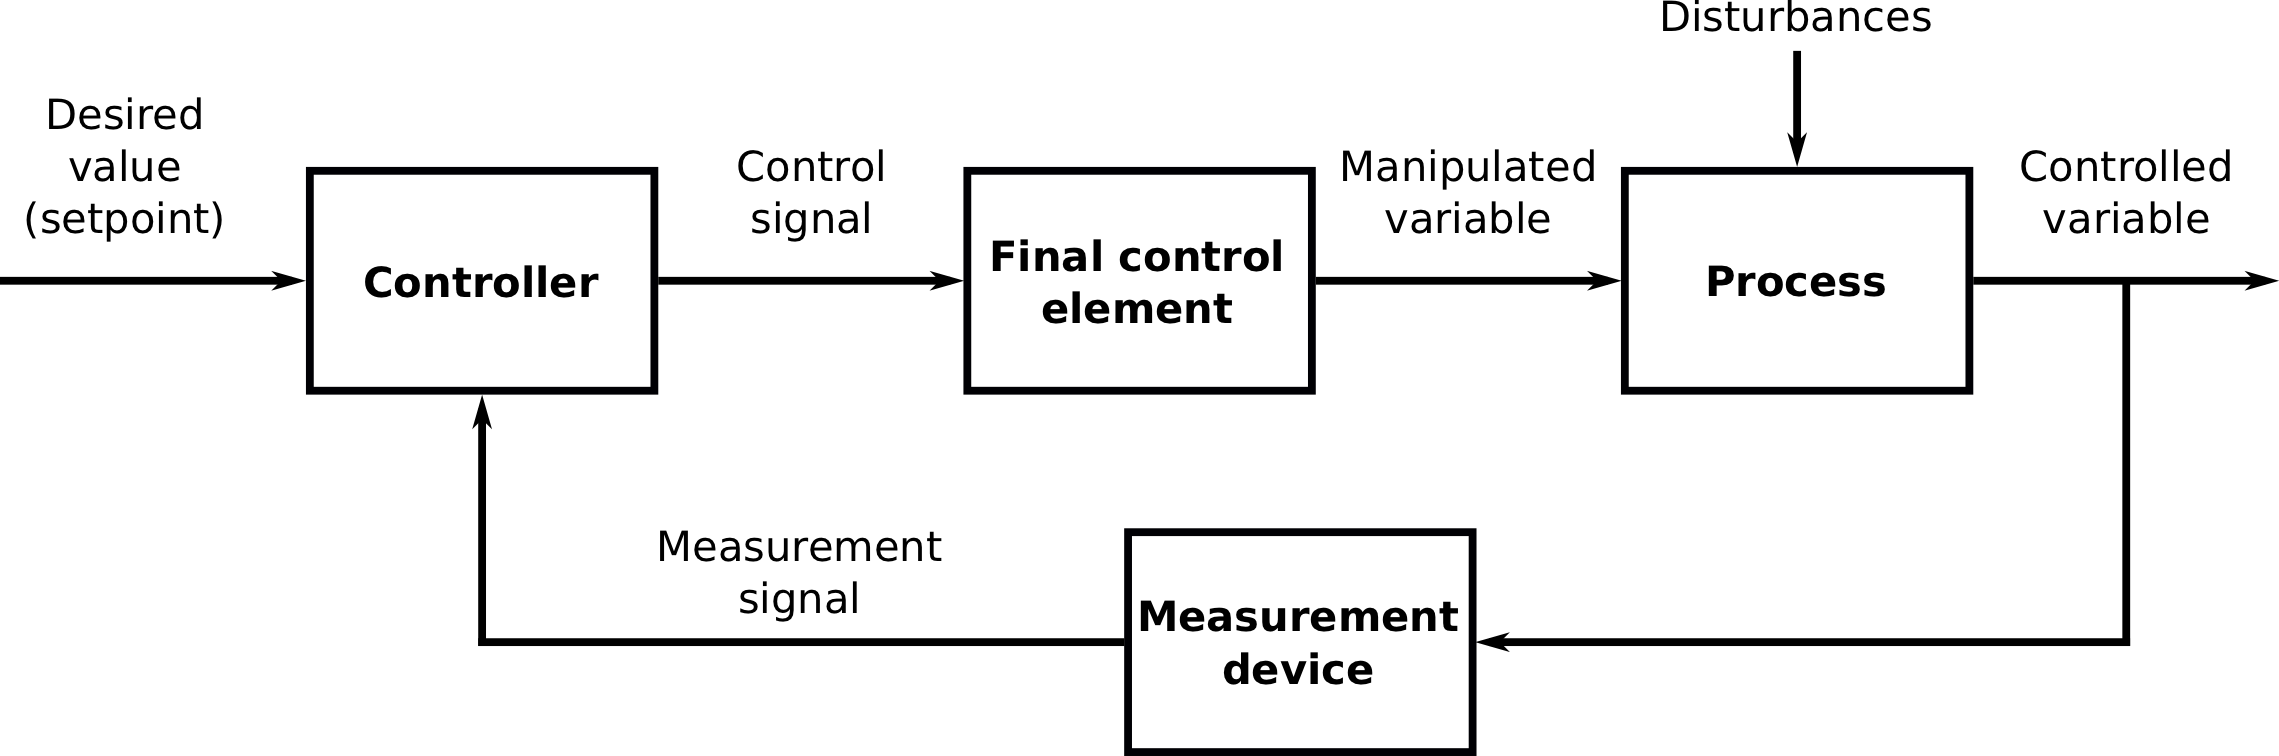
\includegraphics[width=0.9\linewidth]{../figuras/Ch2FeedbackControlSystem}
\caption{Feedback Control System} \label{Ch2fig:FeedbackControlSystem}
\end{figure}

As a detailed  practical example, consider the isothermal Continuous Stirred Tank Reactor (CSTR), as the one in figure (\ref{Ch2fig:CSTR}), where the isothermal series/ parallel Van de Vusse reaction \cite{arrietaETFA2008}, \cite{VandeVusse2} ISA-d takes place. The reaction can be described by the following scheme

\begin{align}
    A \overset{k_1}{\longrightarrow} B \overset{k_2}{\longrightarrow}C\\
    2 A \overset{k_3}{\longrightarrow} D \nonumber
\end{align}

\begin{figure}[tb]
\centering
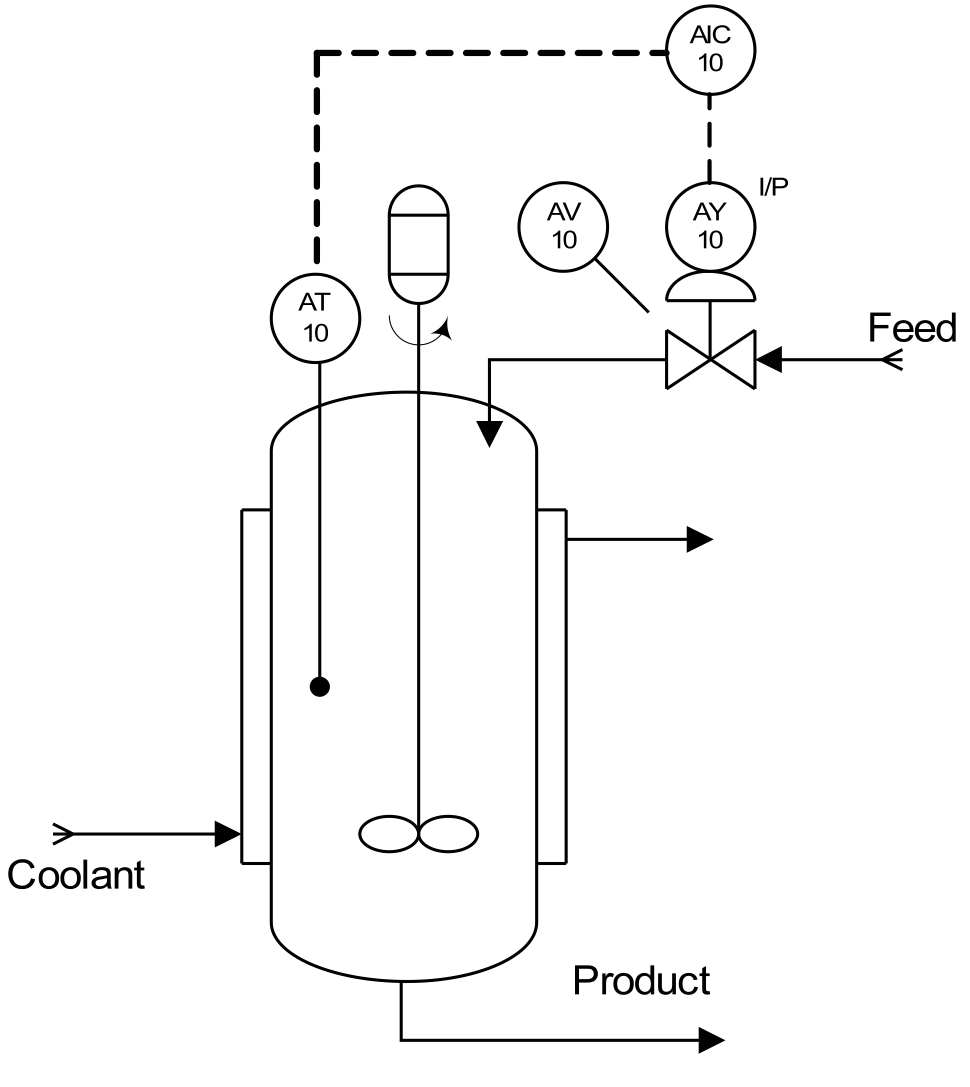
\includegraphics[width=0.5\linewidth]{../figuras/Ch2Reactor}
\caption{Isothermal Continuous Stirred Tank Reactor (CSTR)} 
\label{Ch2fig:CSTR}
\end{figure}

Doing a mass balance, the system can be described by the following model

\begin{align}
    \frac{dC_A(t)}{dt} & = \frac{F_r(t)}{V} \left[C_{Ai}-C_A(t)\right] - k_1 C_A(t) - k_3 C^2_A(t) \nonumber \\
    \frac{dC_B(t)}{dt} & = -\frac{F_r(t)}{V} C_B(t)+ k_1 C_A(t) - k_2 C_B(t)
    \label{Ch2eq:system3}
\end{align}

\noindent where $F_r$ is the feed flow rate of product $A$, $V$ is the reactor volume which is kept constant during the operation, $C_A$ and $C_B$ are the reactant concentrations in the reactor, and $k_i$ ($i=1,2,3$) are the reaction rate constants for the three reactions.\\

\textcolor{red}{\bf EXPLICAR VARIABLES, CONTROLADA, PERTURBACIONES, MANIPULADA, ETC}

In figure (\ref{Ch2fig:CSTRFigureOpenLoop}) we can observe how the reactor output concentration reacts to changes in each one of its two inputs: The inlet flow rate, $F_r$ and concentration $C_A$. Whereas the first one can be manipulated the second one is considered now know as supplied externally. Therefore, $F_r$ is considered as the manipulated variable and will be the one used to operate and control the reactor. On the other hand, changes in $C_A$ will be seen as disturbances and the controller should be able to counteract such changes and prevent them to generate changes in the output concentration $C_B$. 

\begin{figure}[tb]
\centering
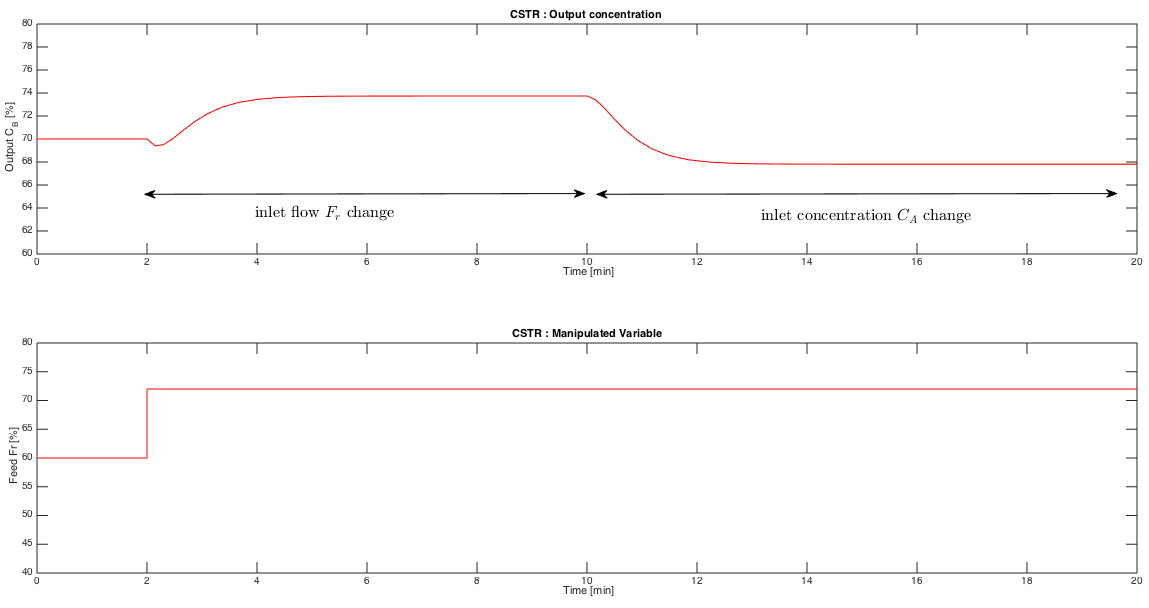
\includegraphics[width=1\linewidth]{../figuras/Ch2FigureOpenLoop}
\caption{CSTR Open loop Output to change sin inlet flow and concentration} 
\label{Ch2fig:CSTRFigureOpenLoop}
\end{figure}


The feedback control structure has been used for a long time, but if we constraint ourselves to the industrial process control area, the proportional (present) integral (past) derivative (future) (PID) control algorithm age starts in the 40's  with the PID controller and this will be the concern of this text.  A control algorithm has a number of control parameters, which must be \emph{tuned} (adjusted) to have acceptable performance. Often the tuning is done on a simulation model before implementing the control strategy on the actual process. In this text ww will concentrate on the determination of the controller tuning, in fact, PID tuning, by means of optimisation methods. Specifically, optimisation methods that deal with multiple objectives at the same time. However, prior to this task, we should define the control scenario where the design will take place.\\

Consider the general two-degree-of-freedom closed-loop control system depicted in figure~\ref{Ch2fig:DoFControlSystem} where $P(s)$ and $\{C_r(s), C_y(s)\}$ are the controlled process model and the controller transfer functions, respectively.  In this system, $r(s)$ is the set-point, $u(s)$ the controller output signal, $d(s)$ the disturbance, $y(s)$ the process controlled variable, and $n(s)$ the measurement noise. It is assumed that the disturbance enter at the process input (load-disturbance).

\begin{figure}[tb]
\centering
	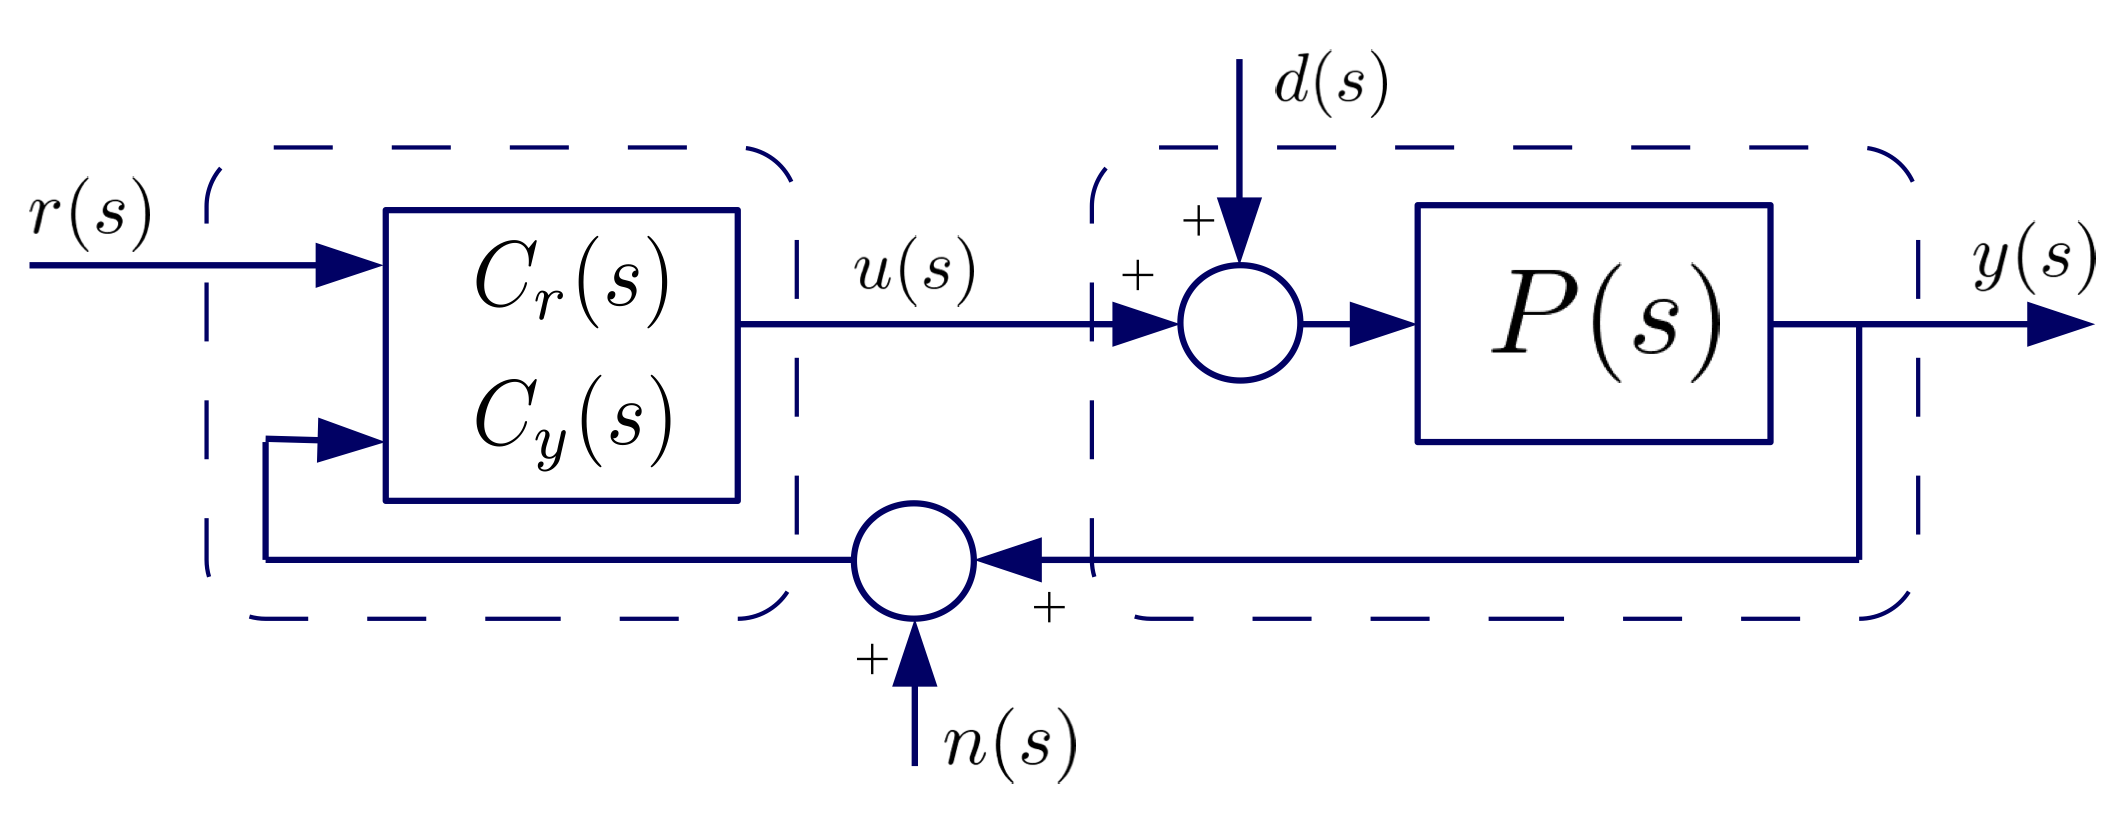
\includegraphics[width=0.5\linewidth]{../figuras/Ch2DoFControlSystem} 
\caption{Two-Degree-of-freedom closed-loop control system.} 
\label{Ch2fig:DoFControlSystem}
\end{figure}


The closed-loop control system output $y(s)$ as a function of its inputs $r(s)$, $d(s)$, and $n(s)$ is

\begin{equation}
	y(s) = M_{yr}(s) r(s) + M_{yd}(s) d(s) + M_{yn}(s) n(s), \label{Ch2eq:yt}
\end{equation}

\noindent where
\begin{equation}
	M_{yr}(s) \doteq \frac{C_r(s)P(s)}{1+C_y(s)P(s)}, \label{Ch2eq:myr}
\end{equation}

\noindent is the servo-control closed-loop transfer function, 
\begin{equation}
	M_{yd}(s) \doteq \frac{P(s)}{1+C_y(s)P(s)}, \label{Ch2eq:myd}
\end{equation}

\noindent the regulatory control closed-loop transfer function, and
\begin{equation}
	M_{yn}(s) \doteq \frac{-C_y(s)P(s)}{1+C_y(s)P(s)}, \label{Ch2eq:myn}
\end{equation}

\noindent the measurement noise sensitivity function.\\

The regulatory control main objective is \emph{load-disturbance rejection}; this is, to return the controlled variable to its set-point in the event a disturbance enters to the control system.  For the servo-control, it is intended to \emph{follow a changing set-point}; this its, to bring the controlled variable to its new desired value. Controller tuning for above operations must take also into account to not amplified the measurement noise, if any.  In figure (\ref{Ch2fig:CSTRFigureClosedLoop}) we can see the CSRT example presented above, where a controller, is accomplishing the task of, first, tracking a set-point step change of, followed by a disturbance attenuation  of two changes. One  in the concentration, $C_{Ai}$, of $A$ in the feed flow and finally a change in the supplied flow rate.

\begin{figure}[tb]
\centering
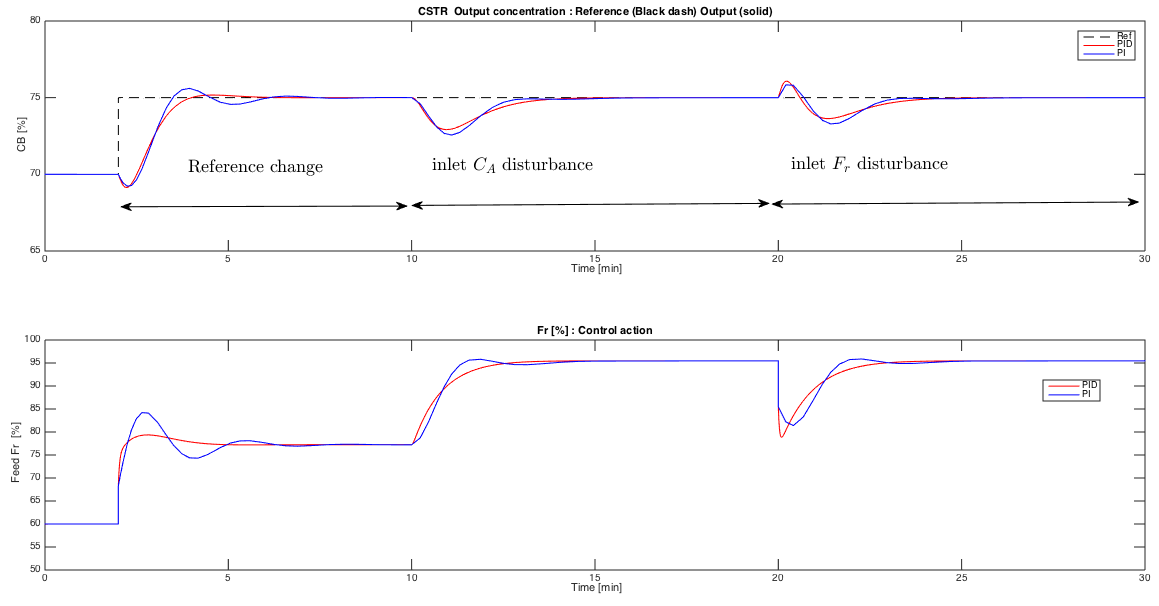
\includegraphics[width=1\linewidth]{../figuras/Ch2FigureClosedLoop}
\caption{CSTR Open loop Output to change sin inlet flow and concentration} 
\label{Ch2fig:CSTRFigureClosedLoop}
\end{figure}


\section{Industrial Process Characteristics}
\label{sec:2}

Before a controller for a process is specified, the process to be controlled should be characterised, at least in some broad sense. There are many different types of processes that are controlled automatically. Examples range from fluid levels in tanks to read-write heads of computer disk storage devices. The control inputs to a process are supplied through one or more actuators. For example a motor driven valve can be an actuator for fluid flowing into a tank. Process outputs that are being controlled (e.g., the fluid level in a tank) are measured using appropriate sensors. The basic control of one output variable by the use of one control input variable is called single-input single-output (SISO) control. For more complex systems, multi-input multi-output (MIMO) control may be required. PID control was developed initially as a SISO control strategy, but it has been extended in various ways to MIMO control \cite{wang2008}. Event these extensions, it is common practice in the process industry to rely on PID control at single loop level control problems, whereas multivariable control solutions, such as model predictive control are the ones applied for multivariable and supervisory control [REF].\\

In the great majority of process loops, applying a step to the control variable causes the controlled variable to reach a steady state and does not provoke an instantaneous variation of it. This means that the process model seen by the regulator can be described by an asymptotically stable, strictly proper transfer function. FOPTD dynamics are probably the most usual models used in the process industry for modelling self-regulating behaviours. For example when modelling dynamics that involve balances of temperature, matter, and energy in general. Also in a reactor where a reaction takes place, the components balance generates a dynamics that can be usually modelled as a FOPTD. When different reactors are connected in series, higher order systems arise that can be described by SOPTD models. \\

In a few loops, a control step causes the controlled variable to asymptotically assume a ramp-like behaviour. This case is commonly referred to as  integrating or non self-regulating processes. These dynamics arises, for example, when dealing with level problems. Also when dealing with distillation columns control problems, integrative behaviour arises. Other cases (e.g. an oscillatory response with significant delay, unstable dynamics, etc) may exist, but they are unlikely to appear in practice. This is what motivates the current approaches to PID control to concentrate on stable self-regulating dynamics and these are the process models adopted in this book to define the working scenario. However, from the provided methodology and tools it should become clear that the work could be extended to some other process dynamics.  \\

A complete and illustrative source of modelling for process control, illustrating how the previously commented dynamics arise is the extensive book \cite{MarlinBook}, , whereas industrial applications can be sourced, for example, in  \cite{VilanovaBook2012}.


\subsection{Controlled Process Model}
\label{sec:2.1}

The simple structure of the PID controller calls for simple process descriptions, this fact motivates the use of first or second order models. On that respect, the controlled process model in the control design scenario considered in this book will be the one aimed at representing the self-regulating non-oscilating (overdamped) step responses. The overdamped controlled processes will be represented by a linear model given by the transfer function

\begin{equation}
    P(s) = \frac{K_p e^{-Ls}}{(Ts+1)(aTs+1)}, \ \tau_o = L/T 
    \label{Ch2eq:SOPTD}
\end{equation}

\noindent where $K_p$ is the model gain, $T$ its main time constant, $a$ the ratio of its two time constants ($0 \leq a \leq 1.0$), $L$ its dead-time, and $\tau_o$ the model \emph{normalized dead-time} ($0.1 \leq \tau_o \leq 2.0$). Model transfer function \eqref{Ch2eq:SOPTD} allows to represent First-Order-Plus-Dead-Time (FOPDT) processes, with $a=0$, over damped Second-Order-Plus-Dead-Time (SOPDT) processes, with $0 < a < 1$, and Dual-Pole-Plus-Dead-Time (DPPDT) processes, the $a=1$ case.\\

In the great majority of cases, a process description is obtained by performing an experiment on the process. In most cases, a step response will be used. They are also easy to apply. It suffices to switch the regulator to manual, wait until a reasonably steady state is reached, then change the control variable suddenly by an amount sufficient to make the response obtained easily distinguishable from noise. In addition, step tests permit the process to be maintained under reasonable control without perturbing it excessively or leading it to the stability boundary, as required e.g. by the closed loop Ziegler-Nichols method \cite{astromhagglund2006}. From this point of view, to maintain the need for plant experimentation to a minimum is a key point when considering the industrial application of a technique. The parameters of the controlled process model \eqref{eq:113}, $\overline{\theta}_p = \left\{K_p, T, a, L, \tau_o \right\}$, may be identified from the process reaction curve by using, for example, the method presented in \cite{alfaro2006-1}. 



\section{The PID Controller}
\label{sec:3}
Undoubtedly, since its introduction, PID controllers are the option most frequently used in different process control applications. Their success is mainly due to the simplicity of their structure (three parameters to tune) and operation, which allows the control engineer a better understanding compared with other advanced control techniques. This has motivated the continuous research efforts aimed at finding alternative approaches to the design and new tun- ing rules in order to improve the performance of control loops based on PID controllers. Different reports confirm that currently the PID continues to be the workhorse of process industry, being completely integrated within more advanced control algorithms and providing the fundamental base layer for plant-wide solutions. The proper function of a PID- based control loop is, therefore, a key aspect in the current process industry and of continuing interest for researchers.\\

The application of a PID controller is, essentially, the result of weighting three different actions each one of them related to the information provided by the time history of the error signal: the instantaneous actual value provided by the  \emph{proportional term}, $u_P(t)$, past values provided by the \emph{integral term}, $u_I(t)$, and the predicted future values provided by the \emph{derivative term}, $u_D(t)$.  In its simplest form, the PID control signal is computed as

\begin{equation}
u(t)=u_P(t)+u_I(t)+u_D(t)= K_p \left ( e(t)+\frac{1}{T_i}\int_0^t e(\tau)\md \tau+T_d\frac{\md}{\md t}e(t) \right )
\end{equation}

\noindent which corresponds, when expressed in the form of the transfer function from the error $e(s)$ to $u(s)$, to

\begin{equation}
u(s)=K_p \left ( 1+\frac{1}{T_is}+{T_ds} \right )  e(s)
\label{Ch2eq:PID_ideal}
\end{equation}

This form is usually referred to as the \emph{ideal} PID. The three-term functionalities are highlighted by the following.

\subsubsection*{Proportional term}

Also referred as the P mode, this mode is almost universal and present in all controllers. With reference to \eqref{eq:ideal}, the control law in this case is given by

\[u_P (t) = K_pe(t) + u_{ss}\]

\noindent where $u_P(t)$ is the (proportional) controller output, $K_p$ is the controller gain and $u_{ss}$ is a bias or reset value. The P action makes the control proportional to the error. Hence it obeys to the intuitive principle that, the bigger the error the bigger the control action must be.\\

The P action depends only on the instantaneous value of the error and is nonzero only if $e(t)$ is nonzero. In other words, the P action is ideally zero at steady state, but only provided that the required steady state can be reached with zero control. If this is not the case it will be necessary to \emph{reset} $u(t)$, i.e. to add a constant term to it so that it maintains the required steady state; if only the P action is used, this is the role of $u_{ss}$. However, the reset can also be accomplished by the integral action, and that is why  in older regulators this action is also called \emph{automatic reset}. 


\subsubsection*{Integral term}

Integral (or reset) action produces a controller output that is proportional to the accumulated error. The control law in this case is given by

\[u_I( t ) = \frac{K_p}{T_i}\int_0^t e(\tau)\md \tau \]

\noindent where $T_i$ is the integral, or reset, time constant. Note that $u_I(t)$ also depends on the controller gain. This is because  $u_I(t)$ is proportional to the sum of the system errors, integral action is referred to as a \emph{slow mode}.\cite{astromhagglund2006} point out that integral action can also be viewed as a device that automatically resets the bias term $u_{ss}$ of a proportional controller. This follows immediately by considering that at steady state,  the P action is zero except for $u_{ss}$. In other words, the I action guarantees zero steady state error because, whenever $e(t)$ is the input of an integrator, there cannot be any steady state if $e(t)$ is nonzero.

\subsubsection*{Derivative term}

The final mode is the derivative  action. Here the control is proportional to the rate of change of the error signal. It follows that whenever the error signal is constant, the derivative signal contributes zero. The control law in this case is given by

\[u_D(t) = K_pT_d \frac{\md}{\md t}e(t)\]

Where $T_d$ is the derivative or rate time constant. Problems may arise when the error signal is entrenched in (high-frequency) noise or when step changes in the set point occur, since in these cases derivative action will generate large amplitude signals. Derivative action is referred to as a \emph{fast mode} that generally improves the loop stability. It is often said that the D action \emph{anticipates the future}. The message that increasing the derivative gain, will lead to improved stability is commonly conveyed from academia to industry. However, practitioners have often found that the derivative term can behave against such anticipation particularly when there exists a transport delay [REF]. Frustration in tuning  has hence made many practitioners switch off or even exclude the derivative term.  


Another issue is that the D part of the PID controller in the ideal form \eqref{eq:ideal},  is not proper. To overcome this, it is commonly implemented as

\[U_D(s)= K_p\frac{T_ds}{\alpha T_d s+1} E(s)\]

This is often referred to as using a real derivator. In this way, $\alpha$ becomes another parameter of the PID that has to be selected. It is worth noting that a small values for $\alpha$ makes the implementation of the D action similar to a true derivative but it also increases the high frequency gain, thus increasing noise sensitivity.

Taking into account this modification for the ideal derivative term, the PID controller can be expressed in the $s$-domain with the following overall transfer function:

\begin{equation}
u(s)=K_p \left ( 1+\frac{1}{T_is}+\frac{T_ds}{\alpha T_d s+1} \right )  e(s)
\end{equation}

\subsection{PID Controller formulations}
\label{sec:3.1}
The PID algorithm as presented is usually referred as the standard one. However, the combinations of the three basic control actions may come in other different formulations. In fact, usually, the control algorithm implementation is manufacturer dependent and not all of its variations are available in the same controller. Even more, the controllers manufacturers use different names for the same PID algorithm~\cite{gerry1987} WEE.  The diversity of the PID control algorithms is evident in~\cite{odwyer2006} WEE.  In addition, it might be the case that a tuning rule of interest had been obtained using a control algorithm different from the one implemented in the controller to tune. In this case, as it is not guaranteed that the equivalent controller exists, controller parameters conversion relations are required, that will also indicate if the pursued equivalent controller exists. In what follows, the basic PID controller formulations are presented by using a different notation for the parameters in each one of them. This will allow later on the definition of transformation equations for computing the parameters for one formulation from another one.

\begin{figure}[tb]
\centering
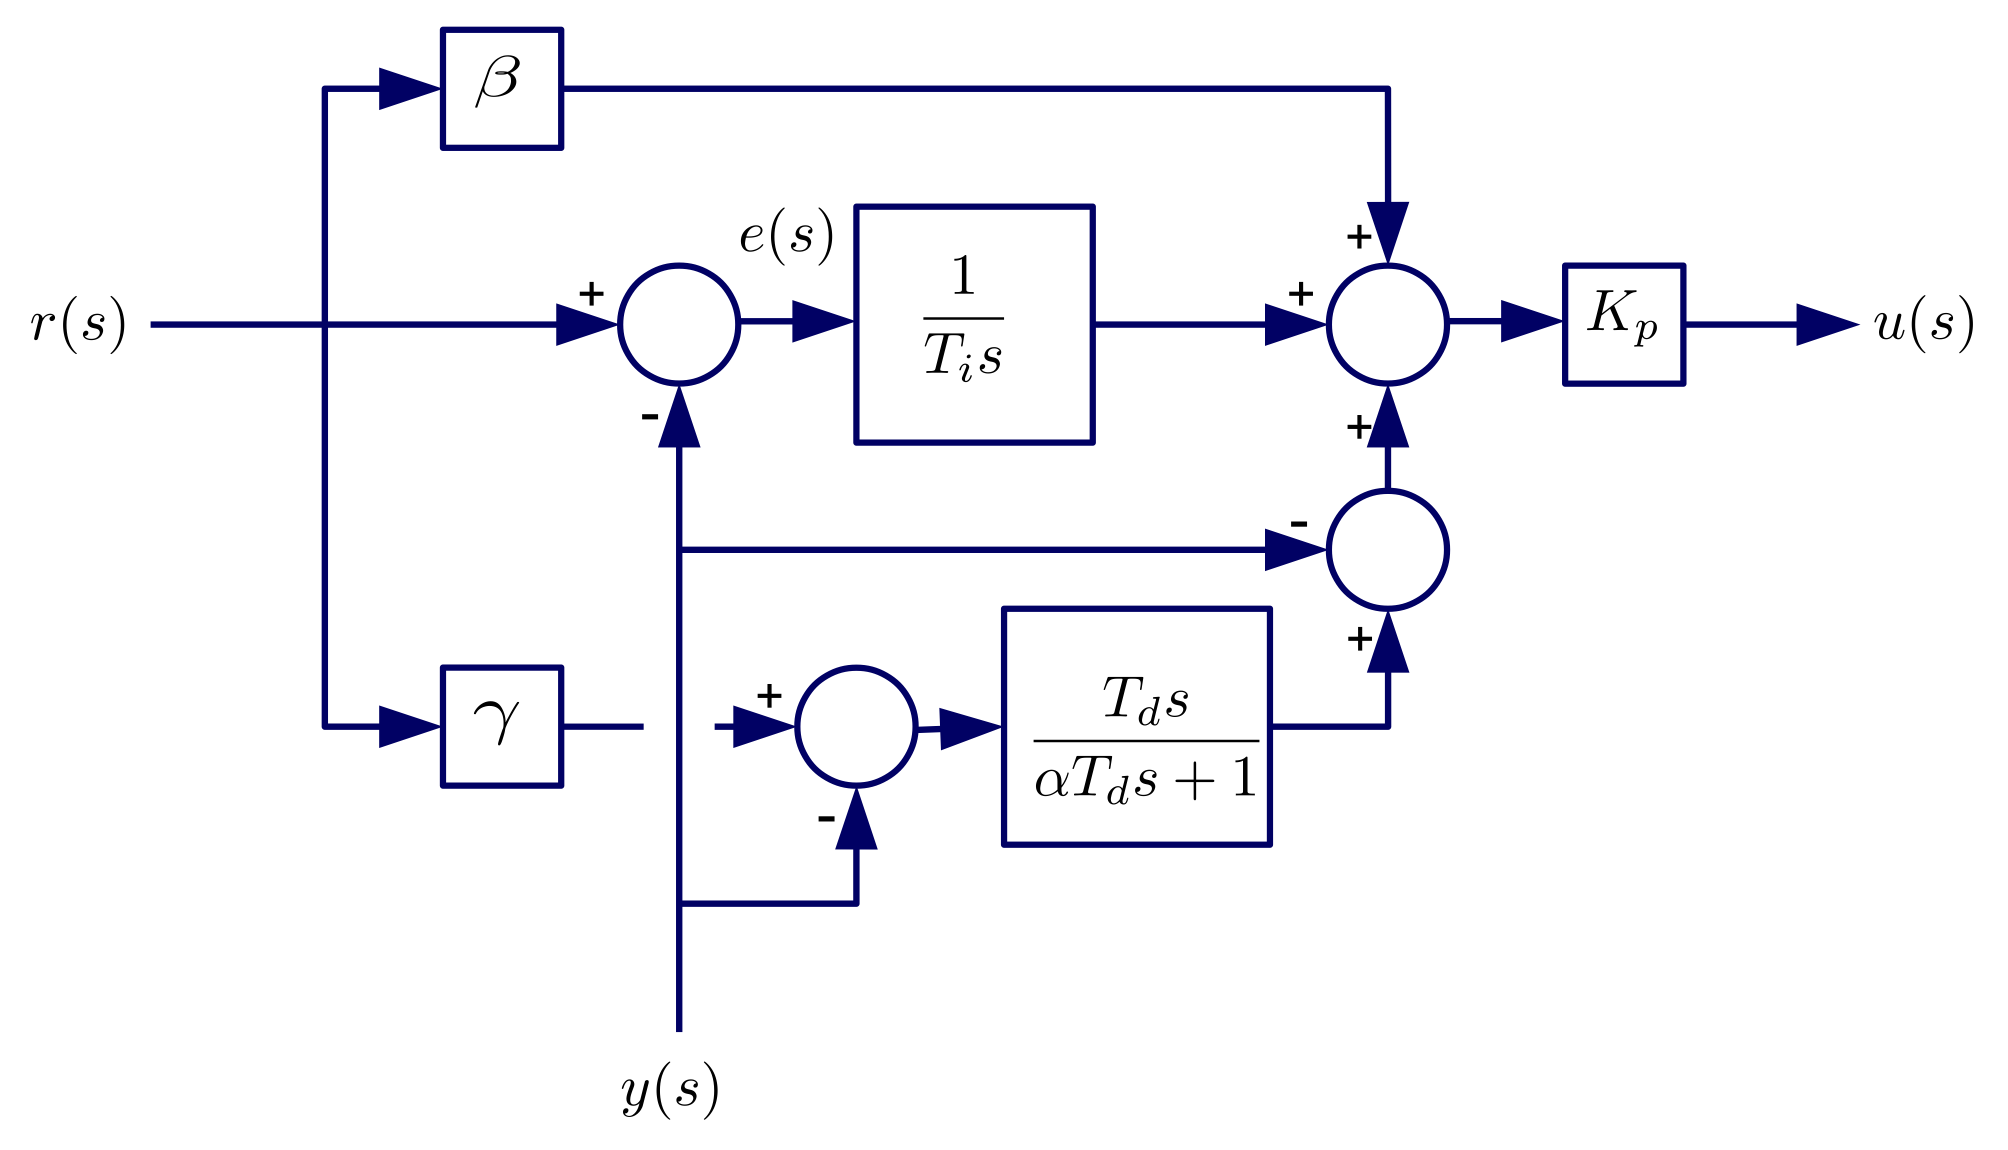
\includegraphics[width=\linewidth]{../figuras/Ch2PID_Schema} 
\caption{Two-degree-of-freedom Standard PID controller.} 
\label{Ch2fig:PID_Schema}
\end{figure}



\begin{itemize}
\item \emph{Standard PID form}: The \emph{textbook} proportional integral derivative control algorithm is the Standard PID whose output is given by the following expression~\cite{astromhagglund1995}:

\begin{equation}
    u(s)= K_p \left( 1 + \frac{1}{T_i s} + \frac{T_d s}{\alpha T_d s+1} \right ) e(s)
    \label{eq:PIDstandard}
\end{equation}

\item \emph{Parallel PID form}: The parallel or \emph{independent gains} PID control algorithm is

\begin{equation}
	u(s) =  \left( K_p + \frac{K_i}{s}+ \frac{K_d s}{\alpha_p K_d s+1}\right) e(s)
\end{equation}

\noindent where each control action has its own independent gain. The gains of the parallel form can be easily related to the gains for the standard form. Whereas the proportional gain is the same, for the integral and derivative gains we have:

\begin{equation}
K_i=\frac{K_p}{T_i} \hspace{2cm}  K_d=K_pT_d 
\end{equation} 

\item \emph{Series PID form}: The  series or \emph{interacting} implementation of the PID algorithm corresponds to the serial connection of a PI and a PD controller. The resulting transfer function is

\begin{equation}
	u(s) = K'_p \left( \frac{T'_i+1}{T'_i s}\right) \left(\frac{T'_d s + 1}{\alpha' T'_d s +1}\right)e(s)
\end{equation}

In this case, parameters are denoted with a prime in order to distinguish them from the standard form ones. As a first difference with the previous formulations, it can be observed that with the series form we can not have complex conjugate zeros. If, for simplicity, we assume the ideal case, $\alpha=\alpha'=0$, a series PID controller equivalent to a Standard one would exists only for $T_i \ge 4 T_d$ (this ensures the Standard PID does not have complex conjugate zeros).

\item \emph{Filtered ideal PID form}: This formulation arises also as an alternative to the mentioned implementation problems with the ideal derivative. In this case, the overall control variable is filtered:

\begin{equation}
	u(s) =  K^*_p \left(1+ \frac{1}{T^*_i s} + T^*_d s  \right) \left(\frac{1}{T_f s+1}\right) e(s)	
\end{equation} 

In this case, parameters are denoted with a star in order to distinguish them from the standard and series form ones. Notice that the controller variable filter introduces the filter time constant $T_f$ as an additional controller parameter. This fact will make the relationship of this controller formulation parameters with the previous ones not so straightforward. It will be presented later on on a more general framework. 
\end{itemize}



\subsection{Reference Processing and 2-DoF PID}
\label{sec:3.2}

The previous PID controller formulations can be improved by introducing some considerations on the processing of the reference signal. The first one is regarding the effect of a step change, $\Delta r$ in the derivative part. Considering, for simplicity, a PD controller, an instantaneous change $\Delta u$ in the control signal will be generated. This instantaneous change will be of magnitude

\begin{equation}
\Delta u = K_p \left ( 1 +\frac{1}{\alpha} \right ) \Delta r \xrightarrow[\alpha=0.1]{}\Delta u = 11 K_p \Delta r
\end{equation} 

This is known as the \emph{derivative kick}. In order to avoid this, it is suggested to feed the derivative with just the output signal.  In this case, the PD controller will take the form

\begin{equation}
u(s)=K_p e(s) - K_p\frac{T_ds}{\alpha T_d s+1} y(s)
\end{equation}

Along the same lines as with the derivative term, a sudden change of magnitude $\Delta r$ in the reference signal generates an instantaneous change $\Delta u$ in the control signal given by $\Delta u = K_p \Delta r$. Therefore, for a relatively high controller gain an excessively abrupt change in the actuator may be demanded. As this is an undesirable feature, the reference signal, in the proportional control action, is recommended to be scaled by a factor $\beta$ known as the \emph{set-point weighting} factor.  The proportional part of the controller is therefore rewritten as

\begin{equation}
u(s)=K_p(\beta r(s) - y(s))
\end{equation}

By choosing $\beta < 1$, the control signal instantaneous change can be scaled down to $\Delta u = K_p \beta \Delta r$  without the need to reduce the controller gain. 

When the \emph{set-point weighting} factor is considered into the PID controller implementation, the resulting controller is said to have two-degrees-of-freedom (2-DoF) as a different processing of the reference and feedback signal is allowed. In such case, the 2-DoF versions of the previously presented PID controller formulations, also considering the avoiding of the derivative kick, results as:

\subsection{2-DoF PID Controller Algorithms Conversion}
As it can be observed from the presented PID formulations, whereas the reference controller aspect $C_r(s)$ takes the same form in all formulations, it is the feedback part $C_y(s)$  that prevents a direct translation of the controller parameters from one formulation to another. This is important because some of the existing tuning rules have been conceived for a specific PID formulation. Due to the possibility that the PID algorithm of the controller to tune be different to the one considered by the tuning rule to use, it is necessary to have conversion relations to obtain ``equivalent'' parameters between two or more of them~\cite{alfaroetfa2012-2} WEE. In what follows, we present conversion formulae to get the controller parameters for one specific PID formulation starting from the parameters got for another different one. In order to be as general as possible, the conversion formulae is presented for the more generic 2-DoF PID controller formulations just presented above.


\section{Normalised Representations}
\label{sec:3}

The design approach that is to be presented in the following chapters is applied to controlled processes represented by stable over-damped models. These models encompass from first order to double pole stable models. For control system performance analysis and controller tuning it is convenient to work with dimensionless parameters to made it non dependent on the controlled process time scale and gain. Therefore in this section the process model as well as controller transfer functions to be considered will rewritten in their normalised form in terms of dimensionless parameters.  Therefore, in this book, all the results are based on normalised transfer function models as well as the corresponding normalized controller parameters. In this way we ensure that controller design is consistent from the point of view of being aplicable to all transfer function models equivalent to the normalised one but to a time-scaling.  An additional advantage is that the number of process model transfer function do have one parameter less.\\

\subsection{Process Model Normalisation}
\label{sec:3.2}

The \emph{over-damped} controlled process (first- and second-order) are represented by a linear model given by the transfer function presented in (\ref{Ch2eq:SOPTD})

\begin{equation}
	P(s) = \frac{K \me^{-L s}}{(T s+1)(a T s+1)}, \ \ \theta_p=\left\{K, T, a, L \right\}, 
\end{equation}

\noindent where $K$ is the model gain, $T$ the main time constant, $a$ the ratio of the two time constants ($0 \leq a \leq 1.0$), and $L$ the dead-time.\\

Using the controlled process model gain $K$, and time constant $T$, as well as the transformation $\hat s \doteq T s$, the controlled process \eqref{Ch2eq:SOPTD} can be expressed in normalised form as follows:
\begin{equation}
	\hat P(\hat s) = \frac{\me^{-\tau_L \hat s}}{(\hat s +1)(a \hat s +1)}, \ \ \tau_L \doteq \frac{L}{T}, 
	\label{Ch2eq:SOPTD_n}
\end{equation}

\noindent where $\tau_L$ is the normalised (dimensionless) dead-time.\\

The over-damped second-order plus dead-time (SOPDT) \eqref{Ch2eq:SOPTD_n} model has two normalised parameters, $\hat{\theta}_p = \{a, \tau_L\}$.  For the particular case of the first-order plus dead-time (FOPDT) model ($a=0$) it has only one, $\hat{\theta}_p = \tau_L$. Using the same procedure normalised models are obtained for the other processes.\\


\subsection{Controller Normalisation}
\label{sec:3.3}

Regarding the controller, to consider the control retransfer function alone does not make sense. It has to be considered in conjunction with the process model transfer function to be controlled. Therefore, according to the normalisation of the process model, the controlled transfer function has also to be scaled. This will define the normalised controller parameters. Next we consider the normalization of the \emph{Standard 2DoF PID controller} $PID_2$ from where the normalized parameters of other 2DoF PID control algorithms can be found.

For example, the output equation of the normalized version of the \emph{Standard 2DoF PID controller} $PID_2$ in \eqref{eq:PIDstandard}, with the $\hat s \doteq T s$ transformation, is given by
\begin{equation}
	u(\hat s) = \kappa_p \left\{\beta r(\hat s)-y(\hat s) + \frac{1}{\tau_i \hat s} \left[r(\hat s)-y(\hat s)\right] - \left(\frac{\tau_d \hat s}{\alpha \tau_d \hat s+1}\right) y(\hat s)\right\},
\end{equation}

\noindent with parameters $\hat{\theta}_c = \left\{\kappa_p, \tau_i, \tau_d, \alpha, \beta \right\}$. Therefore,  for \emph{over-damped first-} and \emph{second-order plus dead-time},  models, using the corresponding model parameters the associated $PID_2$ controllers parameters can be expressed in normalised form as follows:

\begin{equation}
	\kappa_p \doteq K K_p, \ \ \tau_i \doteq \frac{T_i}{T}, \ \ \tau_d \doteq \frac{T_d}{T} 
	\label{Ch2eq:PIDNormalized}
\end{equation}

In case the controller is implemented as a \emph{PID Parallel controller} the corresponding normalized parameters are:
\begin{equation}
	\kappa_p \doteq K K_p, \ \ \kappa_i \doteq K K_i T, \ \ \kappa_d \doteq \frac{K K_d}{T}.	
\end{equation}



\chapter{PID Controller Considerations}
\label{chap:PIDControllerDesign}

\section{Control System Evaluation Metrics}
To do
\subsection{Performance}
To do
\subsection{Robustness}
To do
\subsection{Input Usage}
To do
%

\section{Control System Tradeoffs}
To do
\subsection{Servo vs. Regulation}
To do
\subsection{Performance vs. Robustness}
To do
\subsection{Input vs. Output Disturbances}
To do
\chapter{PID Controller Design}

\section{PID Controller Tuning}
The appropriate selection of the tuning parameters is one of the most important steps in the definition of a PID based control loop. This is known as the PID tuning. The selection of the PID controller parameters should be made according to the available knowledge of the process dynamics and stated performance specifications in terms of tracking and disturbance attenuation as well as desired robustness. One of the aspects that makes PID control specially appealing is the clear physical meaning associated to each one of its parameters. \\

Numerous studies have been made to develop assignment rules to specify PID parameters on the basis of characteristics of the process being controlled. The collected information about the process to be controlled can, in one form or another be assimilated to a model of the process. This can be referred either as a parametric process model (or, in other words, a form suitable for analyzing and simulating the closed-loop system), or concrete process data and/or measurements that in a suitable way can be directly employed to determine the PID controller parameters. There are many representative sources that can be consulted for details on a wide variety of alternative tuning rules  \cite{odwyer2006}, \cite{VilanovaBook2012}. \\

In what follows, a short presentation of the most usual existing methods for PID tuning are presented. The presentation will not be deep into details because it is not the purpose of this book to explore existing tuning approaches, material that, on the other hand, can be accessed on numerous sources.  However, it is important not to forget the existing panorama and main features of existing approaches, This will make possible, in the next section, to better understand the formulation of the PID tuning problem as a multiobjective optimization problem.

\subsection{Analytical Tuning Methods}

These approaches allow a specification of a desired closed-loop time response. This desired closed-loop behavior can take the form of desired poles for the closed-loop behavior, or a reference model the closed-loop system should try to mimic.  These approaches were originated by the early works on algebraic controller design (of course in a more generic setting, not just for PID controllers) by \cite{ragazzini1958}. There are different approaches for doing that; some of them place only the closed loop poles, others also shape the zeros. In contrast, by using conventional PID controller, it may not be possible to place all of the poles, so only the dominant pole is placed for this scenario. The design notion in this class of designs is based on re-assigning the system's poles with faster modes. The drawback, however, is that some modes may become uncontrollable due to pole/zero cancellation and the performance degrades if they become excited.


The introduction of ideas on algebraic design, gave rise to the so called \emph{$\lambda$-tuning} or  Dahlin method \cite{dahlin68}. It is straightforward to see that for FOPTD and  SOPTD models, PI and PID
controllers can help achieve the desired performance. The number of poles that can be placed is equal to the number of controller parameters. Therefore these techniques can be used for process models with the maximum order of 2 if a PID controller is selected. This method, in turn, is closely related to the Smith predictor and the design method based on Internal Model Control (IMC) \cite{riveraetall86}.  It is worth a special mention the fact that, for a FOPTD process, the IMC controller takes the form of a PI or a PID controller depending on the rational approximation used for the time delay.  These approaches, however, use cancellation of the poles of the process, which may lead to quite undesirable responses to load disturbances, especially for processes with very large time constants. In \cite{chien90} a modification is presented  that does not cancel the poles of the process, while \cite{Skogestad2003}, presents a variation of the IMC controller, applied to PI and PID controller tuning, denominated SIMC, in which the cancellation is avoided by means of a redefinition of the integral mode for the cases of systems dominated by large time constants. 

In 2002,  Lee and Seborg,\cite{chenseborg2002} proposed a modification of the direct synthesis method adapted to disturbance rejection instead of set-point change. Tuning rules are provided for a wide range of process models. Following these lines, in 2007  Shamsuzzoha and Lee \cite{shamsu2008}, reported that IMC demonstrates sluggish disturbance rejection, especially when the deadtime to time constant ratio is small. To alleviate this problem they proposed an IMC-PID tuning method for improved disturbance rejection.

One of the advantages of IMC is the introduction of the desired closed loop time constant which can be used by operators to manipulate the degree of robustness. In 2008 Vilanova \cite{vilanovaJPC2008}  proposed a robust IMC based ISA tuning rule for set-point tracking. The tuning introduces two user defined parameters and also provides an automatic tuning rule.


\subsection{Tuning based on Minimisation of a Performance Criterions}

The methods based on the application of optimization techniques are an alternative to the analytical methods.
The basic idea is to try to capture different aspects of the desired operation in closed loop under the signature of a determined cost functional to be minimized. In \cite{corripio2001} and in \cite{shinskey.1994}, for example, controllers are  optimized with respect to integral error criteria such as the  ISE, IAE and ITAE.  However, among the
set of tuning rules in this category, ITAE is claimed to yield better performance \cite{ogatabook}. The first works in using optimization of integral criteria for deriving tuning rules where the ones of Lopez \cite{lopez1967} and Rovira \cite{Rovira1969a}   where, coming from the load disturbance based tunings of Ziegler-Nichols, tunings are provided for both load disturbance and set-point as different closed-loop operation modes. More recently, optimal tunings have been proposed \cite{arrieta2010} for a balanced operation among both modes when two degrees of freedom are not available or, when it is not clear the predominant operation mode the control system will work on.

Quite simple tuning rules, for different variants of the integral criteria are provided in \cite{zhuang1993} . The corresponding version for unstable and integrating systems is provided in In \cite{visioli2001}. More recently, thanks in part to greater accessibility to optimization routines, powerful software and computing power, there have appeared approaches of Multiobjective optimization, such as \cite{herreros2002}  and \cite{toivonen2006}, where a generic approach is presented and its application to the particular case of a PID controller exemplified. 

The application of these optimization strategies, although effective, relies on the use of fairly complex numerical routines and not results. in general, in tuning rules as a solution of the problem. Through its application, you get the controller tuning as the solution to the optimization problem. However, as presented in some recent works, by solving the optimization problem for well defined process families and by interpolating the results, it is possible to obtain tuning formulae that give the optimal PID gains based on the process parameters. 


\subsection{Tuning Rules for Robustness}

Tuning rules designed specifically to achieve a closed-loop with some robustness guarantees. Whereas there are some tuning approaches that provide tuning parameters that  affect the system robustness (this is the case, for example of IMC control) they main aim is not to ensure a robust closed-loop system. Even if their application may derive in a control system with some robustness properties, its achievement will always be indirect. On the other hand, in recent years, there has been an increasing interest in including robustness. Starting point are the well-known design strategies based on setting the gain and phase margin, initiated in \cite{astromhagglun84} that have given rise to numerous variants and extensions. In this case, the design parameter or specification is directly measuring the desired robustness for the closed-loop system. Later on, in 1995, Ho \cite{hoetal95} proposed tuning rules for PID controllers for gain and phase specifications.

As previously mentioned, it was within the IMC approach that the work of Vilanova \cite{vilanovaJPC2008} introduced robustness considerations into the formulation of the autotuning  expressions. These ideas conducted lately to a series of works \cite{alcantara2010, alcantara2013} where the robustness was explicitly considered as part of the design and by taking into account the robustness/performance tradeoff \cite{alfaroajoc12}.

The robustness idea has evolved in such a way that today it is common use to include a robustness constraint or consideration in whatever approach. One of the measures that has gained more popularity today is the maximum of the sensitivity function (commonly called $M_S$) as a reasonable robustness measure. It is also possible to distinguish between approaches that are attempting to achieve a closed-loop with a particular value of $M_S$ and more flexible approaches providing tuning rules directly parameterized by the target $M_S$ value \cite{arrieta2012}, \cite{VilanovaBook2012}. 

The robustness constraint has also been incorporated into more elaborated  methods such as the Model reference Robust Tuning (MoReRT) approach \cite{alfarojopc22}. Such method incorporates a model reference based design within an optimization procedure and with the mentioned robustness constraint. Robust tuning rules are provided for all the most common process dynamics as well as different levels of robustness. The work also allows PID formulations where the reference and output signals are filtered. The filters are considered as parts of the design \cite{alfaroiechr2013}.




%
\section{Formalization of PID tuning as a multiobjective optimization problem}
\label{sec:FormPIDMOOP}
\subsection{Cost functions and constraints selection}
\label{sec:CostFunSelec}
When dealing with \gls{pid} tuning, it is common to define a metric either to optimize the parameters, or as a measure to check how well the tuning behaves with respect to other set of parameters.

In theory, to formulate the \gls{moo} problem, any cost function may be used. However, it is common to select cost functions that are contradictory to each other, which is something that arises naturally when dealing with real designs.

For example in \cite{SabinaSanchez2017} the \gls{iae} and the total variation are used as contradictory cost functions. The total variation represents the control effort and is related to the robustness of the closed system, therefore, using these two cost functions, the compromise is made between performance and robustness. Something similar is done in \cite{Pierezan2014}, where a particle swarm optimization technique is applied to the tuning of \gls{pid} controllers for a robotic manipulator. In \cite{Zhou2018} also a two objectives optimization is done with similar cost functions, the difference consist in that a multivariable control loop is tackled at the same time using a compound weight sum of an \gls{iae} metric for three setpoints and a function related to the energy consumption based on the variation of the input variables.

The cost functions not necessarily is an integral function. For example in \cite{Abbas1995} the cost functions are the percent overshoot  and the rise time, but the authors also indicate that the settling time and the maximum controller output can be also considered. A more classical approach takes into account frequency domain measures as phase and gain margins \cite{astromhagglun84,hoetal95}. In \cite{Huang2008a} the $\cal{ H}_\infty$ norm is used in different frequency bands of different sensitivity functions to define several cost functions which are then used in a multi-objective approach.

Other authors tries to combine integral cost functions with other time domain measures, as in \cite{Chiha2012} where the settling time, overshoot, rise time, \gls{iae}, \gls{ise} and \gls{itae} are taken into account in a weighted sum and optimized using an Ant Colony algorithm approach.

Definitively, the selection of the cost function is widely open and it entirely depends on the necessity of the task at hand. According to \cite{Shinskey2002}, the main objective of a process controller is to mitigate the effects of load of disturbances, setpoint changes are considered of secondary importance. The same authors states that: \begin{quote}
	``minimum \gls{iae} is a preferred criterion that includes integral error and penalizes continued cycling. Minimum-\gls{iae} tuning also tends to be consistent with minimum error.''
\end{quote}
%

Following this reasoning, in this work we propose to use integral cost functions to measure input and output disturbances and setpoint changes in a multi-objective framework, taking the maximum sensitivity as a constraint to find the optimal controller tuning in a Pareto sense.

The controller is considered to be a \gls{2dof} \gls{pid} controller. Even with this topology, the cost functions that results of considering all three sources of disturbances are contradictory among them because minimizing one of them does not minimize the other functions, in fact you may find that the optimal controller for one cost function yields to the maximum value of other function. These details are covered in Section~\ref{sec:MOOPForm} where the multi-objective framework is stated.

\subsection{PID tuning problem formulation for integral cost functions}
\label{sec:CostProbPID}
A feedback control system like the one shown in %
\begin{figure}[tb]
	\centering
	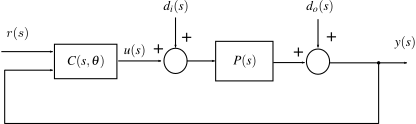
\includegraphics[width=\columnwidth]{Ch4bloques}%pretex=\scriptsize,
	\caption{Feedback control loop.}% 
	\label{fig:bloques}%
\end{figure}
%
Figure~\ref{fig:bloques}, also called closed-loop control system, is designed to keep certain relationship between the process output $y(s)$ and the reference input $r(s)$. For such task, the difference between those signal is used to compute the control signal $u(s)$ needed in order to achieve $y(s)=r(s)$. 

In Figure.~\ref{fig:bloques}, $C(s,\bm{\theta})$ is the \gls{2dof} \gls{pid} controller with parameters:
\begin{equation*}
\bm{\theta}=\left[	\begin{tabular}{cccc} \gls{kp} & \gls{ti} & \gls{td} & \gls{beta}	\end{tabular}\right]^T
\end{equation*}
%
with \gls{kp} the proportional gain, \gls{ti} the integral time constant, \gls{td} is the derivative time constant, \gls{beta} the weight on the reference signal. \gls{plan} represents the controlled process, modeled as a \gls{soptd} plant, with a transfer function of the form:
\begin{equation}  %inclusión de ecuaciones
P(s) =  \frac{K e^{-Ls}}{(T s+1)(a T s+1)},
\label{eq:plantaX}
\end{equation}
%
where \gls{k}, \gls{l} and \gls{t}, correspond to the static gain, the time delay and main time constant respectively. The other pole of the system is represented with a time constant that is fraction of $T$, therefore $0 \leq a \leq 1$. \gls{di} represent the input disturbance while \gls{do} is the output disturbance.

%El diagrama de bloques de un controlador PI de dos grados de libertad se muestra en la Figura \ref{fig:controlador}. 
%
The relationship between the control signal, the reference and the process output is given by:
%
\begin{equation}  %inclusión de ecuaciones
\gls{u} = \gls{contr} \gls{r} - \gls{conty} \gls{y},
\label{us}
\end{equation}
%
where the part applied to the reference signal is given by:
%
\begin{equation}  %inclusión de ecuaciones
\gls{contr}=  \gls{kp}\left({\gls{beta} + \frac{1}{\gls{ti} s}+ \gls{gamma} \frac{\gls{td} s}{\gls{alpha} \gls{td} s +1}}\right),
\label{eq:cr}
\end{equation}
%
and the part applied to the process output is:
%
\begin{equation}  %inclusión de ecuaciones
\gls{conty}=  \gls{kp}\left({1 + \frac{1}{\gls{ti} s}+\frac{\gls{td} s}{\gls{alpha} \gls{td} s +1} }\right).
\label{eq:cy}
\end{equation}

It is common to set $\gls{alpha}=0.1$ and $\gls{gamma}=0$. For this reason, the controller parameter vector is give as $\gls{theta}=[\begin{tabular}{cccc} \gls{kp} & \gls{ti} & \gls{td} &\gls{beta} \end{tabular}]^T$. A detailed depiction of the controller transfer function is presented in 
\begin{figure}[tb]
	\centering
	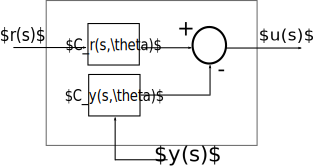
\includegraphics[width=0.7\columnwidth]{Ch4controlador}
	\caption{Representation of the \gls{2dof} controller.}
	\label{fig:Ch4controlador}
\end{figure}
%
Figure~\ref{fig:Ch4controlador}.

To simplify the analysis, the model of the controlled process is normalized:
%
\begin{equation*}
\hat{s}= Ts, \ \tau_0=  \displaystyle\frac{L}{T}, \ \tau_i=  \displaystyle\frac{T_i}{T}, \ \tau_d = \frac{T_d}{T}, \ \kappa_p= K_p K.
\end{equation*}  %inclusión de ecuaciones

Then the normalized parameters of the controller become $\bm{\theta}=\left[\kappa, \tau_i, \tau_d, \beta\right]^T$.
%
and the response of the controlled system is computed as: 
%%
\begin{equation} 
 y(\hat{s})= y_r(\hat{s}) + y_{di}(\hat{s}) + y_{do}(\hat{s}),
\label{ys}
\end{equation}
%
where $y_r(\hat{s})$, is the output response to a change in the setpoint $r(\hat{s})$, $y_{di}(\hat{s})$ is the response to a change in the input disturbance signal $d_i(s)$ and $y_{do}(\hat{s})$ is the response to a change in the ouput disturbace signal $d_o(s)$. From Figure~\ref{fig:bloques} and Figure~\ref{fig:Ch4controlador}, these signals can be computed as:
%
\begin{align*}
 y_r(\hat{s}) &= \frac{P(\hat{s}) C_r(\hat{s},\bm{\theta}) }{1 + P(\hat{s}) C_y(\hat{s},\bm{\theta})} r(\hat{s})\\
y_{di}(\hat{s}) &=  \frac{C_r(\hat{s},\bm{\theta})}{1 + P(\hat{s}) C_y(\hat{s},\bm{\theta})} d_i(\hat{s}) \\%
y_{do}(\hat{s}) &= \frac{1}{1 + P(\hat{s}) C_y(\hat{s},\bm{\theta})} {d_o(\hat{s})}
\label{ytot}
\end{align*}

%Dada \eqref{ys}, la respuesta de salida del lazo cerrado ante un cambio en el valor deseado puede ser ajustada a través del controlador de valor deseado $C_r(\hat{s},\theta)$, independientemente de cambios en la perturbación de entrada o en la de salida. Los parámetros de $C_r(\hat{s},\theta)$ y $C_y(\hat{s},\theta)$ son los mismos con un grado de libertad \cite{apuntescontrol}.

Robustness is an indication of the relative stability of the controlled system and it measure the ability of the controller to keep the closed loop stable despite the variation in the process dynamics. A metric of the degree of relative stability is the maximum sensitivity \gls{ms} given by:
%
\begin{equation}  %inclusión de ecuaciones
\gls{ms}=  \max_\omega \left\{ \frac{1}{\left |{1 + C_y(j\omega ) P(j\omega )}\right |}\right\} 
\label{Ms}
\end{equation}

The recommended value range is  $1.2\leq \gls{ms} \leq 2.0$.

As it is widely established, the controller tuning can be solved as a multi-objective optimization problem~\cite{Gambier2007}. One common indicator of performance, is the \gls{iae} given by:
%
\begin{equation}  %inclusión de ecuaciones
J(\bm{\theta})=\int_0^\infty \left |{e(t,\bm{\theta})}\right | dt.
\label{IAE}
\end{equation}

The error signal $e(t, \bm{\theta})$ it is calculated using:
%
\begin{equation}  %inclusión de ecuaciones
e(t,\bm{\theta})=r(t)-y(t,\bm{\theta}).
\label{error}
\end{equation}

When \eqref{IAE} is computed for a step change in the reference signal, the cost function becomes $J_r(\bm{\theta})$; for an input disturbance response, the function is defined as $J_{di}(\bm{\theta})$ and finally, for an output disturbance response, the cost function is named as $J_{do}(\bm{\theta})$.

When the output of the plant is disturbed only by the step change in $d_i(s)$, the error signal then becomes:
\begin{equation}  %inclusión de ecuaciones
e_d(t)=-y_{di}(t)
\label{per}.
\end{equation}

And then, the cost function $J_{di}(\bm{\theta})$ is computed as:
\begin{equation}  %inclusión de ecuaciones
J_{di}(\bm{\theta})= \int_0^\infty  \left |-{y_{di}(t,\bm{\theta})}\right | dt,
\label{perin}
\end{equation}

On the other hand, if the disturbance comes only from a step signal in $d_o(s)$, the cost function that has to be computed is $J_{do}(\bm{\theta})$ as:
%
\begin{equation}  %inclusión de ecuaciones
J_{do}(\bm{\theta})= \int_0^\infty  \left |-{y_{do}(t,\bm{\theta})}\right | dt.
\label{perout}
\end{equation}	
%

Finally, if the setpoint is the only source of disturbance for the plant, the corresponding cost function $J_r(\bm{\theta})$ is computed as:
\begin{equation}  %inclusión de ecuaciones
J_r(\bm{\theta})=\int_0^\infty \left |r(t)-y_r(t,\bm{\theta})\right | dt.
\label{eq:Jr}
\end{equation}
%

The problem of minimizing $J_r(\bm{\theta})$, $J_{di}(\bm{\theta})$ and $J_{do}(\bm{\theta})$ at the same time can be posed as a \gls{moo} problem. In addition, since in an industrial environment the robustness is very important, the obtained parameters are constrained to always satisfy  $\gls{ms} \leq M_{s,max}$, where $M_{s,max}$ is the allowed limit of the maximum sensitivity. The combined cost function (vector of cost functions) then becomes:
%
\begin{equation}  %inclusión de ecuaciones
\textbf{J}(\bm{\theta})=\left[J_{di}(\bm{\theta}), J_{do}(\bm{\theta}), J_{r}(\bm{\theta})\right]^T,
\label{eq:Jtotal}
\end{equation}
%
and solved by finding all possible optimal solutions of:
%
\begin{equation}  %inclusión de ecuaciones
\begin{gathered}
\textbf{J}(\bm{\theta}^*) = \min_{\bm{\theta}} \textbf{J}(\bm{\theta}),\\
\text{s.t.} \quad  M_s \leq M_{s,max}
\end{gathered}
\label{eq:probmoo}
\end{equation}

In general, it is not possible to find a set of parameters $\bm{\theta}$ that minimizes all those three functions at the same time. Such impossible point where all the cost functions are optimal is called the utopia point. As it names states, the utopia point is impossible to reach because optimizing one of the cost function always produce a degradation in the other remaining functions.

The particular cases that are  the closest to the utopia point, are part of what is called the Pareto frontier. This set of possible solutions are considered to be equally optimal because there is no possibility to improve one of the functions without degrading the others.

This means that solvingthe solution of the control problem does not give a single solution, instead a family of optimal controller tunings are found.
\chapter{Multi-objective optimization methods}
\label{sec:Metodolgia}
\begin{refsection}
\section{Multi-objective optimization problem formulation}
\label{sec:MOOPForm}

A \gls{moop} arises when, in order to solve a given problem or design, it is necessary to optimize several cost functions at the same time. 

In general, these cost functions depend on the same variables and usually are in conflict.  In addition, they may be independent of one another, that is, the value of the variables that optimize one of the function do not necessarily optimize the other cost functions.

In those cases, given a set of cost functions:
\begin{equation}
\mathbf{F}(\xv)=\left[F_1(\xv), F_2(\xv), F_3(\xv), \ldots, F_k(\xv)\right]^T
\label{eq:functions}
\end{equation}
%
that depends on $n$ different variables $\xv=\left[x_1, x_2, \ldots, x_n \right]^T$, $x_i \in \mathbf{X}$, where $\mathbf{X}$ is the feasible decision space. The \gls{moop} may be formulated as follows \parencite{Marler2004}:%
%
\begin{subequations}%
	\begin{align}%
	&\min_\xv \mathbf{F}(\xv), \label{eq:Min01}\\ %
	&\text{s.t.}\nonumber\\%
	& \hspace{5mm} g_j(\xv) \leq 0, \qquad j=1,2,\ldots,m  \label{eq:Min02}\\ %
	& \hspace{5mm} h_l(\xv) = 0, \qquad l=1,2,\ldots,e  \label{eq:Min03}%
	\end{align}%
	\label{eq:OptProb}%
\end{subequations}%
%
where $g_j(\xv)$ is the $j$-th inequality constraint and $h_l(\xv)$ is the $l$-th equality constraint. 

In general, it is not possible to find a set of variables values that minimizes all $F$ functions. In fact, the optimization problem in \eqref{eq:OptProb} have multiple equally optimal solutions in the sense of the Pareto optimality. According to \cite{Marler2004}:
\begin{quote}
	``A point $\xv^*\in \mathbf{X}$, is Pareto optimal iff there does not exist another point, $\xv \in \mathbf{X}$, such that $\mathbf{F}(\xv)\leq\mathbf{F}(\xv^*)$, and $F_i(\xv)<F_i(\xv^*)$ for at least one function''
\end{quote}

The concept of Pareto optimality is represented in %
%
\begin{figure}
	\centering
	\includesvg[width=0.8\columnwidth]{./figuras/planoFun01}
	\caption{Function space}
	\label{fig:planoFun01}
\end{figure}
%
figure~\ref{fig:planoFun01} for a two-function multi-objective optimization. The gray area represents the feasible function space, given by the value of $F_1(\xv)$ and $F_2(\xv)$ for all $\xv \in \mathbf{X}$. From all those points, only the points in the curve from ``a'' to ``b'' (marked with a thicker dash line) are Pareto optimal because there is not another point in the feasible decision space with a lower value of $\mathbf{F}$, but there is at least one point that has a lower value for either $F_1$ or $F_2$. The curve from ``a'' to ``b'' is the Pareto front and contains all possible solutions to problem \eqref{eq:OptProb} that are Pareto optimal. These solutions are always in the edge of the feasible function space, closer to the utopia point (the ``u'' point in the figure). The utopia point is a point in the space where all the cost functions have their minimum value. As it can be seen from figure~\ref{fig:planoFun01}, this point is more likely to be outside of the feasible function space.

Points ``a'' and ``b'' are called anchor points and represent the combination of decision variables that optimizes at least one of the functions. In this case, ``a'' is the point where function $F_1(\xv)$ has its minimum value whereas ``b'' the one in which $F_2(\xv)$ has its minimum value.

Point ``N'' is called the pseudo-nadir point, and is defined as the point with the worst values of all the anchor points.
%--------------------------------------------------------------------------
%-------------------------------o-o-o--------------------------------------
%--------------------------------------------------------------------------
\section{Scalarization algorithms to find the Pareto front}
\label{sec:design-methodologies}

In general, the algorithms to find the optimal value of a function are designed to be used in a single objective paradigm. In order to be able to use the same standard algorithms with a multi-objective problem, some scalarization method has to be employed.
%
\subsection{Weighted Sum}
\label{sec:WS}
%
\gls{ws} methodology is a popular procedure to transform a \gls{moop} into a single objective problem by creating a new objective function that is the result of the aggregation of all the functions involved with certain weight for each one \parencite{Marler2004}. For example, if the two objectives to optimize are $f_{1}(\mathbf{x})$ and $f_{1}(\mathbf{x})$, the new function is given by:
\begin{equation}
F_{WS}(\mathbf{x}) = \alpha_{1WS} \hat{f}_{1}(\mathbf{x}) + \alpha_{2WS} \hat{f}_{2}(\mathbf{x}),
\label{eq:JWS}
\end{equation}
with $\alpha_{1WS} + \alpha_{2WS}=1$, and $\hat{f}_{1}(\mathbf{x})$ and $\hat{f}_{2}(\mathbf{x})$ the normalized versions of $f_{1}(\mathbf{x})$ and $f_{2}(\mathbf{x})$, respectively. One possible normalization (see \cite{Marler2004}) is given by:
\begin{equation}
\hat{f}_{1}(\mathbf{x}) = \frac{f_{1}(\mathbf{x})-\min{\left( f_{1}(\mathbf{x})\right) }}{\max{(f_{1}(\mathbf{x}))}-\min{\left( f_{1}(\mathbf{x})\right) }}.
\label{eq:NormalizedJ}
\end{equation}

With this normalization, the utopia point is moved to the origin and the maximum value of the new normalized function is 1.

The optimization problem then is written as:
\begin{equation}
\begin{gathered}
\min_{\mathbf{x}}{\; F_{WS}(\mathbf{x})}, \\
\text{s.t.} \; h(\mathbf{x})=0, \\
g(\mathbf{x}) \leq 0,
\end{gathered}
\label{eq:WSProblem}
\end{equation}
%
where $h(\mathbf{x})$ and $g(\mathbf{x})$ are the equality and inequality constraints of the original problem.

There are certain drawbacks with this approach. In first place, when \eqref{eq:JWS} is minimized for different values of $\alpha_{1WS}$ and $\alpha_{2WS}$ in order to obtain the Pareto front, an even distribution of the weights does not assure an even distribution of the points in the front. Also, with \gls{ws} it is not possible to obtain Pareto points in the non-convex region of the front, and therefore, not all the possible solutions can be found \parencite{Das1997}. %In order to tackle this issue, alternative problem formulation have been proposed in the literature in order to obtain the Pareto front \parencite{Marler2004}.
%
%
\subsection{Normal Boundary Intersection}
\label{sec:NBI}
%
The \gls{nbi} is a variation in the way that the \gls{moop} is posed as a single objective optimization problem, in order to obtained an even spaced Pareto front \parencite{Das1998}. In %
%
\begin{figure}%
	\centering
	\includesvg[pretex=\scriptsize, width=0.8\columnwidth]{./figuras/NBI}%
	\caption{\gls{nbi} optimization method.}%
	\label{fig:NBI}%
\end{figure}
%
figure~\ref{fig:NBI}, a representation of the method is shown for two normalized objective functions. If the utopia plane (the plane that contains the anchor points, in the case of a bi-objective problem, the straight line that joints the anchor points) is parametrized by $\Phi\mathbf{\beta}$, where $\Phi(:,i)=\mathbf{F}(\mathbf{x}_i^*)-\mathbf{F}(\mathbf{x}^*)$, $\mathbf{F}(\mathbf{x}_i^*)$ is the value of the multi-objective function evaluated in the $i$th anchor point, $\mathbf{F}(\mathbf{x}^*)$ is the value of the function at the utopia point, and $\beta$ is chosen as:
\begin{equation}
\beta=
\left[\begin{tabular}{c}
$\alpha_{1NBI}$ \\ $\alpha_{2NBI}$
\end{tabular}\right],
\label{eq:Beta}
\end{equation}
with $\alpha_{1NBI}+\alpha_{2NBI}=1$.

Then, the idea behind the \gls{nbi} method is to find the maximum distance from the utopia plane towards the utopia point (with direction $\hat{\mathbf{n}}$) that is normal (or pseudo normal as proposed in \parencite{Das1998}) to the utopia plane. In other words, the objective is to find the border of the feasible region that is closer to the utopia point, but, by varying the parameter $\beta$ in a systematic way, it is possible to obtain an even spaced realization of the Pareto front. 

The problem then is posed as follows:%
%
\begin{equation}
\begin{gathered}
\max_{\xv,v}{\;v}, \\
\text{s.t.} \ \Phi \boldsymbol{\beta} + v \hat{\mathbf{n}} = \mathbf{F}(\xv),\\
h(\xv)=0, \\
g(\xv) \leq 0.
\end{gathered}
\label{eq:NBIProblem}
\end{equation}%

In practice, the \gls{nbi} method adds an equality constraint to the problem in such a way that, by maximizing a new variable $v$ (which represents the distance from the utopia plane towards the utopia point), the border that is closer to the utopia point is found. Depending on the shape of the frontier, it is possible that the \gls{nbi} finds points that are not Pareto optimal but belong to the edge of the feasible space. These points can be useful to have a better idea of the convexity (or lack thereof) of the Pareto front.
%
%
\subsection{Normalized Normal Constraint}
\label{sec:NNC}
The \gls{nnc} is presented in \cite{Messac2003} and is intended to improve the results of the \gls{nbi} by formulating the optimization problem only with inequality constraints and by filtering all the non-Pareto optimal points. The main idea of the methodology is presented in
%
\begin{figure}%
	\centering
	\includesvg[pretex=\scriptsize, width=0.8\columnwidth]{./figuras/NNC}%
	\caption{NNC optimization method.}%
	\label{fig:NNC}%
\end{figure}
%
figure~\ref{fig:NNC}: the utopia plane is parameterized in a similar way as the \gls{nbi} but, instead of constraining the points to be within a line, the new constrained feasible region is constructed with the original feasible region and a line that is normal to the utopia plane. With this new feasible region it is only required to minimize one of the functions (e.g. $f_{1}$) in order to find the Pareto front.

By varying the parameter $\bar{\mathbf{X}}_{pj}$ along the utopia plane, it is possible to find an even spaced front. $\bar{\mathbf{X}}_{pj}$ is computed as%
%
\begin{equation}
\bar{\mathbf{X}}_{pj}= \alpha_{1NNC} \mathbf{\hat{F}}(\mathbf{x}_1^*)+\alpha_{2NNC} \mathbf{\hat{F}}(\mathbf{x}_2^*).
\label{eq:Xpj}
\end{equation}%
%
with $\alpha_{1NNC}+\alpha_{2NNC}=1$ and where $\mathbf{\hat{F}}(\mathbf{x}_1^*)$ is the first anchor point and $\mathbf{\hat{F}}(\mathbf{x}_2^*)$ is the second. The methodology can be extended to higher dimensions.

The optimization problem can be written as follows:
%
\begin{equation}
\begin{gathered}
\min_{\mathbf{x}}{\; \hat{f}_{1}(\mathbf{x})}, \\
\text{s.t.} \ \bar{\mathbf{N}}_1^T \left(\hat{\mathbf{F}}(\mathbf{x})-\bar{\mathbf{X}}_{pj}\right) \leq 0,\\
h(\mathbf{x})=0, \\
g(\mathbf{x}) \leq 0,
\end{gathered}
\label{eq:NNCProblem}
\end{equation}
%
where $\bar{\mathbf{N}}_1$ is the vector that contains the direction of the utopia plane.
%
\subsection{Enhanced Normalized Normal Constraint}
\label{sec:ENNC}
The \gls{ennc} \parencite{Sanchis2008}, is a new perspective of the original \gls{nnc} method. Implicitly, the \gls{nnc} method supposes that in each anchor point, the other functions that are not optimal, have their worst value. For a two functions optimization, this is always the case; however for more than two functions this supposition is not true in general. The \gls{ennc} method redefines the anchor points in such a way that the supposition of the \gls{nnc} holds true, and then the same method may be used. Other advantage of the \gls{ennc} is that it is possible to expand the explored regions of the problem, given a better representation of the Pareto front.

The new anchor points (called pseudo anchor points) are defined as:
\begin{equation}
F_i^{**} = \left[
\begin{tabular}{cccccc}
$f_1^N$ & $f_2^N$ & $\cdots$ & $f_i^{*}$ & $\cdots$ & $f_n^N$
\end{tabular}
\right],
\label{eq:PseudoAnchor}
\end{equation}
%
where $f_i^N$ if the value of function $f_i$ at the pseudo nadir point. The effect of this new definition is to enlarge the utopia hyper plane and scaling the functions in such a way that the Pareto front is evenly obtained while the unexplored regions of the Pareto are reduced.

The Pareto is then computed using the same methodology as in the \gls{nnc} case.
\printbibliography
\end{refsection}
\chapter{Application of the multiobjective approach}
\label{chap:ApplicationExamplesNoGUI}

\abstract{In this chapter, the \gls{moo} techniques are tested and applied to different scenarios. A comparison of the implementation of several scalarization techniques is presented. Then, a well known benchmark problem is tackled with the presented methodology and compared with different tuning methods. Finally, a LiTaO$_3$ Thin Film Deposition Process is used as a prototype for a large dead-time process and tested using a two cost function arrangement.}

\section{Comparison of the methods to obtain the Pareto front}
\label{sec:Comparison}
\subsection{Performance comparison of the scalarization methods}
In order to compare the efficiency of different linearization methods, different test were performed on the normalized process given by:
%
\begin{equation}
\hat{P}(\hat{s}) = \frac{e^{-\tau_0 \hat{s}}}{\hat{s}+1},
\label{eq:NormP}
\end{equation}
%
with values of $\tau_0$ from $0.1$ to $2$. In order to show the results, the simulations presented in this section only contains the case for $\tau_0=0.5$. The other values of $\tau_0$ give similar results.

For this particular case, the controller is supposed to be represented by the transfer function $C(s,\bm{\theta})$ given by \gls{2dof} \gls{pi} controller:
\begin{equation}
u(s) = C_r(s,\bm{\theta}) r(s) - C_y(s,\bm{\theta}) y(s),
\label{eq:2PIControl}
\end{equation}
where $C_r(s,\theta)$ is the reference controller given by the transfer function:
\begin{equation}
C_r(s,\bm{\theta})= K_p \left(\beta + \frac{1}{T_i s} \right),
\label{eq:CrControl}
\end{equation}
%
and $C_y(s,\theta)$ is the feedback controller given by the transfer function:
\begin{equation}
C_y(s,\bm{\theta})=K_p \left(1 + \frac{1}{T_i s} \right),
\label{eq:CyControl}
\end{equation}
%
The parameters $K_p$, $T_i$ and $\beta$ are as usual, the proportional gain, the integral time and the set-point weight, respectively, which can be grouped as a single vector variable denoted by $\bm{\theta}=\left[K_p,T_i,\beta\right]^{T}$.

In %
\begin{figure}[tb]%
	\centering
	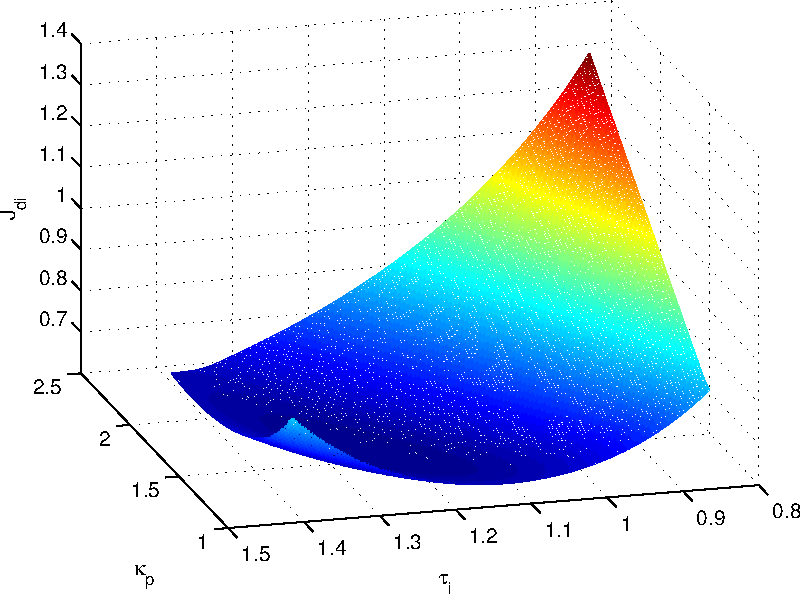
\includegraphics[width=0.8\columnwidth]{RealPareto_t0_05Jdi}%
	\caption{$J_{di}(\hat{\theta})$ function for a value of $\tau_0=0.5$.}%
	\label{fig:RealPareto_t0_05Jdi}%
\end{figure}
%
%
Figure.~\ref{fig:RealPareto_t0_05Jdi}, the cost function $J_{di}(\hat{\theta})$ is plotted as a function of $\kappa_p$ and $\tau_i$, which represent the normalized parameters of the \gls{pi} controller:
\begin{equation}
\begin{array}{c}
\kappa_p \doteq K K_p,\\
\tau_i \doteq \frac{T_i}{T}.
\end{array}
\label{eq:NormContrParam}
\end{equation}

From Figure~\ref{fig:RealPareto_t0_05Jdi}, it can be concluded that the cost function $J_{di}$ is rather convex, and very flat close to its minimal value. The graph in Fig.~\ref{fig:RealPareto_t0_05Jdi} was plotted with ten thousand controller tunings of the controller taking the optimal tuning of $J_{di}(\theta)$ and $J_{do}(\theta)$ as central points. The computation time to obtain this set of data was in the range of hours. In Fig.~\ref{fig:RealParetot0_05}, the complete set of points is plotted in the objective functions plane with the corresponding Pareto front highlighted. The points that represent the Pareto front represents only 3\% of all the points plotted in that figure. This fact shows the necessity to use some scalarization methods like \gls{nbi} or \gls{nnc} in order to obtain only the front, without the need to compute points that will be dismissed later in the process.
%
\begin{figure}[tb]%
\centering
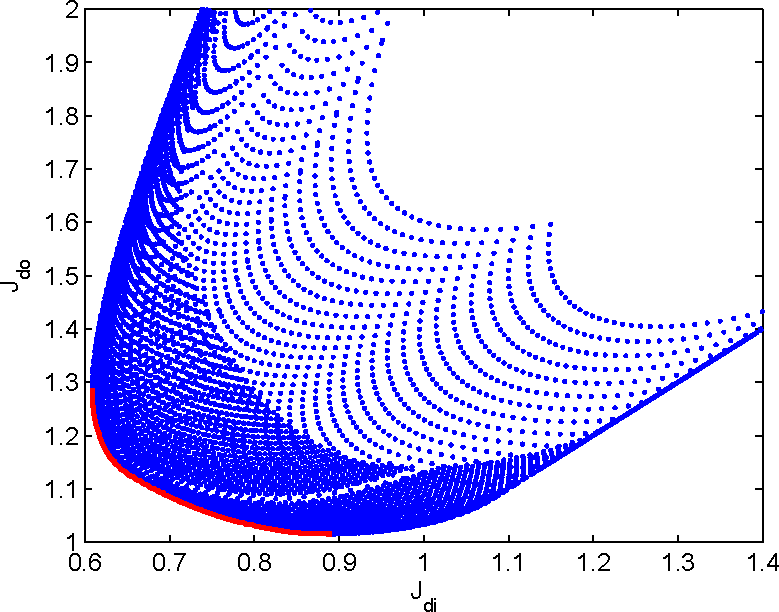
\includegraphics[width=0.8\columnwidth]{RealParetot0_05} %
\caption{Pareto front obtained directly from a ten thousand points data set for \eqref{eq:NormP} with $\tau_0=0.5$.}%
\label{fig:RealParetot0_05}%
\end{figure}

%The Pareto front was obtained with 50 points using the WS, NBI, NNC and LRC methods. 
In Fig.~\ref{fig:ParetoWSt0_05}, the result using \gls{ws} is presented. The solid line represents the real Pareto front and the points marked with a plus sign correspond to the obtained values. As it can be seen, all the points obtained with the \gls{ws} method are Pareto optimal, however its distribution is not evenly spaced and are grouped for low values of $J_{di}(\theta)$. This is expected since the shape of the Pareto front does not correspond to the relation needed to obtain an even spaced front with an even spaced parametrization of $\alpha_1$ and $\alpha_2$ as presented in \cite{Das1997}.
%
\begin{figure}[tb]%
\centering
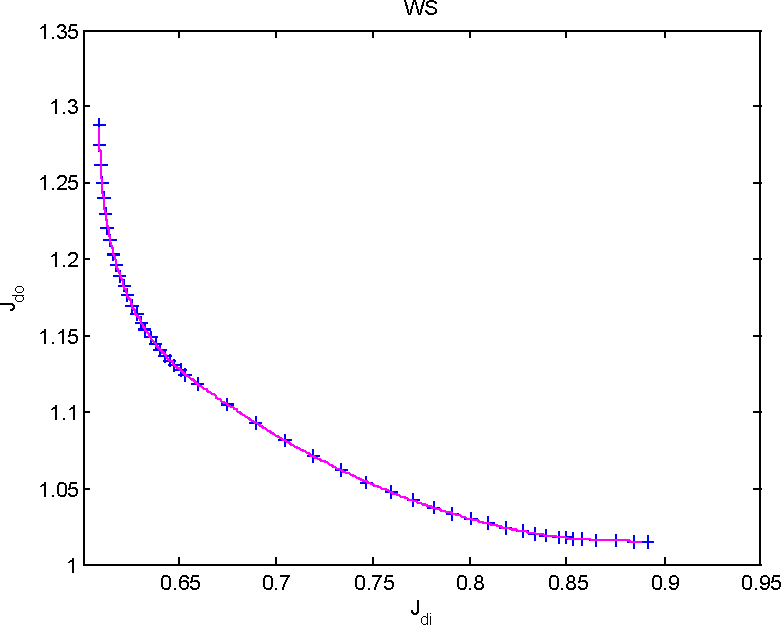
\includegraphics[width=0.8\columnwidth]{ParetoWSt0_05}%
\caption{Pareto front obtained with \gls{ws} method and $\tau_0=0.5$.}%
\label{fig:ParetoWSt0_05}%
\end{figure}

The result for \gls{nbi} method is presented in Fig.~\ref{fig:ParetoNBIt0_05}. As it can be seen, the frontier obtained with this method is evenly spaced. It is important to note that the method finds different Pareto optimal points than the \gls{ws} method
%
\begin{figure}[tb]%
\centering
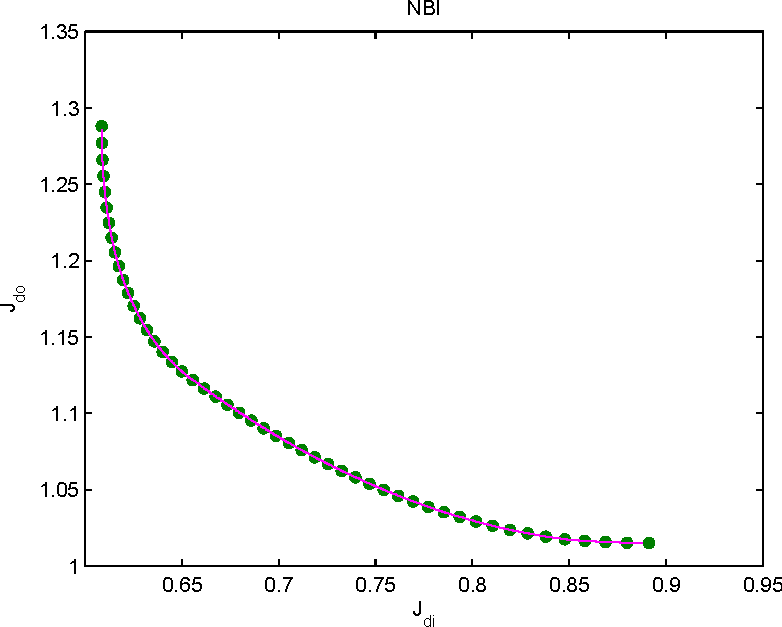
\includegraphics[width=0.8\columnwidth]{ParetoNBIt0_05}%
\caption{Pareto front obtained with NBI method and $\tau_0=0.5$.}%
\label{fig:ParetoNBIt0_05}%
\end{figure}
%

Finally, when the Pareto front is found using the \gls{nnc} method, the points computed are very similar to the ones found with the \gls{nbi} scalarization. The \gls{nnc} case is presented in Fig.~\ref{fig:ParetoNNCt0_05}. 
%
\begin{figure}[tb]%
	\centering
	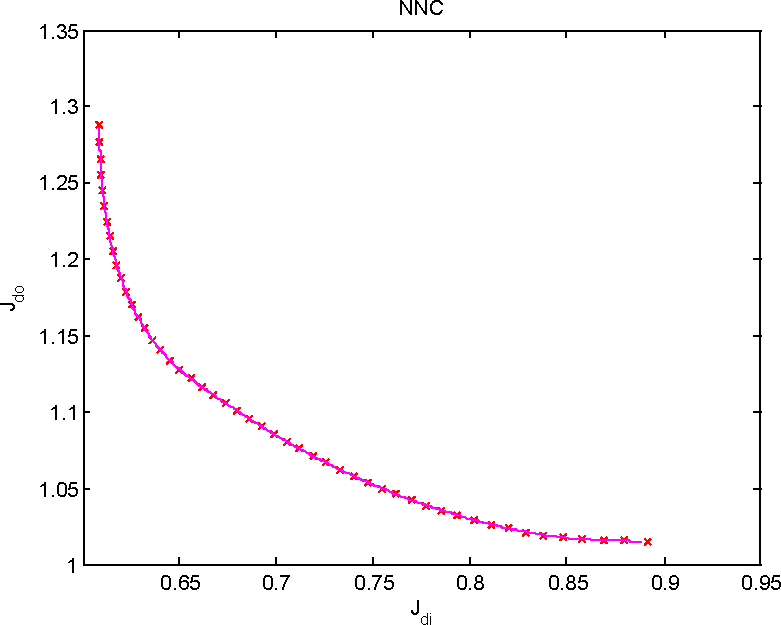
\includegraphics[width=0.8\columnwidth]{ParetoNNCt0_05}%
	\caption{Pareto front obtained with NNC method and $\tau_0=0.5$.}%
	\label{fig:ParetoNNCt0_05}%
\end{figure}
%
Comparing Figure~\ref{fig:ParetoWSt0_05} with Figures~\ref{fig:ParetoNBIt0_05} and \ref{fig:ParetoNNCt0_05}, it is clear that both the \gls{nbi} and \gls{nnc} both are able to find a more accurate approximation of the Pareto front than \gls{ws}. Of course, all the methods are able to find Pareto optimal points, but in order to have a good understanding of the problem, it is important to have a set of point that are representative of the actual behavior of the front. It also is important to note that, the if the actual Pareto front is convex, the results with the \gls{nbi} and \gls{nnc} should be the same. In case of non-convexity, it is possible that the two methods yield to different points in the non-dominated points that should be filtered, following the \gls{nnc} method \cite{Messac2003}.

In Fig.\ref{fig:KpvsAlpha_t0_05.pdf} the comparison between the results for $\kappa_p$ are presented while the values for $\tau_i$ are shown in Fig.~\ref{fig:TivsAlphat0_05}. 
%
\begin{figure}[tb]
\centering
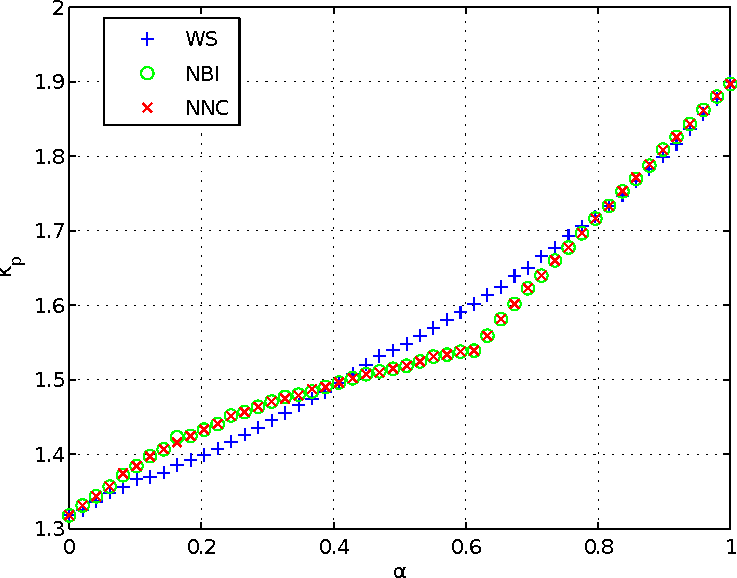
\includegraphics[width=0.8\columnwidth]{KpvsAlpha_t0_05}
\caption{$\kappa_p$ values for all the methods wrt $\alpha$ and with $\tau_0=0.5$.}
\label{fig:KpvsAlpha_t0_05.pdf}
\end{figure}
%%
\begin{figure}[tb]
\centering
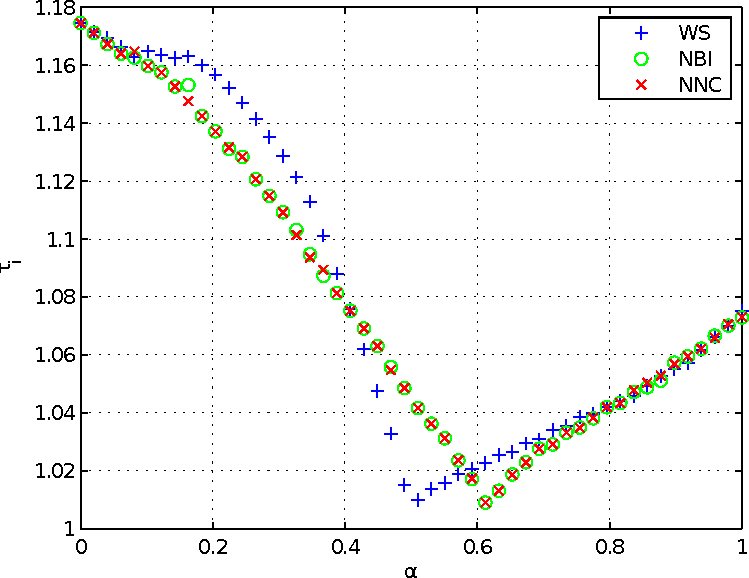
\includegraphics[width=0.8\columnwidth]{TivsAlphat0_05}
\caption{$\tau_i$ values for all the methods wrt $\alpha$ and with $\tau_0=0.5$.}
\label{fig:TivsAlphat0_05}
\end{figure}
%
As it can be seen, \gls{nbi} and \gls{nnc} obtain the exact same points in the Pareto for all values of $\alpha$. However, there are certain differences in the results for $\tau_i$. Since \gls{nbi} depends on a equality constraint, it is more difficult for the optimization algorithm\footnote{For all the methods, the optimization problem was solved using an active-set strategy with a maximum of 1000 iterations and 1000 function evaluations.} to converge to the solution. In fact, for some cases, using the \gls{nbi} methodology leads to more than a thousand function evaluations. Since the maximum was set to one thousand evaluations, for some point the results do not exactly match. However, it is interesting to note that for all three cases, the variation in the values of $\kappa_p$ and $\tau_i$ follows certain pattern. 

The computational performance of the methods has also been considered. Using MATLAB in a PC running Linux with a 3.2.0.2-amd64 kernel and an Intel Core i7 at $1.60$GHz, the results are given in Table~\ref{tab:Results}.
%
\begin{table}[tb]%[ht!]
	\caption{Performance comparison for different optimization methods}
	\centering
	\begin{tabular}{ccccccc}
		\toprule
		\multirow{2}{*}{Method} & \multicolumn{2}{c}{Iterations} & \multicolumn{2}{c}{\begin{tabular}{c} Function\\evaluations\end{tabular}} & \multicolumn{2}{c}{\begin{tabular}{c} Computation\\time (s) \end{tabular}}\\
		\cline{2-7}
		& Average & Max & Average & Max & Average & Max \\
		\hline
		WS & $68.82$ & $109$ & $132.34$ & $212$ & $39.11$ & $63.77$\\
		NBI & $30.78$	& $225$ & $142.86$ & $1003$	& $44.88$	& $320.81$\\
		NNC & $41.28$ &	$297$ & $147.02$ & $1002$ & $71.21$	& $486.47$\\
		%LRC	& $12.24$ &	$34$ & $58.56$ & $136$ & $28.45$ & $66.094$\\
		\bottomrule
	\end{tabular}
	\label{tab:Results}
\end{table}
%
Each Pareto front corresponds to 50 points for $\tau_0=0.5$ and the table gives the values obtained regarding computational performance: number of iterations, number of function evaluations and the time spend during the process. Interestingly, it was found that \gls{nbi} has better performance than \gls{nnc} for this particular case. However, during the computation it was noticed that the \gls{nbi} reached the maximum number of evaluations in four of the fifty points whereas the \gls{nnc} method reach the same limit for just one point. If the results of the \gls{ws} is taken as the base reference, it was found that \gls{nbi} and \gls{nnc} required a lower number of iterations on average, however, they needed more function evaluation ($8\%$ and $11\%$, respectively) and more computation time ($14.74\%$ and $82.05\%$, respectively).

Regarding the computation of all points of the Pareto, it was found that using the \gls{ws} method $32.6$ minutes where needed, using the \gls{nbi} $37.4$ minutes where spend while using the \gls{nnc} method took $59.33$ minutes. However, it is clear that performing the computation of the Pareto front is a computational expensive task, that may no be suitable for an ``online'' tuning procedure. However, it is interesting to consider the case where the front is computed ``offline'' for a family of plants (using the normalized version) and then, use the data directly for the decision making process of choosing the final tuning of the controller.

In the following, the results are analyzed from a control theory point of view and compared with other methodologies.
%------------------------------------------------------------------------
\subsection{Analysis of the results from the control theory perspective}
\label{sec:Control}
%
When the plant is varied from $\tau_0=0.1$ to $\tau_0=2$ in steps of $0.1$, the corresponding Pareto fronts are plotted in Fig.~\ref{fig:Paretos_t0_all}. It was expected that for increasing values $\tau_0$, the values of $J_{di}$ and $J_{do}$ also increase because of the inherent delay of the plant which directly affects the \gls{iae}, the achievable performance.
%
\begin{figure}[tb]%
\centering
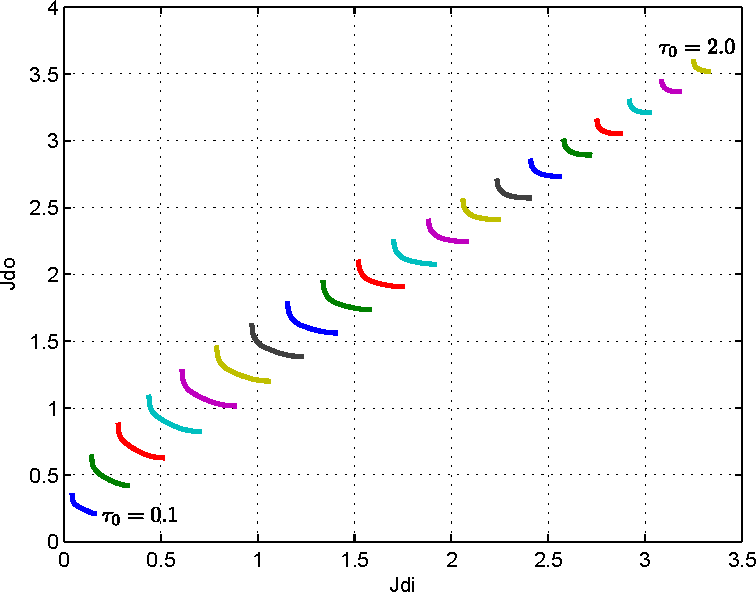
\includegraphics[width=0.8\columnwidth]{Paretos_t0_all}%
\caption{Fifty point Pareto fronts varying $\tau_0$.}%
\label{fig:Paretos_t0_all}%
\end{figure}
%

As it can be seen, depending on $\tau_0$, the values that the cost functions have can be very different. For this reason it may be interesting to compared the Paretos with a normalized version of the cost functions for the same variation on $\tau_0$. This study is presented in Figure~\ref{fig:Paretos_t0_Norm}. %
%
\begin{figure}[tb]%
	\centering
	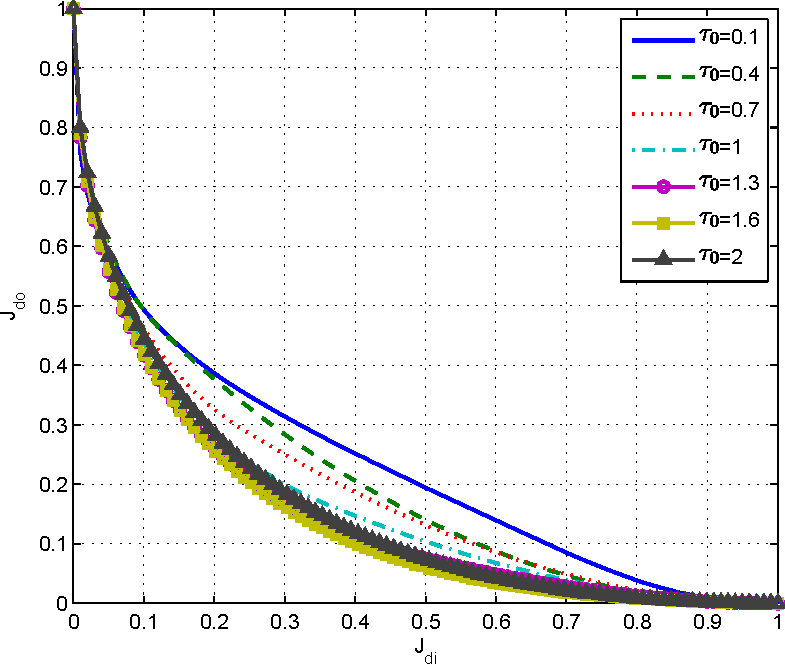
\includegraphics[width=0.8\columnwidth]{Paretos_t0_Norm}%
	\caption{Normalised version of the Pareto front for different values of $\tau_0$.}%
	\label{fig:Paretos_t0_Norm}%
\end{figure}
%
In this figure, all the Paretos have been scaled in order to have its cost functions between 0 and 1. The value 0 represents the lowest value of the cost function while the 1 represents the highest value. Therefore, it can be seen as a degradation value: a value of one represents a total degradation of one of the function (but, preserving the fact that it is Pareto optimal).

It is interesting to note that, if a degradation of around $10\%$ in the input disturbance cost function is allowed, it yields to an improvement of up to $50\%$ in the servo response for all values of $\tau_0$. However, it is interesting to note that, in the other case where the system is initially set to be optimal for servo response (a value of $J_{do} = 0$) if a $10\%$ of degradation is allowed, an improvement between 30\% and 60\% is achieved depending of the value of $\tau_0$. These results show that, by analyzing the Pareto front, an important improvement can be achieved if one of the functions is allowed to be degraded  by just a small amount. But of course, the decision on how much to degrade is entirely up to the decision maker. But it is clear that the Pareto is a good tool to support that decision.

Is it possible to identify a single point in the Pareto front that gives the best compromise between these objectives? Although how much degradation is allowed is a subjective decision of the designer, it may be possible to give an alternative. The point that may be a good start is the point in the Pareto front that is closer to the utopia point. This point can be obtained by minimizing for example:
%
\begin{equation}
\min_{\hat{\theta}}{\; \sqrt{\left( \hat{J}_{di}(\hat{\theta})\right) ^2+\left( \hat{J}_{do}(\hat{\theta})\right)^2}},
\label{eq:Compr}
\end{equation}
%
which represent the Cartesian distance between the Pareto front and the Utopia point

The result for $\tau_0=0.5$ is presented in Fig.~\ref{fig:ComprPoint_t0_05}. It is necessary to use the normalized cost functions in order to give the same importance to both objective functions. 
%
\begin{figure}[tb]
\centering
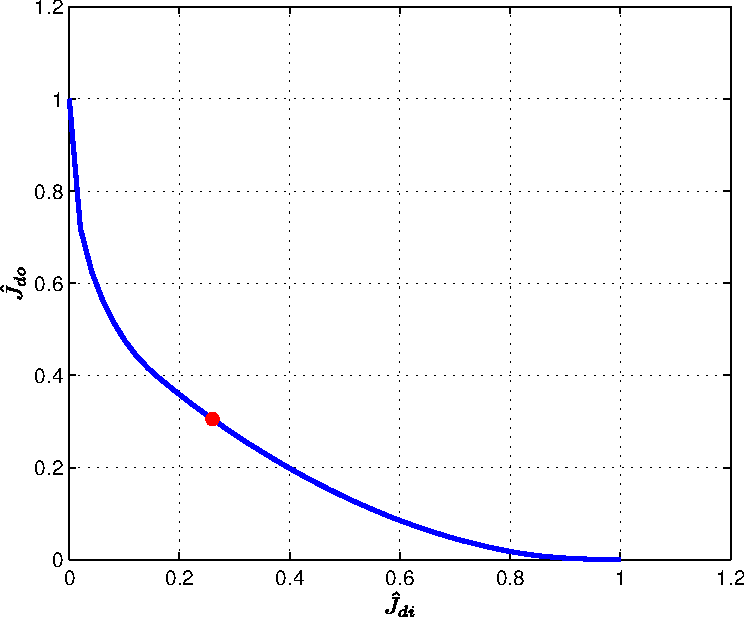
\includegraphics[width=0.8\columnwidth]{ComprPoint_t0_05}
\caption{Best compromise in the Pareto front as given by the Cartesian distance.}
\label{fig:ComprPoint_t0_05}
\end{figure}
%%
As it can be seen, the tuning of the parameters that are closer to the utopia point is the one that produces a degradation of $26\%$ in $\hat{J}_{di}(\hat{\theta})$ and a corresponding $30.52\%$ degradation in $\hat{J}_{do}(\hat{\theta})$. This point may not be suitable for the requirements of the problem at hand, but is a good starting point from where the designer can choose the ``best'' (not necessarily the optimal) solution for the particular problem.

In Figures~\ref{fig:KpvsAlpha} and \ref{fig:TivsAlpha} the variation of the parameters $\kappa_p$ and $\tau_i$ with respect to $\alpha$ for different values of $\tau_0$ are presented. For example, in the case of $\kappa_p$ higher values of $\tau_0$ gives lower values for this parameter. The variation is small with respect to the increase in the degradation of $J_{di}$ (which is represented by $\alpha$ in the figures), except for lower values of $\tau_0$. Something similar happens when $\tau_i$ is analyzed, however, in this case the value of $\tau_i$ increases when $\tau_0$ is larger, but again the variation with respect to the degradation is not very large. This is important to note, because, if the controller does not allow a precise input of the parameter tuning, it may be possible that the desired point in the Pareto front cannot be achieved for some values of $\tau_0$, since small changes in the tuning produce important changes in the degradation (in percentage). However, it has to be noted in Figure~\ref{fig:Paretos_t0_all} that the possible change in \gls{iae} for both input and output disturbances rejection is smaller for higher values of $\tau_0$ than for lower values. The relationship between $\kappa_p$ and $\tau_i$ is presented in Figure~\ref{fig:TivsKp}. The possible range of values is also smaller for higher values of $\tau_0$. 
%
\begin{figure}%
\centering
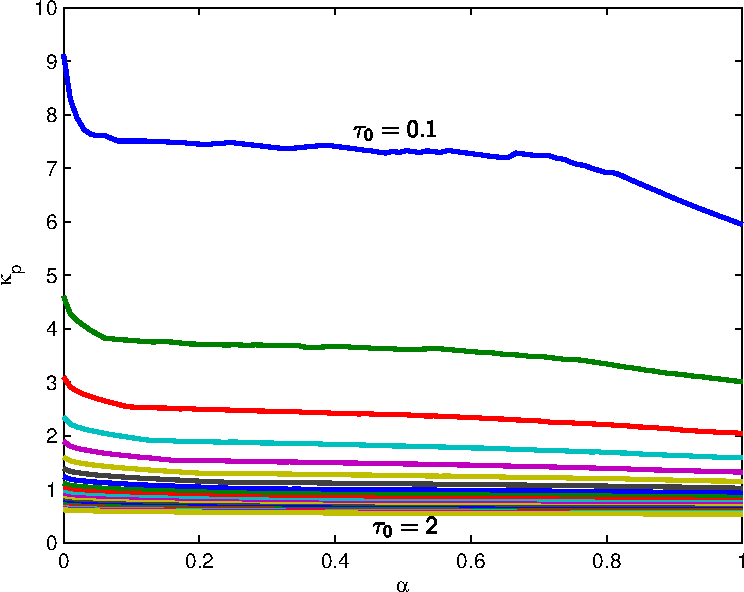
\includegraphics[width=0.8\columnwidth]{KpvsAlpha}%
\caption{Variation of $\kappa_p$ wrt the degradation of the $J_{di}$ cost function ($\alpha$) and $\tau_0=0.5$.}%
\label{fig:KpvsAlpha}%
\end{figure}
%
\begin{figure}%
\centering
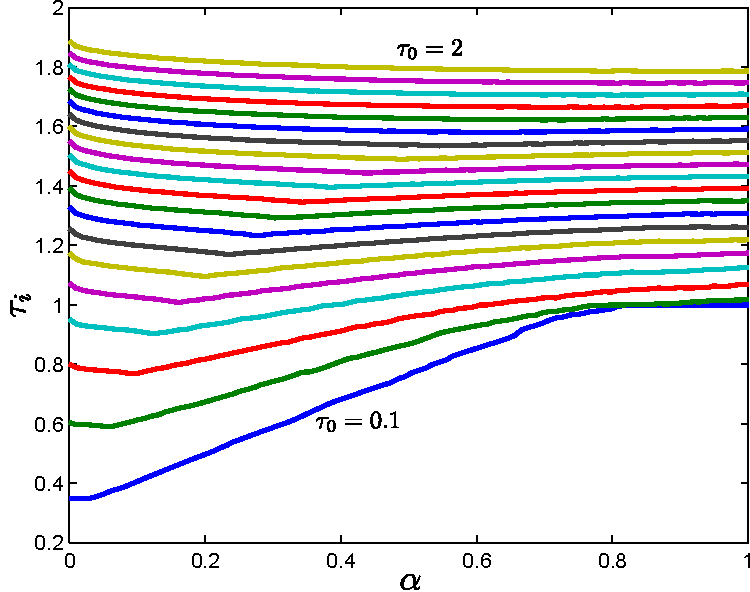
\includegraphics[width=0.8\columnwidth]{TivsAlpha}%
\caption{Variation of $\tau_i$ wrt the degradation of the $J_{di}$ cost function ($\alpha$) and $\tau_0=0.5$.}%
\label{fig:TivsAlpha}%
\end{figure}
%
\begin{figure}%
\centering
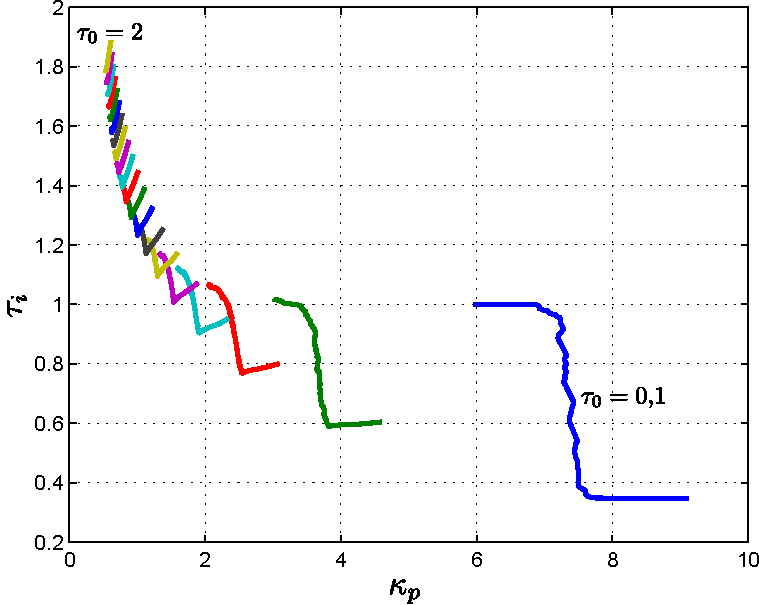
\includegraphics[width=\columnwidth]{TivsKp}%
\caption{$\tau_i$ vs $\kappa_p$ for different values of $\tau_0$.}%
\label{fig:TivsKp}%
\end{figure}
%

It is important to remember that each point of the Pareto front represent a different tuning of a \gls{pi} controller. Therefore it is possible to compare the relationship between more classical ways to tune the controller with the front itself. The controller was tuned using the rules in \citet{ODwyer2000,Astrom1995,Murril1967,Rovira1969,Grimholt2012, Smith1985, Ziegler1942}. Each tuning also can be represented by a point along with the Pareto. This plot is shown in Figure~\ref{fig:PIMethods}. %
%
\begin{figure}%
	\centering
	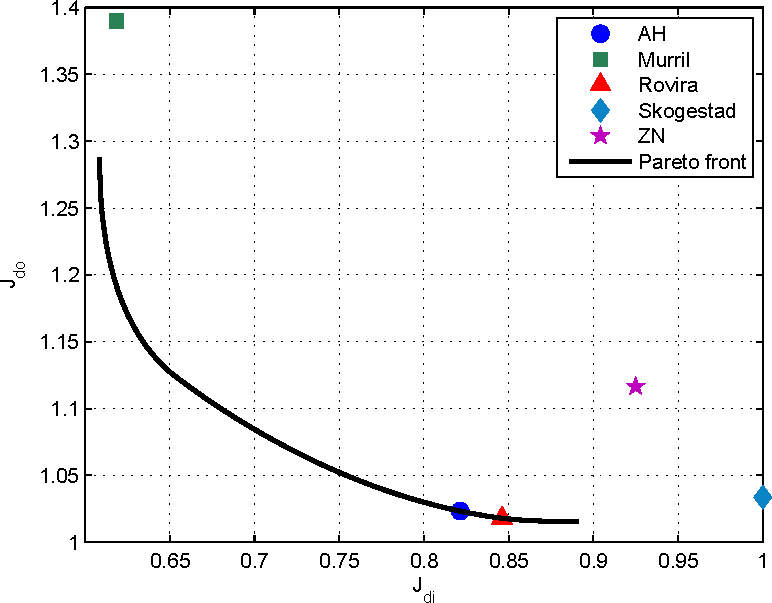
\includegraphics[width=0.8\columnwidth]{PIMethods}%
	\caption{Comparison of several tuning methods within the Pareto front for $\tau_0=0.5$.}%
	\label{fig:PIMethods}%
\end{figure}
%
It is important to note that those methods are not necessarily the result of an optimization problem and therefore, they may not belong to the Pareto.

The tuning of \citet{Murril1967} was created with the intention of minimize the \gls{iae} for input disturbances. This explains the fact that the value of $J_{di}$ for this controller is very close to the anchor point where $J_{di}$ is minimal. In the case of Rovira~\citep{Rovira1969}, it was designed to minimize the servo response of the closed loop controller. In this particular case, given that the controller used in the Pareto is a one degree of freedom \gls{pi}.

In this particular case, minimizing the servo response is exactly the same as minimizing the output disturbance rejection ($J_{do}$) for a two degrees of freedom controller. This is the reason why its tuning point is located at the right hand side of the Pareto front. It was interesting to found out that the tuning in \cite{Astrom1995} (AH in the figure), yield in the Pareto Front, and therefore can be considered also as Pareto optimal. The case of \citet{Grimholt2012} is also interesting because it is almost optimal in the $J_{do}$ sense, but due to its consideration of robustness, its far from the Pareto front given in this particular case. As expected, the method by Ziegler and Nichols \citep{Ziegler1942} (ZN in the figure) is far from optimal, but it is included in this analysis for comparison purposes only.

In this particular section, the obtained Paretos did not considered the robustness of the controlled system. If the \gls{ms} is computed as a function of the degradation of $J_{di}$, the result is a shown in \ref{fig:MsAlpha}.
%
\begin{figure}%
	\centering
	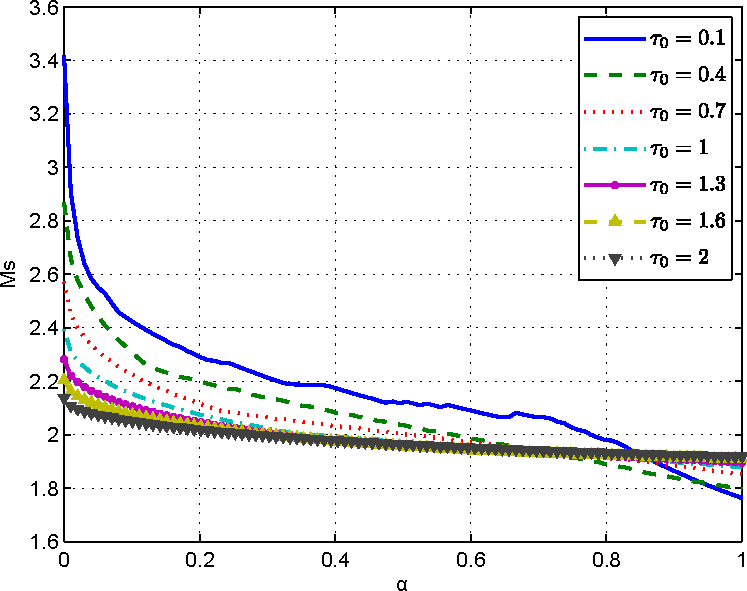
\includegraphics[width=0.8\columnwidth]{MsAlpha}% %\porcentajefig
	\caption{Sensitivity function wrt $\alpha$, varying $\tau_0$.}%
	\label{fig:MsAlpha}%
\end{figure}
%

Of course, the robustness of the controlled system is not good for a real application of the controller. It is generally accepted that a value of two or lower is a desirable, and in this cases, almost all of them has a value of $M_S$ greater than 2. However, it is possible to consider the robustness inside the optimization problem, either as a cost function or as constraint. As an example, consider the case of $\tau_0=0.5$ presented in Figure~\ref{fig:Pareto10000MS16}. When the case for $M_S\leq 1.6$ is considered, the feasible region is shrinks considerably. In this case, the Pareto front for the optimal tuning is outside the new feasible region and therefore, a completely different Pareto front would be obtained when the optimization methods are run with this new constraint.

Depending on the desired value of $M_S$ and the given value of $\tau_0$, it may be possible that the optimal frontier also do satisfy the robustness constraint.
%
\begin{figure}%
\centering
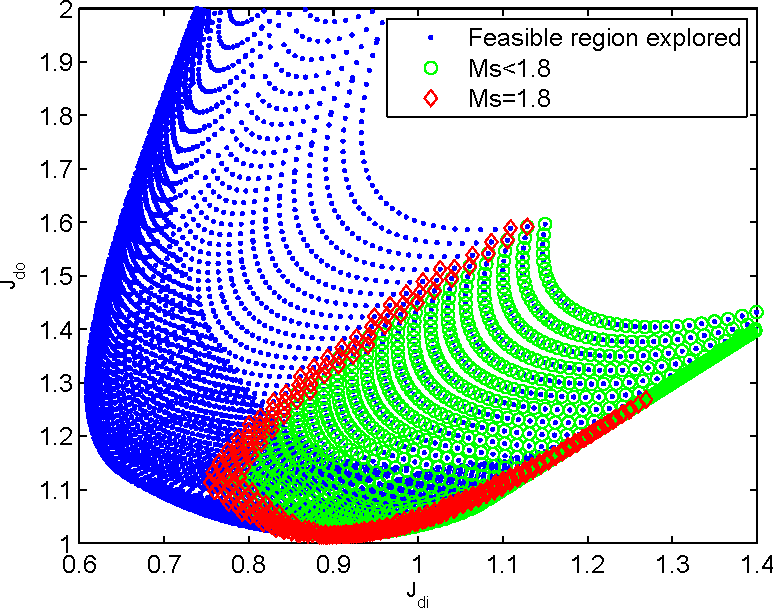
\includegraphics[width=\columnwidth]{Pareto10000MS16}%
\caption{Complete feasible region for $\tau_0=0.5$ and the subregion where $M_S \leq 1.8$.}%
\label{fig:Pareto10000MS16}%
\end{figure}
%
Therefore, since the robustness can be considered just as a constraint in the optimization problem, a tuning methodology that considers both multi-objective optimality and robustness can be obtained using the Pareto front framework and will be the choice in the rest of this book.
%
%---------------------------------------------------------------------------------------
%---------------------------------------------------------------------------------------
%
\section{High-Order Benchmark Plant}
\label{sec:Bechmark}
First the \gls{ennc} method is going to be tested in high order benchmark plant \citep{Astroem2000}. The model of the plant is given by a fourth order transfer function:
\begin{equation}
P(s) = \frac{1}{\prod_{n=0}^{n=3}(0.5^n s+1)}.
\label{eq:benchmarkTF}
\end{equation}

The first step is to obtain a low order model that is able to reflect the main dynamics of the plant. In general, the tuning of \gls{pid} controllers starts with a first or second order model \citep{Alfaro2006}. In this particular case, using a step change as the input signal, the low order model that can be found from this experiment is given by:
%
\begin{equation}
F(s)=\frac{e^{-0.297s}}{(0.9477s+1)(0.6346s+1)},
\label{eq:BenchTFfit}
\end{equation}
%
alternatively, if it is supposed that the ``real'' model of the plant is known, an order reduction procedure, for example, the half-rule method may be used \citep{Skogestad2003}. The comparison between the high order model and the reduced order model in the time domain is presented in %
\begin{figure}[tb]
	\centering
	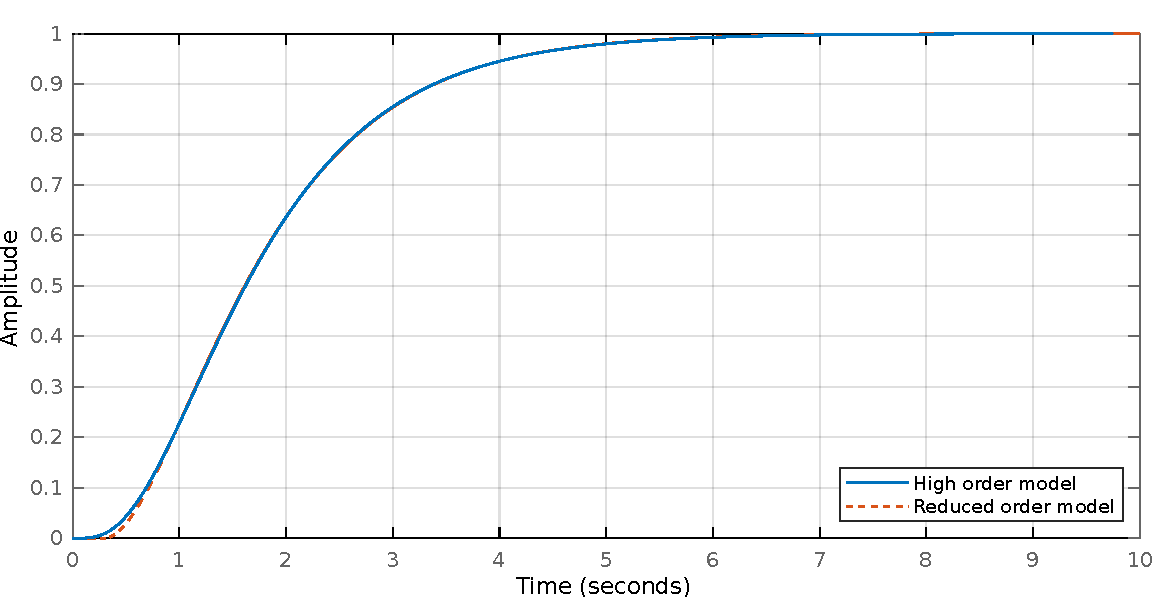
\includegraphics[width=0.9\columnwidth]{Ch7CompRespBench}
	\caption{Comparison between the high and reduced order models.}
	\label{fig:Ch7CompRespBench}
\end{figure}
%
Figure~\ref{fig:Ch7CompRespBench}. As it can be seen, the model represents accurately the dynamics of the original plant and therefore it is considered to be a good approximation of the original model.

The next step is to find the Pareto front for this particular plant. The followed methodology was as presented in Chapter~\ref{chap:PIDMOOP}. For this particular case, only $J_{di}$ and $J_r$ where considered as the cost functions with a \gls{2dof} \gls{pid} controller. In Figure~\ref{fig:paretomodelo}, the obtained Pareto front is presented. 
%^
\begin{figure}[tb]%
	\centering
	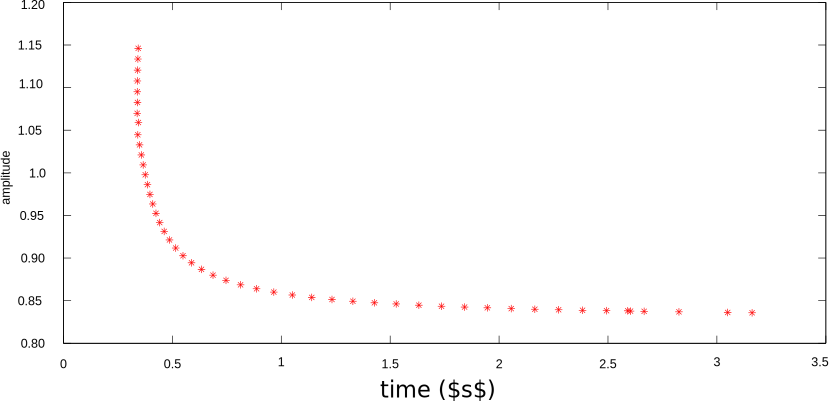
\includegraphics[width=0.9\columnwidth]{paretomodelo}%
	\caption{The Pareto front for the benchmark process.}%
	\label{fig:paretomodelo}%
\end{figure}

The curve has a typical form, with a higher slope for low values of $J_{di}$ and an almost flat slope for higher values. This shape has a particular physical meaning: to improve the response of the $J_{di}$ cost function, the $J_{r}$ value has to be augmented (worsening the servo response), however the degradation is not as much as the improvement in the $J_{di}$ function. This is a clear example of one of the many advantages of using a multi-objective framework for controller tuning and the main reason why is the chosen framework in this book, it gives the decision taker more tools to select the more appropriate tuning for the controllers.

In order to compare the response of the optimal controllers, the tuning for the anchor points are presented along the resposes of the ART$_2$ method \citep{Vilanova2011} and the uSORT$_2$ method\citep{Alfaro2012a}, in order to compare the performance of the closed loop response. It is important to clarify that these two tuning are just the extreme points of the Pareto front, thanks to the ENNC method and that there is a practically and infinite amount of possible parameter tuning to select. The obtained parameters are listed in %
%
%parámetros del controlador
\begin{table}[tb]
	\caption{PID controller parameters using two degrees of freedom.}
	\centering
	\begin{tabular}{@{}*{5}{c}@{}}
		\toprule
		Tuning              &$K_c$       &$T_i$      &$T_d$     & $\beta$ 	\\
		\midrule              
		optimum $J_{di}$     &$3.3750$   & $1.0812$  &$0.3095$  &$0.5466$   \\
		optimum $J_{r}$      &$3.0572$   & $8.4419$  &$0.3986$  &$1.2329$   \\
		$ART_2$             &$3.3657$   & $1.7636$  &$0.4884$  &$0.2971$   \\
		$uSORT_2$           &$3.1708$   & $0.8997$  &$0.3945$  &$0.4731$   \\	
		%
		\bottomrule				
	\end{tabular}
	\label{tab:parametroscontrolador}
\end{table}
%
Table~\ref{tab:parametroscontrolador} for reference. It is important to note that in all cases, the Maximum Sensibility was set to be around $M_s = 2.0$ to ensure a minimum level of robustness.

In Figure~\ref{fig:Ch7cambioreferencia}, the closed-loop responses of all the four controllers are presented for the case of a step change in the setpoint. it was found that precisely the controller in the anchor point of the Pareto front that give the minimum value of $J_r$ is in fact the one that give the best result of all the controllers. However, it has to be noticed that both ART$_2$ and uSORT methods are intended for regulator response mainly, and theredore, it was not expected to have a lower $J_r$. The obtained values are given in Table~\ref{tab:IAEref} where both the \gls{iae} and \gls{ms} are presented. 

On the other hand, the optimal controllers in the regulator mode are presented in Figure~\ref{fig:cambiodi}. Again, as expected, the controller in the anchor point that has the lowest value of $J_{di}$, is the one with the fastest response. Also, it is clear that the other anchor point (the one with the lowest value of $J_r$) has the worst response for disturbance rejection as it was expected. In table \ref{tab:IAEdi}, the corresponding values of IAE for the curves in Figure~\ref{fig:cambiodi} are presented.

The optimal controller for disturbance rejection is presented in figure \ref{fig:cambiodi}. Again, the tuning given by the ENNC method is the fastest response to reach the desired value. As it can be seen, the ART$_2$ and the uSORT$_{2}$ methods fall between these two optimal responses. However, it does not necessarily means that these methods are optimal because they could be dominated by other controllers that are exactly in the front. Only the tuning found with the ENNC method can be considered to be Pareto optimal using the \gls{iae} as the metric. In Table~\ref{tab:IAEdi}, the IAE values of the responses presented in Figure~\ref{fig:cambiodi} are stated, and again the controller that achieves the lower error value is the one that correspond to the anchor point.
%CAMBIO EN VALOR REFERENCIA
\begin{figure}[tb]%
	\centering
	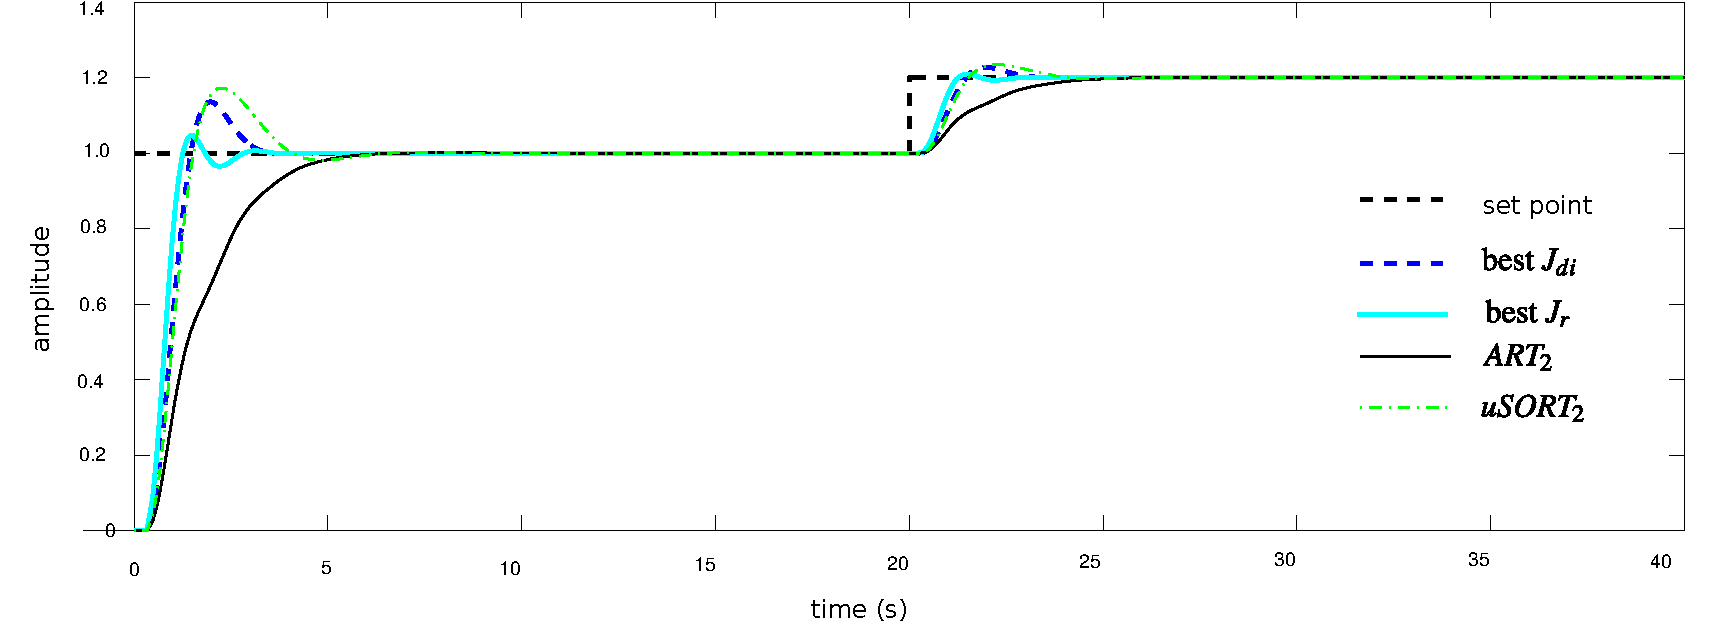
\includegraphics[width=\columnwidth]{Ch7cambioreferencia}%
	\caption{Optimal response of the control system $J_r$}%
	\label{fig:Ch7cambioreferencia}%
\end{figure}
%
%CAMBIO EN PERTURBACIÓN
\begin{figure}[tb]%
	\centering
	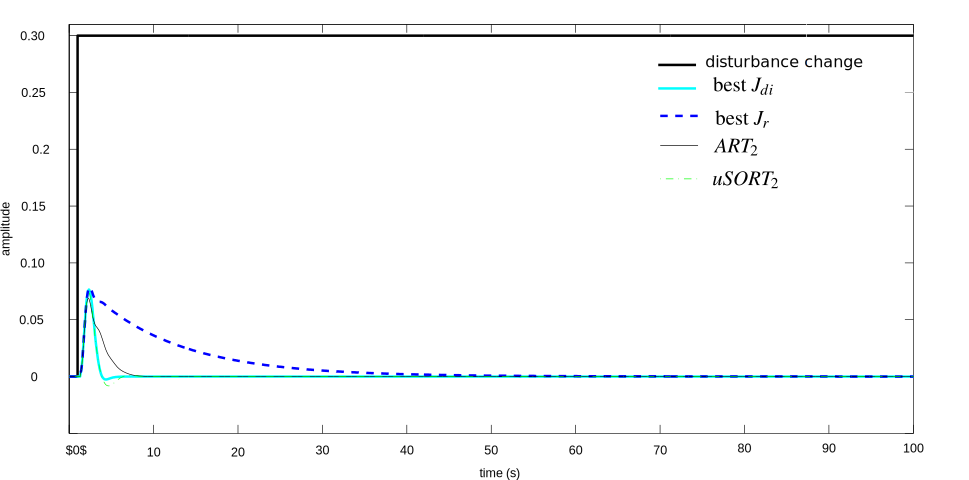
\includegraphics[width=\columnwidth]{cambiodi}%
	\caption{Optimal response of the control system $J_{di}$}%
	\label{fig:cambiodi}%
\end{figure}
%
%IAE ante cambio en valor de referencia
\begin{table}[tb]
	\caption{Servo response for the benchmark system.}
	\centering
	\begin{tabular}{@{}*{3}{c}@{}}
		\toprule
		Tuning             &IAE        &$M_s$   \\
		\midrule              
		optimum $J_{r}$     &$1.004$   & $2$    \\
		optimum $J_{di}$    &$1.297$   & $2$    \\
		$uSORT_2$          &$1.522$   & $2$    \\
		$ART_2$          &$2.121$   & $2$    \\	
		\bottomrule				
	\end{tabular}
	\label{tab:IAEref}
\end{table}
%
%IAE ante cambio en perturbación
\begin{table}[tb]
	\caption{Regulator response for the benchmark system.}
	\centering
	\begin{tabular}{@{}*{3}{c}@{}}
		\toprule
		Tuning            &IAE        &$M_s$   \\
		\midrule              
		optimum $J_{di}$   &$0.1017$   & $2$    \\
		$uSORT_2$          &$0.1095$   & $2$    \\
		$ART_2$            &$0.1574$    & $2$    \\	
		optimum $J_{r}$    &$0.8283$   & $2$    \\
		\bottomrule				
	\end{tabular}
	\label{tab:IAEdi}
\end{table}

It is important to note that in these figures, only two possible points (in fact, the two extreme cases) were considered, but in reality, there are much more options to select for intermediate values of the parameters between these two cases. It has to be noticed that the second order overdamped model is well suited to approximate high order models. Therefore, having done the computation for this particular model as presented in Section~\ref{sec:SolMOOP} allows to tackle almost any real-case of overdamped plants that can be found in the industry.
%-----------------------------------------------------------------------------------------------------------------------------------
\section{LiTaO$_3$ Thin Film Deposition Process}
\label{sec:LiTAO3}
Temperature control is a very important factor in the deposition process of lithium tantalate (LiTaO$_3$) by means of metal organic chemical vapor deposition (MOCVD) \citep{Zhang2004}.

The dynamics of the reactor chamber are characterized by a large lag and time-delay. It is important for the quality of the final product, that the controller follows a predefined temperature profile accurately (servo control) while being able to reject other disturbances (regulatory control).

The model of the MOCVD chamber can be given by:
\begin{equation}
G(s) = \frac{K e^{-L s}}{T s+1},
\label{eq:GsLita}
\end{equation}
%
where the gain $K = 3.2$, the time constant $T = 200$~s and the time-delay $L = 150$~s.

For this case, a two function MOOP is considered with $J_{di}$ and $J_{r}$ as cost functions and a robustness constraint of $M_S = 2.0$. When solving the optimization using the ENNC method, the obtained Pareto front is as given in %
\begin{figure}[tb]
	\centering
	\begin{tikzpicture}
	\begin{axis}[
	xlabel = $J_{di}$,
	ylabel = $J_{r}$,
	grid = major,
	width=0.7\columnwidth,
	xtick={0.7,0.75,...,1.2},
	ytick={1.2,1.22,...,1.5},
	]
	\addplot[mark=none, line width=2pt,] table[x=Jdi, y=Jr]{./tablas/Pareto_LiTa_ms2.dat};
	\end{axis}
	\end{tikzpicture}
	\caption{Pareto front for the LiTaO$_3$ thin film deposition process.}
	\label{fig:LitaPareto}
\end{figure}
%
figure~\ref{fig:LitaPareto}.

Again, the Pareto front let the decision maker to choose between multiple possible solutions. In this particular case, taking the anchor point for minimum value of $J_{di}$ from Figure~\ref{fig:LitaPareto}, it can be seen that, from this point, if $J_{di}$ is degraded by $1.8\%$, it means an improvement of $4.37\%$ for $J_{r}$. This information could only be possible if the Pareto is available is some way, either as a graph or as a set of raw data.

In order to help the control engineer to understand the tuning of the controller, it could be useful to plot the variation of the controller parameters as a function of the degradation of one of the cost functions. Given that the LiTaO$_3$ Thin Film Deposition Process requires to follow a given temperature profile, the control engineer may surely consider $J_r$ as the main function.
%
\begin{figure}[tb]
	\centering
	\subfloat[$K_p$ variation for the LiTaO$_3$ thin film deposition process as a function of $J_r$ degradation.]{
	\begin{tikzpicture}
	\begin{axis}[
	label style={font=\scriptsize},
	tick label style={font=\scriptsize},
	xlabel = $m$ (\%),
	ylabel = $K_p$,
	grid = major,
	width=0.45\columnwidth,
	%scaled x ticks={real:0.01},
	%xtick scale label code/.code={},
	xtick={0,0.2,...,1.2},
	scaled x ticks={real:0.01},
	xtick scale label code/.code={},
	ytick={0.41,0.412,...,0.44},
	y tick label style={
		/pgf/number format/.cd,
		fixed,
		fixed zerofill,
		precision=3,
		/tikz/.cd
	}
	]
	\addplot[mark=none, line width=1pt,color=brown] table[x=Jrn, y=Kp]{./tablas/Pareto_LiTa_ms2.dat};
	\end{axis}
	\end{tikzpicture}
	\label{fig:LitaParetoKp}}\qquad
	%
	\subfloat[$T_i$ variation for the LiTaO$_3$ thin film deposition process as a function of $J_r$ degradation.]{
		\begin{tikzpicture}
		\begin{axis}[
		label style={font=\scriptsize},
		tick label style={font=\scriptsize},
		xlabel = $m$ (\%),
		ylabel = $T_i$,
		grid = major,
		width=0.45\columnwidth,
		xtick={0,0.2,...,1.2},
		scaled x ticks={real:0.01},
		xtick scale label code/.code={},
		%xtick={0,0.1,...,1},
		ytick={200,220,...,320},
		]
		\addplot[mark=none, line width=1pt,color = blue] table[x=Jrn, y=Ti]{./tablas/Pareto_LiTa_ms2.dat};
		\end{axis}
		\end{tikzpicture}
		\label{fig:LitaParetoTi}
		}\\
	%
	\subfloat[$T_d$ variation for the LiTaO$_3$ thin film deposition process as a function of $J_r$ degradation.]{
		\begin{tikzpicture}
		\begin{axis}[
		label style={font=\scriptsize},
		tick label style={font=\scriptsize},
		xlabel = $m$ (\%),
		ylabel = $T_d$,
		grid = major,
		width=0.45\columnwidth,
		xtick={0,0.2,...,1.2},
		scaled x ticks={real:0.01},
		xtick scale label code/.code={},
		%xtick={0,0.1,...,1},
		ytick={40,41,...,55},
		]
		\addplot[mark=none, line width=1pt,color = red] table[x=Jrn, y=Td]{./tablas/Pareto_LiTa_ms2.dat};
		\end{axis}
		\end{tikzpicture}
		\label{fig:LitaParetoTd}
		}\qquad
	%
	\subfloat[$\beta$ variation for the LiTaO$_3$ thin film deposition process as a function of $J_r$ degradation.]{
		\begin{tikzpicture}
		\begin{axis}[
		label style={font=\scriptsize},
		tick label style={font=\scriptsize},
		xlabel = $m$ (\%),
		ylabel = $\beta$,
		grid = major,
		width=0.45\columnwidth,
		xtick={0,0.2,...,1.2},
		scaled x ticks={real:0.01},
		xtick scale label code/.code={},
		%xtick={0,0.1,...,1},
		ytick={0.65,0.7,...,1.05},
		]
		\addplot[mark=none, line width=1pt,color = olive] table[x=Jrn, y=beta]{./tablas/Pareto_LiTa_ms2.dat};
		\end{axis}
		\end{tikzpicture}
		\label{fig:LitaParetoBeta}	
	}
	%
	\caption{Variation of the parameters vs $J_r$ for the  LiTaO$_3$ thin film deposition process.}
	\label{fig:LitaParetoParam}
\end{figure}
%

In Figure~\ref{fig:LitaParetoParam} the values of all the controller parameters are plotted against $m$, where $m$ is defined as the normalized degradation of $J_{r}$ ($m=0$ represents the anchor point where $J_r$ has its lowest value). Looking the behaviour of $K_p$ in Figure~\ref{fig:LitaParetoKp}, it is clear that the value of $K_p$ is kept fairly constant for all values of $m$. This almost negligible variation may be associated to the fact that, for all controller tunings, the maximum sensitivity is set at $M_S = 2$. When this constraint is not taken into account, the value of $K_p$ may have large variations as in the example in Section~\ref{sec:CSTH}.

For the case of the integral time $T_i$, the behavior of this parameter is plotted in Figure~\ref{fig:LitaParetoTi}. Note that, contrary to the case of $K_p$, the variation is highly dependent of $J_r$ and fairly smooth, which is desirable if the interest is to find a tuning rule. However, for the derivative time $T_d$ in Figure~\ref{fig:LitaParetoTd}, it can be seen that the variation is important but the behavior is not as near as smooth as in the case of $T_i$. Finally and the setpoint weight factor $\beta$, also has a piece-wise behavior with respect to $J_r$ and also the variation of its value is important. Nevertheless, once computed the corresponding tunings of all the controllers of the Pareto, the task is just to decide and pick which one is more appropriate for the task.

The response of the controlled system to a setpoint step change is presented in %
%
\begin{figure}[tb]
	\centering
	\begin{tikzpicture}
	\begin{axis}[
	label style={font=\scriptsize},
	tick label style={font=\scriptsize},
	xlabel = time~(s),
	ylabel = output,
	legend cell align=left,
	legend style = {legend pos = south east, font=\scriptsize},%{at={(1,0.05)}, anchor=south east},%
	grid = major,
	width=\columnwidth,
	%scaled x ticks={real:0.01},
	%xtick scale label code/.code={},
	xtick={0,200,...,1600},
	%ytick={41,42,...,52},
	]
	\addplot[mark=none, color=red] table[x=time, y=r]{./tablas/TestServo.dat};
	\addplot[mark=none,dashed, color=blue] table[x=time, y=yservo]{./tablas/TestServo.dat};
	\addplot[mark=none,densely dashdotdotted, color=olive] table[x=time, y=yreg]{./tablas/TestServo.dat};
	\addplot[mark=none,dashdotted, color=magenta] table[x=time, y=yusort]{./tablas/TestServo.dat};
	\legend{Reference,$m=0\%$ (IAE=$244.66$), $m=100\%$ (IAE=$285.64$),uSORT$_2$ (IAE=$304.39$)}
	\end{axis}
	\end{tikzpicture}
	\caption{Servo response of the LiTaO$_3$ thin film deposition process with tree different tuning.}
	\label{fig:LitaServo}
\end{figure}
%
figure~\ref{fig:LitaServo} and for a step signal in the input disturbance in %
%
\begin{figure}[tb]
	\centering
	\begin{tikzpicture}
	\begin{axis}[
	label style={font=\scriptsize},
	tick label style={font=\scriptsize},
	xlabel = time~(s),
	ylabel = output,
	legend cell align=left,
	legend style = {at={(1.05,1)}, anchor=north east, font=\scriptsize},%{legend pos = north east},%
	grid = major,
	width=\columnwidth,
	%scaled x ticks={real:0.01},
	%xtick scale label code/.code={},
	xtick={0,200,...,1600},
	%ytick={41,42,...,52},
	]
	\addplot[mark=none, color=red] table[x=time, y=di]{./tablas/TestReg.dat};
	\addplot[mark=none,dashed, color=blue] table[x=time, y=yservo]{./tablas/TestReg.dat};
	\addplot[mark=none,densely dashdotdotted, color=olive] table[x=time, y=yreg]{./tablas/TestReg.dat};
	\addplot[mark=none,dashdotted, color=magenta] table[x=time, y=yusort]{./tablas/TestReg.dat};
	\legend{Disturbance, $m=0\%$ (IAE=$724.24$), $m=100\%$ (IAE=$502.65$),uSORT$_2$ (IAE=$522.00$)}
	\end{axis}
	\end{tikzpicture}
	\caption{Regulation response of the LiTaO$_3$ thin film deposition process with tree different tuning.}
	\label{fig:LitaReg}
\end{figure}
%
figure~\ref{fig:LitaReg}. For both cases, the anchor points controllers where compared against the uSORT$_2$ tuning rule \citep{Alfaro2012}, since both uses a \gls{2dof} \gls{pid} controller structure and both attempt to minimize an \gls{iae} cost function.

Take into account the response presented in Figure~\ref{fig:LitaServo}. The response of the controlled system is compared against the uSORT$_2$ method as in Section~\ref{sec:Bechmark} given that in this particular example the value of \gls{ms} is also considered. Given that the responses taken from the Pareto are the extreme cases, it is to be expected that all other responses in the Pareto are going to be between these two. Therefore, all the controllers in the Pareto surpass the servo response of the uSORT$_2$, which is not a surprising result given that the uSORT$_2$ method is said to be suboptimal with respect to the servo response, as it is primarily optimized for regulation.

For this same reason, when examining the responses in Figure~\ref{fig:LitaReg} for the disturbance rejection case, it can be seen that the uSORT$_2$ response is close to the case of $m = 100\%$ and this is exactly what it was expected since the uSORT$_2$ method was intended for regulation. Of course, the tuning of the other anchor point has a much worse response, and therefore, the uSORT$_2$ response lies between these two extremes. However, this fact does not mean that the uSORT$_2$ method is optimal in the Pareto sense, because, it may  be possible to find a better servo response with a similar regulation \gls{iae}.

Finally to consciously be aware of the advantage of computing the Pareto front, in %
%
\begin{figure}[tb]
	\centering
	\begin{tikzpicture}
	\begin{axis}[
	label style={font=\scriptsize},
	tick label style={font=\scriptsize},
	xlabel = time~(s),
	ylabel = output,
	legend cell align=left,
	legend style = {legend pos = south east, font=\scriptsize},%{at={(1,0.05)}, anchor=south east},
	grid = major,
	width=\columnwidth,
	%scaled x ticks={real:0.01},
	%xtick scale label code/.code={},
	xtick={0,200,...,1600},
	%ytick={41,42,...,52},
	]
	\addplot[mark=none, color=red] table[x=time, y=y1.00]{./tablas/TestParetoServo.dat};
	\addplot[mark=none,dashed, color=blue] table[x=time, y=y0.61]{./tablas/TestParetoServo.dat};
	\addplot[mark=none,densely dashdotdotted, color=olive] table[x=time, y=y0.31]{./tablas/TestParetoServo.dat};
	\addplot[mark=none,dotted, color=magenta] table[x=time, y=y0.12]{./tablas/TestParetoServo.dat};
	\addplot[mark=none,dashdotted, color=cyan] table[x=time, y=y0.00]{./tablas/TestParetoServo.dat};
	\legend{$m=100\%$, $m=61\%$,$m=31\%$,$m=12\%$,$m=0\%$}
	\end{axis}
	\end{tikzpicture}
	\caption{Servo response of the LiTaO$_3$ thin film deposition process varying the tuning across the Pareto front with different degradations.}
	\label{fig:LitaServoParetoResp}
\end{figure}
%
figure~\ref{fig:LitaServoParetoResp}, five points of the Pareto front where selected ranging from $m=100\%$ to $m=0\%$ and the reference tracking response was plot in the same axis. As before, the front was found with the constraint $M_{S,max}\leq 2.0$. The fact that, among all possible controllers computed, at the end only one of them is going to be selected, may  be seen as a ``waste'' of resources. And this surely may be true if the Pareto is computed for every single case. However, if a general case is computed beforehand and a tool is used to select one of the many controllers, the Pareto front then can be seen more advantageous and certainly more useful for the decision maker. An example of such case is presented in Section~\ref{sec:PIDCSTH}. 

\bibliographystyle{spbasic}
\bibliography{ReferenciasMulti}
\chapter{PID tuning as a multi-objective optimization method}
\label{chap:PIDMOOP}

%-----------------------------
\section{Solution of the multi-objective optimization tuning}
\label{sec:SolMOOP}
When solving the \gls{moop} presented in \eqref{eq:probmoo} for different normalized plants, one is able to find a family of Pareto fronts. The script used to find these fronts can be found in the companion software for this book\footnote{\textbf{PONER EL NOMBRE DEL SCRIPT}}.

Defining the normalized variable $\hat{s}=T s$, the time delay for the normalized plant, $\tau_0$, becomes:
\begin{equation}
\tau_0 = \frac{L}{T},
\label{eq:tauNorm}
\end{equation}
%

Then, one is able to find the corresponding Pareto front for the normalized plant, that represents many combinations of lag time and dead time.
%

The Pareto front was found for each normalized plant with approximately 1000 points for each front. Notices that each of these points represents a different tuning (and since the optimization was done for \gls{2dof} controllers, each point has a different value for $\kappa_p$, $\tau_i$, $\tau_d$ and $\beta$), the total possible Pareto optimal \gls{pid} controllers found, reaches approximately 100 000 different controllers for all the totality of the plants. All these controller tunings, can also be found in the companion software of this book as comma separated values.

\section{Viability for tuning rules}
\label{sec:TuningRulesMOOP}
In this section, an example of how to use the gathered data from the Pareto front is presented in order to find a tuning rule. The results that are presented here where first documented in \cite{Moya2017}.

For this particular example, the variable $a$ takes values from $0$ to $1$ in $0.1$ steps and $\tau_0$ takes values from $1$ to $2$ in $0.1$ steps and $M_{s,max}=2$. However, the complete set of data also has values for $\tau_0 < 1$.

The methodology after finding the data is to perform a curve fitting procedure to find equations useful to compute the value of $\kappa_p$, $\tau_i$, $\tau_d$ and $beta$ as a function of $a$ and $\tau_0$ and a factor of degradation of the cost functions.

Notice that the idea is that, knowing the model of the plant, the values of the controller parameters can be computed without needing to perform all the optimization, and also the decision maker can also select the weight for each cost function in order to find a single set of parameters.

This idea of "allowed degradation" is now introduced. Considered that $J_{di}$ and $J_{do}$ are normalized as:
%
\begin{align}
\delta &= \frac{J_{di}(\theta)-J_{di, min}(\theta)}{J_{di,max}(\theta)-J_{di,min}(\theta)},\label{eq:delta}\\
\gamma &= \frac{J_{do}(\theta)-J_{do, min}(\theta)}{J_{do,max}(\theta)-J_{do,min}(\theta)},\label{eq:gamma}
\end{align}
%
where both $0 \le \delta \le 1$ and $0 \le \gamma \le 1$. Then, these variables can be understood as the degradation of the function, considering the minimum value of the cost function as its optimal. Then a value of $\delta=1$ represents a degradation of 100\% of the $J_{di}$ cost function. It is important to notice that the Pareto front is constructed from three different cost functions. Therefore, if one select the value of the allowed degradation for two functions (in this case, $\delta$ and $\gamma$), the logical step is to choose the lowest value of $J_r$ that complies with the maximum degradation of the other two functions. Then for example,  if $\delta=\gamma=1$, which means that the decision maker is willing to allowed a complete degradation of $J_{di}$ and $J_{do}$, the resulting tuning is expected to represent the optimal tuning for servo control.

Now, it is important to understand that the ``degraded'' tuning, is also optimal in the Pareto sense, because all found tunings are optimal. Therefore, in these frame, a degraded tuning does not mean a ``bad'' tuning, it is just the result of a choice decision when selecting the final optimal controller. In all Pareto decisions, a compromise has to be made when selecting the final solution.

The work done to find the tuning rules, summed up to almost two hundred and twenty regressions for all values of $a$ and $\tau_0$ in order to find the complete set of parameters $\bm{\theta}$.

After different heuristic tests, the regression analysis showed that a second order fit gave the best results for $\kappa_p$, $\tau_i$ and $\tau_d$,  while  a first order fit for $\beta$ was enough to model the variation of this parameter. 

The tuning rule for all controller parameters are proposed to be as:  
%
\begin{align}
\kappa_p &= p_{00}+p_{01}\cdot\gamma+p_{02}\cdot\delta\nonumber\\
&\quad + p_{03}\cdot\gamma^2+p_{04}\cdot\gamma\cdot \delta+p_{05}\cdot\delta^2,\label{E:eqkp}\\
%
\tau_i &= p_{10}+p_{11}\cdot\gamma+p_{12}\cdot\delta\nonumber\\
&\quad + p_{13}\cdot\gamma^2+p_{14}\cdot\gamma\cdot \delta+p_{15}\cdot\delta^2,\label{E:eqTi}\\
%
\tau_d &= p_{20}+p_{21}\cdot\gamma+p_{22}\cdot\delta\nonumber\\
&\quad+p_{23}\cdot\gamma^2+p_{24}\cdot\gamma\cdot \delta+p_{25}\cdot\delta^2,\label{E:eqTd}\\
%
\beta &=p_{30}+p_{31}\cdot\gamma+p_{32}\cdot\delta,\label{E:eqbeta}
\end{align}
%

The coefficients $p_{ij}$, where $i=\{0,1,2,3\}$ and $j=\{0,1,2,3,4,5\}$, depend on $a$ and $\tau_0$. The corresponding fits of $\kappa_p$, $\tau_i$, $\tau_d$ and $\beta$, are shown in Fig.~\ref{F:cftoolkp}. \ref{F:cftoolTi}, \ref{F:cftoolTd} and \ref{F:cftoolbeta} for $a=0.1$ and $\tau_{0}=1$.   % a second order surface was found to be the best fit for all eleven fits overall, as shown in figure \ref{F:firstfit}.
%
\begin{figure}[tb]
	\centering
	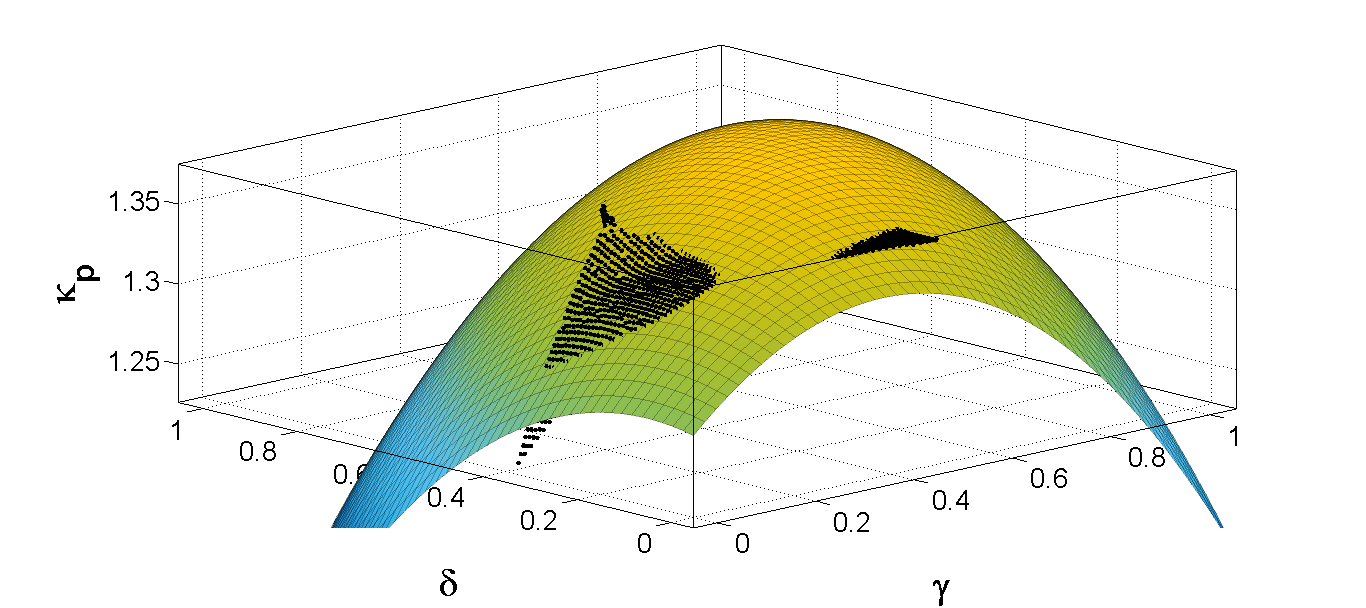
\includegraphics[width=\columnwidth]{kpfit2.png}
	\caption{Second order fit for $\kappa_p$ when $a=0.1$ and $\tau_{0}=1$}
	\label{F:cftoolkp}
\end{figure}
%
\begin{figure}[tb]
	\centering
	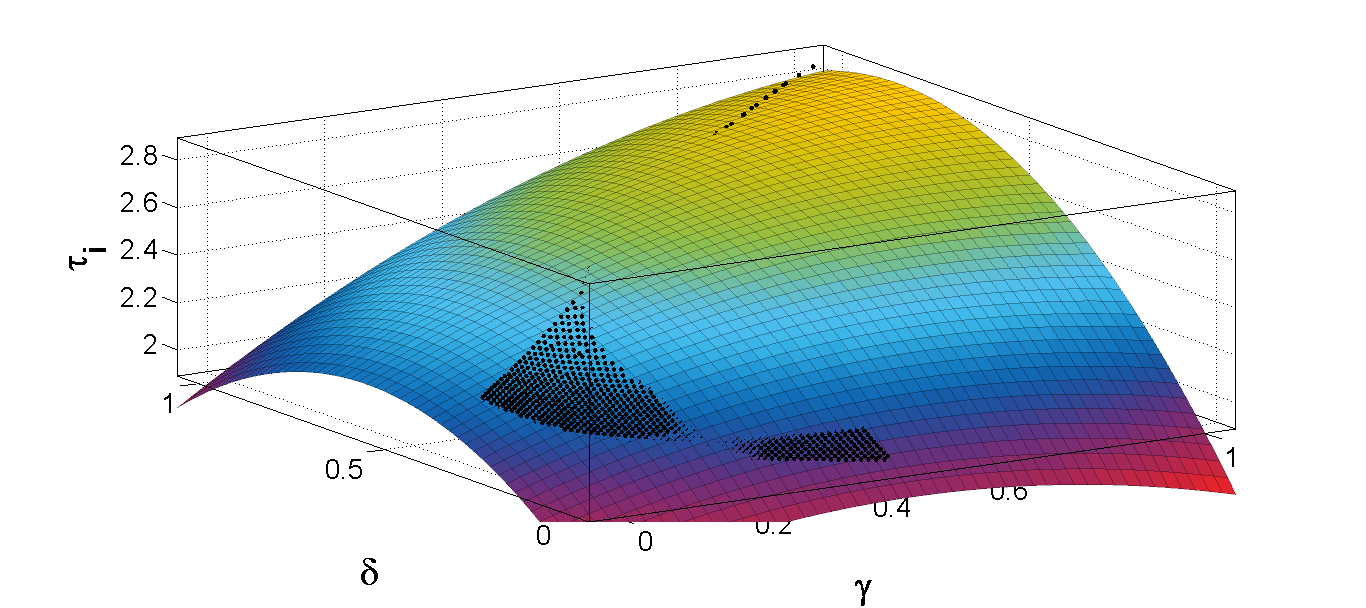
\includegraphics[width=\columnwidth]{Tifit2.png}
	\caption{Second order fit for $\tau_i$ when $a=0.1$ and $\tau_0=1$}
	\label{F:cftoolTi}
\end{figure}
%
\begin{figure}[tb]
	\centering
	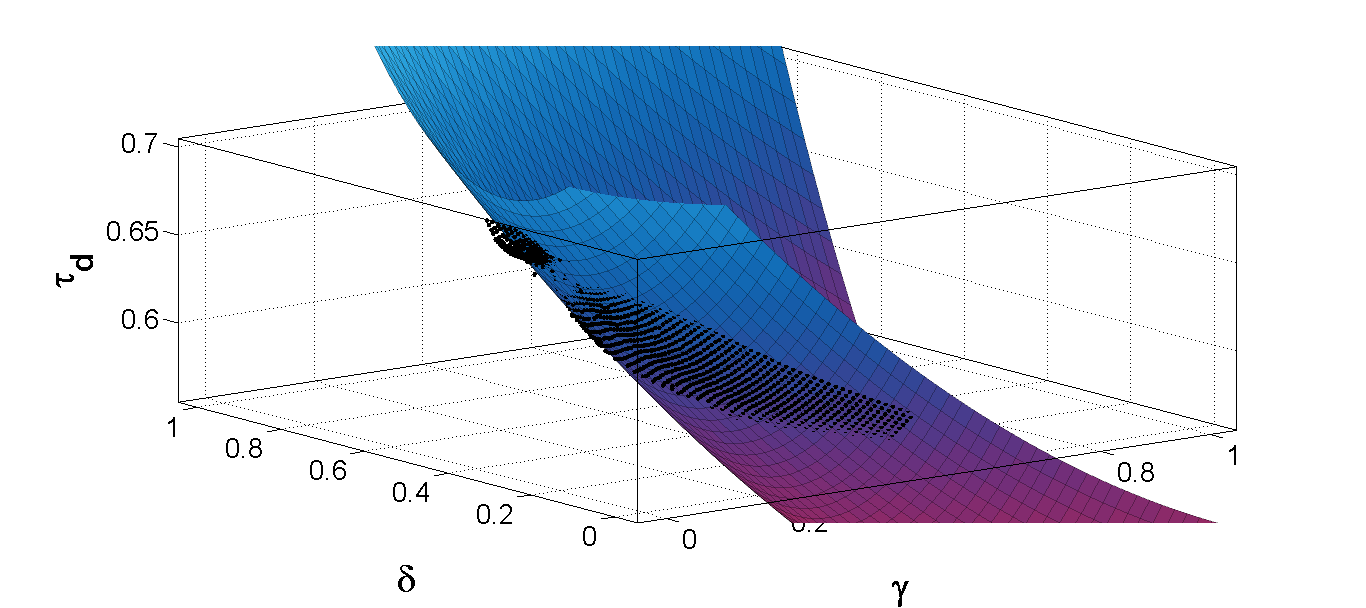
\includegraphics[width=0.5\textwidth]{Tdfit2.png}
	\caption{Second order fit for $\tau_d$ when $a=0.1$ and $\tau_0=1$}
	\label{F:cftoolTd}
\end{figure}
%
\begin{figure}[tb]
	\centering
	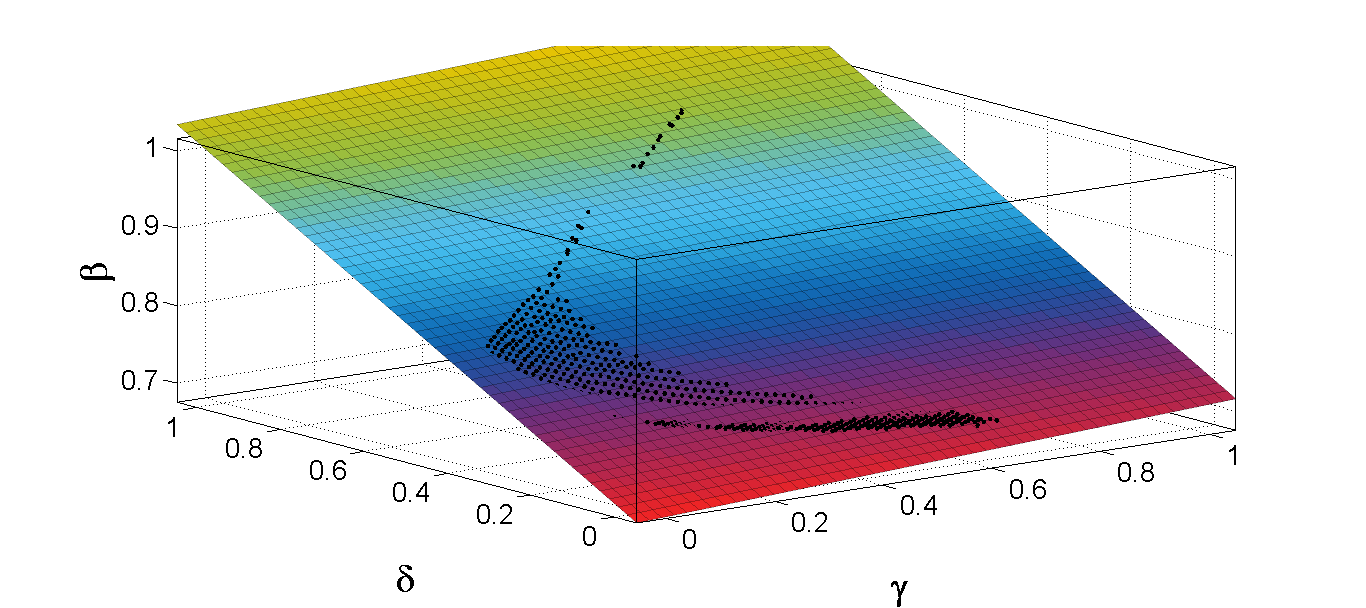
\includegraphics[width=0.5\textwidth]{betafit2.png}
	\caption{First order fit for $\beta$ when $a=0.1$ and $\tau_0=1$}
	\label{F:cftoolbeta}
\end{figure}

It is important to notice an important caveat. In those figures, the values that belong to the computed Pareto are shown as dots, while the corresponding regression is ploted as a 3D surface. It can be noticed that the domain of the regressions is larger than the actual results of the Pareto. Even thought the fitting is good (around $R=0.9$), the regression represents interpolation and extrapolation from the real data. Therefore, it is important too check how well the regression works and to not exceed the limits where it yields good results.

Going back to the $p_{ij}$, it has to be notice that the value of these parameters, depends on the model of the plant. Therefore, it is required to find another set of regressions over these parameters in terms of $a$ and $\tau_0$. Therefore, a curve fitting procedure is also required for each $p_{ij}$. As an example of these regressions, 
%
\begin{figure}[tb]
	\centering
	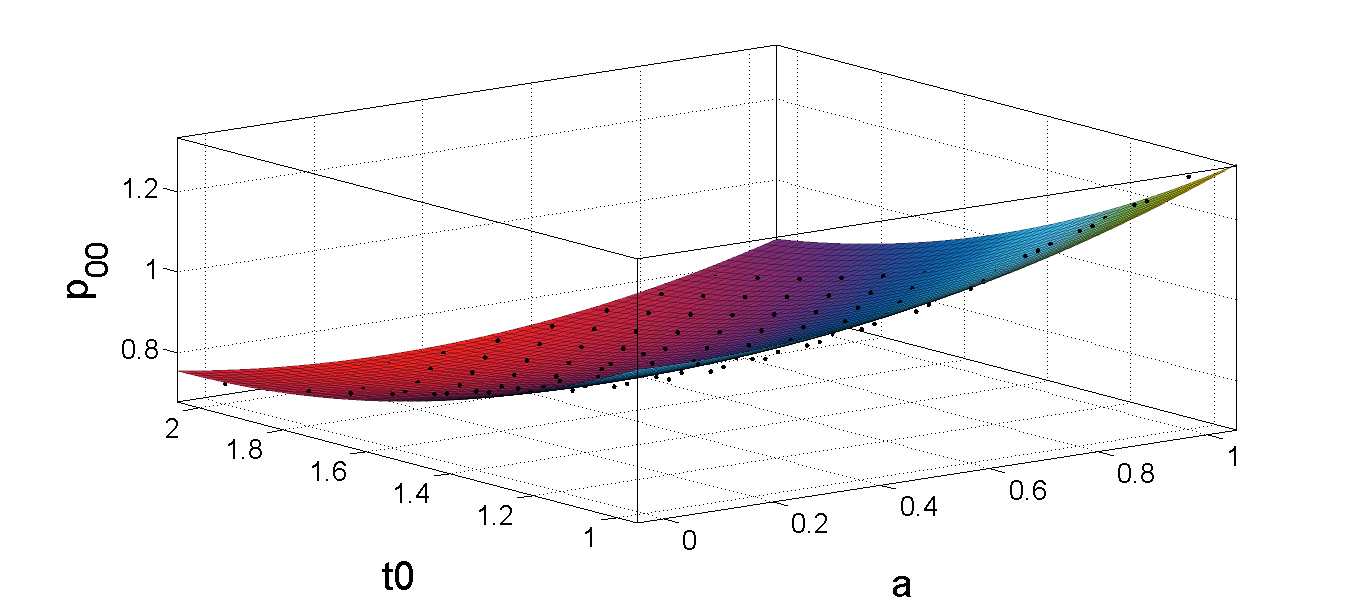
\includegraphics[width=0.5\textwidth]{./a00fit2.png}
	\caption{Second order fit for $p_{00}$ in $\kappa_p$}
	\label{F:coeff}
\end{figure}
%
Fig.~\ref{F:coeff} shows the result for $p_{00}$ parameter as a function of $a$ and $\tau_0$. The selected fit for every coefficient in the range of $1\leq \tau_0 \leq2$, was also a second order polinomial. The equation that is considered has the form:
%
\begin{equation}
p_{ij} = b_{j0}+b_{j1}a+b_{j2} \tau_0+b_{j3}a^2+b_{j4}a \tau_0+b_{j5}\tau_0^2 .
\label{E:coeff}
\end{equation}

Another two hundred and twenty regressions were made for all $p_{ij}$. The results for every coefficient are shown in Table~\ref{T:T1} for $kappa_p$, Table~\ref{T:ti} for the integral time, Table~\ref{T:td} for the derivative time and Table~\ref{T:beta} for $\beta$.

% Please add the following required packages to your document preamble:
% \usepackage{multirow}
%\begin{table}
%\centering
%\caption{Parameters for $\kappa_p$.}
%\label{T:T1}
%\begin{tabular}{|c|l|l|}
%\hline
%\multicolumn{3}{|c|}{$\kappa_p$ coefficients}           \\ \hline
%$p_{ij}$                  & \multicolumn{2}{c|}{$b_{ik}$} \\ \hline
%\multirow{6}{*}{$p_{00}$} & $b_{00}$      & 1.8203        \\ \cline{2-3} 
%                     & $b_{01}$      & 0.12765       \\ \cline{2-3} 
%                     & $b_{02}$      & -1.0484       \\ \cline{2-3} 
%                     & $b_{03}$      & 0.27085       \\ \cline{2-3} 
%                     & $b_{04}$      & -0.15141      \\ \cline{2-3} 
%                     & $b_{05}$      & 0.25505       \\ \hline
%\multirow{6}{*}{$p_{01}$} & $b_{10}$      & 0.32832       \\ \cline{2-3} 
%                     & $b_{11}$      & 0.22439       \\ \cline{2-3} 
%                     & $b_{12}$      & -0.26761      \\ \cline{2-3} 
%                     & $b_{13}$      & -0.022374     \\ \cline{2-3} 
%                     & $b_{14}$      & -0.068708     \\ \cline{2-3} 
%                     & $b_{15}$      & 0.076273      \\ \hline
%\multirow{6}{*}{$p_{02}$} & $b_{20}$      & 0.29122       \\ \cline{2-3} 
%                     & $b_{21}$      & -0.12878      \\ \cline{2-3} 
%                     & $b_{22}$      & -0.25003      \\ \cline{2-3} 
%                     & $b_{23}$      & 0.10461       \\ \cline{2-3} 
%                     & $b_{24}$      & 0.0048329     \\ \cline{2-3} 
%                     & $b_{25}$      & 0.059478      \\ \hline
%\multirow{6}{*}{$p_{03}$} & $b_{30}$      & 0.042733      \\ \cline{2-3} 
%                     & $b_{31}$      & -0.52048      \\ \cline{2-3} 
%                     & $b_{32}$      & -0.25437      \\ \cline{2-3} 
%                     & $b_{33}$      & 0.47345       \\ \cline{2-3} 
%                     & $b_{34}$      & -0.11069      \\ \cline{2-3} 
%                     & $b_{35}$      & 0.078691      \\ \hline
%\multirow{6}{*}{$p_{04}$} & $b_{40}$      & -0.077455     \\ \cline{2-3} 
%                     & $b_{41}$      & 0.61083       \\ \cline{2-3} 
%                     & $b_{42}$      & 0.24951       \\ \cline{2-3} 
%                     & $b_{43}$      & -0.60316      \\ \cline{2-3} 
%                     & $b_{44}$      & 0.19685       \\ \cline{2-3} 
%                     & $b_{45}$      & -0.071314     \\ \hline
%\multirow{6}{*}{$p_{05}$} & $b_{50}$      & -0.41226      \\ \cline{2-3} 
%                     & $b_{51}$      & -0.24733      \\ \cline{2-3} 
%                     & $b_{52}$      & 0.29554       \\ \cline{2-3} 
%                     & $b_{53}$      & 0.080236      \\ \cline{2-3} 
%                     & $b_{54}$      & 0.013411      \\ \cline{2-3} 
%                     & $b_{55}$      & -0.091089     \\ \hline
%\end{tabular}
%\end{table}
%
\begin{table}[tb]
	\centering
	\caption{Coefficients for $\kappa_p$.}
	\label{T:T1}
	\begin{tabular}{@{}cll|cll@{}}
		\hline
		%\multicolumn{6}{c}{$\kappa_p$ coefficients}           \\ \hline
		$p_{ij}$                  & \multicolumn{2}{c}{$b_{ik}$} & $p_{ij}$ & \multicolumn{2}{c}{$b_{ik}$}\\
		\hline
		\multirow{6}{*}{$p_{00}$} & $b_{00}$  & $1.820$ &   \multirow{6}{*}{$p_{01}$} & $b_{10}$ & $0.328$ \\ % \cline{2-3} \cline{5-6}
		& $b_{01}$      & $0.128$   &  	& $b_{11}$      & $0.224$ \\ % \cline{2-3} \cline{5-6}
		& $b_{02}$      & $-1.048$   &	& $b_{12}$      & $-0.268$ \\ % \cline{2-3} \cline{5-6}
		& $b_{03}$      & $0.270$   &	& $b_{13}$      & $-0.022$ \\ % \cline{2-3} \cline{5-6}
		& $b_{04}$      & $-0.151$  & 	& $b_{14}$      & $-0.069$  \\ % \cline{2-3} \cline{5-6}
		& $b_{05}$      & $0.255$   &	& $b_{15}$      & $0.076$    \\ \hline
		%
		\multirow{6}{*}{$p_{02}$} & $b_{20}$  & $0.291$	& \multirow{6}{*}{$p_{03}$} & $b_{30}$ & $0.043$ \\ % \cline{2-3} \cline{5-6}
		& $b_{21}$      & $-0.129$   & & $b_{31}$      & $-0.520$  \\ % \cline{2-3} \cline{5-6}
		& $b_{22}$      & $-0.250$   & & $b_{32}$      & $-0.254$  \\ % \cline{2-3} \cline{5-6}
		& $b_{23}$      & $0.105$    & & $b_{33}$      & $0.473$   \\ % \cline{2-3} \cline{5-6}
		& $b_{24}$      & $0.005$  & & $b_{34}$      & $-0.111$  \\ % \cline{2-3} \cline{5-6}
		& $b_{25}$      & $0.059$   & & $b_{35}$      & $0.079$  \\ \hline
		%
		\multirow{6}{*}{$p_{04}$} & $b_{40}$      & $-0.077$  & \multirow{6}{*}{$p_{05}$} & $b_{50}$      & $-0.412$   \\ %\cline{2-3} \cline{5-6}
		& $b_{41}$      & $0.611$     &  & $b_{51}$      & $-0.247$\\ %\cline{2-3} \cline{5-6}
		& $b_{42}$      & $0.249$     &  & $b_{52}$      & $0.296$\\ % \cline{2-3} \cline{5-6}
		& $b_{43}$      & $-0.603$    &  & $b_{53}$      & $0.080$\\ %\cline{2-3} \cline{5-6}
		& $b_{44}$      & $0.197$     &  & $b_{54}$      & $0.013$\\ % \cline{2-3} \cline{5-6}
		& $b_{45}$      & $-0.071$   &  & $b_{55}$      & $-0.091$\\
		\hline
	\end{tabular}
\end{table}
%
\begin{table}[tb]
	\centering
	\caption{Coefficients for $\tau_i$.}
	\label{T:ti}
	\begin{tabular}{@{}cll|cll@{}}
		\hline
		%\multicolumn{6}{c}{$\kappa_p$ coefficients}           \\ \hline
		$p_{ij}$                  & \multicolumn{2}{c}{$b_{ik}$} & $p_{ij}$ & \multicolumn{2}{c}{$b_{ik}$}\\
		\hline
		\multirow{6}{*}{$p_{10}$} & $b_{00}$  & $0.591$
		&   \multirow{6}{*}{$p_{11}$} & $b_{10}$ & $-0.408$
		\\ % \cline{2-3} \cline{5-6}
		& $b_{01}$      & $0.559$   &  	& $b_{11}$      & $0.640$ \\ % \cline{2-3} \cline{5-6}
		& $b_{02}$      & $0.545$   &	& $b_{12}$      & $0.855$ \\ % \cline{2-3} \cline{5-6}
		& $b_{03}$      & $0.017$   &	& $b_{13}$      & $-0.238$ \\ % \cline{2-3} \cline{5-6}
		& $b_{04}$      & $0.045$  & 	& $b_{14}$      & $-0.0024$  \\ % \cline{2-3} \cline{5-6}
		& $b_{05}$      & $-0.028$   &	& $b_{15}$      & $-0.193$    \\ \hline
		%
		\multirow{6}{*}{$p_{12}$} & $b_{20}$  & $1.718$
		& \multirow{6}{*}{$p_{13}$} & $b_{30}$ & $1.297$ \\ % \cline{2-3} \cline{5-6}
		& $b_{21}$      & $0.652$   & & $b_{31}$      & $-0.423$  \\ % \cline{2-3} \cline{5-6}
		& $b_{22}$      & $-1.160$   & & $b_{32}$      & $-2.095$  \\ % \cline{2-3} \cline{5-6}
		& $b_{23}$      & $-0.855$    & & $b_{33}$      & $1.226$   \\ % \cline{2-3} \cline{5-6}
		& $b_{24}$      & $-0.719$  & & $b_{34}$      & $-1.041$  \\ % \cline{2-3} \cline{5-6}
		& $b_{25}$      & $0.363$   & & $b_{35}$      & $0.649$  \\ \hline
		%
		\multirow{6}{*}{$p_{14}$} & $b_{40}$      & $-0.077$  & \multirow{6}{*}{$p_{15}$} & $b_{50}$      & $-1.346$   \\ %\cline{2-3} \cline{5-6}
		& $b_{41}$      & $0.621$     &  & $b_{51}$      & $-1.148$\\ %\cline{2-3} \cline{5-6}
		& $b_{42}$      & $0.277$     &  & $b_{52}$      & $1.224$\\ % \cline{2-3} \cline{5-6}
		& $b_{43}$      & $-1.193$    &  & $b_{53}$      & $-0.218$\\ %\cline{2-3} \cline{5-6}
		& $b_{44}$      & $1.030$     &  & $b_{54}$      & $0.512$\\ % \cline{2-3} \cline{5-6}
		& $b_{45}$      & $-0.025$   &  & $b_{55}$      & $-0.572$\\
		\hline
	\end{tabular}
\end{table}
%
\begin{table}[tb]
	\centering
	\caption{Coefficients for $\tau_d$.}
	\label{T:td}
	\begin{tabular}{@{}cll|cll@{}}
		\hline
		%\multicolumn{6}{c}{$\kappa_p$ coefficients}           \\ \hline
		$p_{ij}$                  & \multicolumn{2}{c}{$b_{ik}$} & $p_{ij}$ & \multicolumn{2}{c}{$b_{ik}$}\\
		\hline
		\multirow{6}{*}{$p_{20}$} & $b_{00}$  & $0.111$
		&   \multirow{6}{*}{$p_{21}$} & $b_{10}$ & $-0.0076$
		\\ % \cline{2-3} \cline{5-6}
		& $b_{01}$      & $0.450$   &  	& $b_{11}$      & $-0.163$ \\ % \cline{2-3} \cline{5-6}
		& $b_{02}$      & $0.274$   &	& $b_{12}$      & $-0.212$ \\ % \cline{2-3} \cline{5-6}
		& $b_{03}$      & $-0.025$   &	& $b_{13}$      & $0.154$ \\ % \cline{2-3} \cline{5-6}
		& $b_{04}$      & $-0.069$  & 	& $b_{14}$      & $-0.074$  \\ % \cline{2-3} \cline{5-6}
		& $b_{05}$      & $0.003$   &	& $b_{15}$      & $0.0026$    \\ \hline
		%
		\multirow{6}{*}{$p_{22}$} & $b_{20}$  & $-0.238$	& \multirow{6}{*}{$p_{23}$} & $b_{30}$ & $-0.237$ \\ % \cline{2-3} \cline{5-6}
		& $b_{21}$      & $0.105$   & & $b_{31}$      & $-0.938$  \\ % \cline{2-3} \cline{5-6}
		& $b_{22}$      & $-0.016$   & & $b_{32}$      & $1.121$  \\ % \cline{2-3} \cline{5-6}
		& $b_{23}$      & $-0.234$    & & $b_{33}$      & $0.496$   \\ % \cline{2-3} \cline{5-6}
		& $b_{24}$      & $0.094$  & & $b_{34}$      & $0.331$  \\ % \cline{2-3} \cline{5-6}
		& $b_{25}$      & $-0.0254$   & & $b_{35}$      & $-0.641$  \\ \hline
		%
		\multirow{6}{*}{$p_{24}$} & $b_{40}$      & $0.379$  & \multirow{6}{*}{$p_{25}$} & $b_{50}$      & $-0.224$   \\ %\cline{2-3} \cline{5-6}
		& $b_{41}$      & $0.908$     &  & $b_{51}$      & $0.109$\\ %\cline{2-3} \cline{5-6}
		& $b_{42}$      & $-1.330$     &  & $b_{52}$      & $0.805$\\ % \cline{2-3} \cline{5-6}
		& $b_{43}$      & $-1.203$    &  & $b_{53}$      & $0.669$\\ %\cline{2-3} \cline{5-6}
		& $b_{44}$      & $0.215$     &  & $b_{54}$      & $-0.527$\\ % \cline{2-3} \cline{5-6}
		& $b_{45}$      & $0.683$   &  & $b_{55}$      & $-0.112$\\
		\hline
	\end{tabular}
\end{table}
%
\begin{table}[tb]
	\centering
	\caption{Coefficients for $\beta$.}
	\label{T:beta}
	\begin{tabular}{@{}cll}
		\hline
		%\multicolumn{6}{c}{$\kappa_p$ coefficients}           \\ \hline
		$p_{ij}$                  & \multicolumn{2}{c}{$b_{ik}$}  \\
		\hline
		\multirow{6}{*}{$p_{30}$} & $b_{00}$  & $0.538$
		
		\\ % \cline{2-3} \cline{5-6}
		& $b_{01}$      & $0.023$     \\ % \cline{2-3} \cline{5-6}
		& $b_{02}$      & $0.179$   	\\ % \cline{2-3} \cline{5-6}
		& $b_{03}$      & $-0.114$    \\ % \cline{2-3} \cline{5-6}
		& $b_{04}$      & $0.047$   	  \\ % \cline{2-3} \cline{5-6}
		& $b_{05}$      & $-0.034$   \\ \hline
		%
		\multirow{6}{*}{$p_{31}$} & $b_{10}$  & -0.152
		\\ % \cline{2-3} \cline{5-6}
		& $b_{11}$      & $0.065$    \\ % \cline{2-3} \cline{5-6}
		& $b_{12}$      & $0.277$      \\ % \cline{2-3} \cline{5-6}
		& $b_{13}$      & $0.017$      \\ % \cline{2-3} \cline{5-6}
		& $b_{14}$      & $-0.052$   \\ % \cline{2-3} \cline{5-6}
		& $b_{15}$      & $-0.082$     \\ \hline
		%
		
		\multirow{6}{*}{$p_{32}$} & $b_{20}$  & 0.585
		\\ % \cline{2-3} \cline{5-6}
		& $b_{21}$      & $-0.082$    \\ % \cline{2-3} \cline{5-6}
		& $b_{22}$      & $-0.280$      \\ % \cline{2-3} \cline{5-6}
		& $b_{23}$      & $0.116$      \\ % \cline{2-3} \cline{5-6}
		& $b_{24}$      & $0.011$   \\ % \cline{2-3} \cline{5-6}
		& $b_{25}$      & $0.044$     \\ \hline
		%	
	\end{tabular}
\end{table}
%
\subsection{Comparison of regression against Pareto data}
%
To compare the results from the tuning rule, some simulations were done to compare the original data against the results. The plant model is: 

\begin{equation}
P_1(s) = \frac{e^{-1.5\hat{s}}}{(\hat{s}+1)(0.5\hat{s}+1)}
\label{E:P1}
\end{equation}

Where $K=1$, $T=1$~s, $L=1.5$~s and $a = 0.5$. Table \ref{T:comparison} compares the results of the optimization against the results of using the proposed tuning rule. Arbitrarily, the values for $\delta$ and $\gamma$ were chosen as $\delta=1$ and $\gamma=1$. 
%
\begin{table}[tb]
	\centering
	\caption{Result comparative of the Pareto data against the fitted data, with $\delta = 1$ and $\gamma = 1$.}
	\label{T:comparison}
	\begin{tabular}{@{}K{0.25\columnwidth} K{0.25\columnwidth} K{0.25\columnwidth}@{}}
		\toprule
		$\bm{\theta}$ and cost functions & From Pareto & From Tuning rule\\
		\midrule
		$\kappa_p$	& $0.810$	& $0.793$ \\
		$\tau_i$	& $2.176$~s	& $2.113$~s	\\
		$\tau_d$	& $0.644$~s	& $0.720$~s \\
		$\beta$		& $1.000$	& $1.000$ \\
		$J_r$		& $2.689$ 	& $2.691$ \\
		$J_{di}$ 	& $2.687$ 	& $2.673$ \\
		$J_{do}$	& $2.689$	& $2.691$ \\
		$M_s$		& $1.9174$	& $1.9449$\\
		\bottomrule
	\end{tabular}
\end{table} 

From Table~\ref{T:comparison}, can be seen that the results obtained from the  tuning rule are close to those obtained directly from the Pareto. Plots for each method were drawn as shown in Fig.~\ref{F:firstsim}.
%%%ESTA FIGURA HAY QUE CENTRARLA MEJOR
%
\begin{figure}[tb]
	\centering
	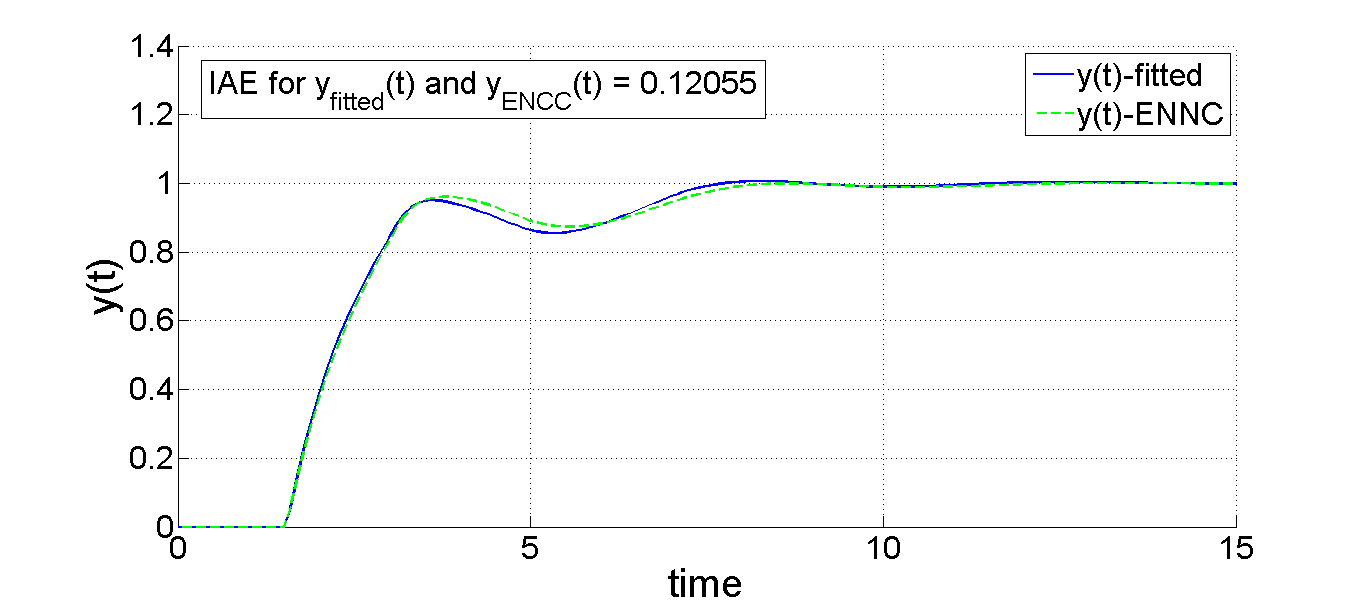
\includegraphics[width=0.8\columnwidth]{servo2.png}
	\caption{Servo response for the Pareto results found with the \gls{nnc} method and the tuning results.}
	\label{F:firstsim}
\end{figure}
%
The step response of the control signal is shown in Figure~\ref{F:u1} while the comparison for an input-disturbance is presented in Figure~\ref{F:di1} and for the output disturbance is in Figure~\ref{F:do1}. 
%
\begin{figure}[tb]
	\centering
	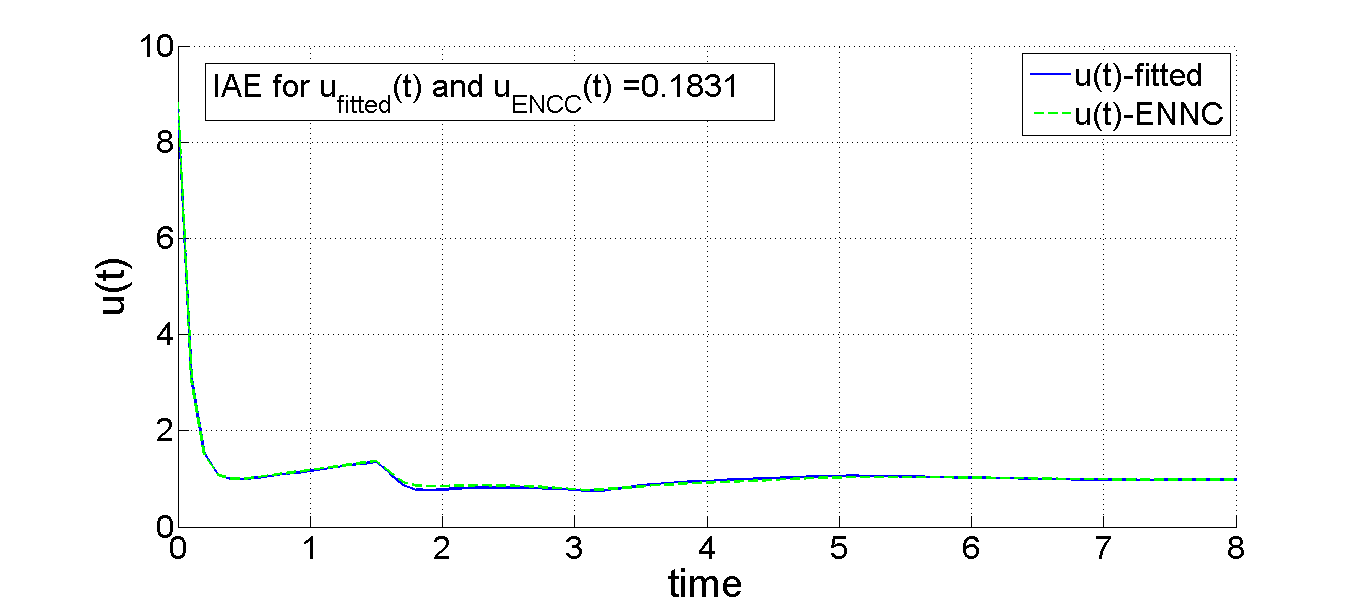
\includegraphics[width=0.8\columnwidth]{u2.png}
	\caption{Comparison of the control action  signal for a setpoint step change using the data from the Pareto found with the \gls{ennc} method and the tuning rule.}
	\label{F:u1}
\end{figure}
%
\begin{figure}[tb]
	\centering
	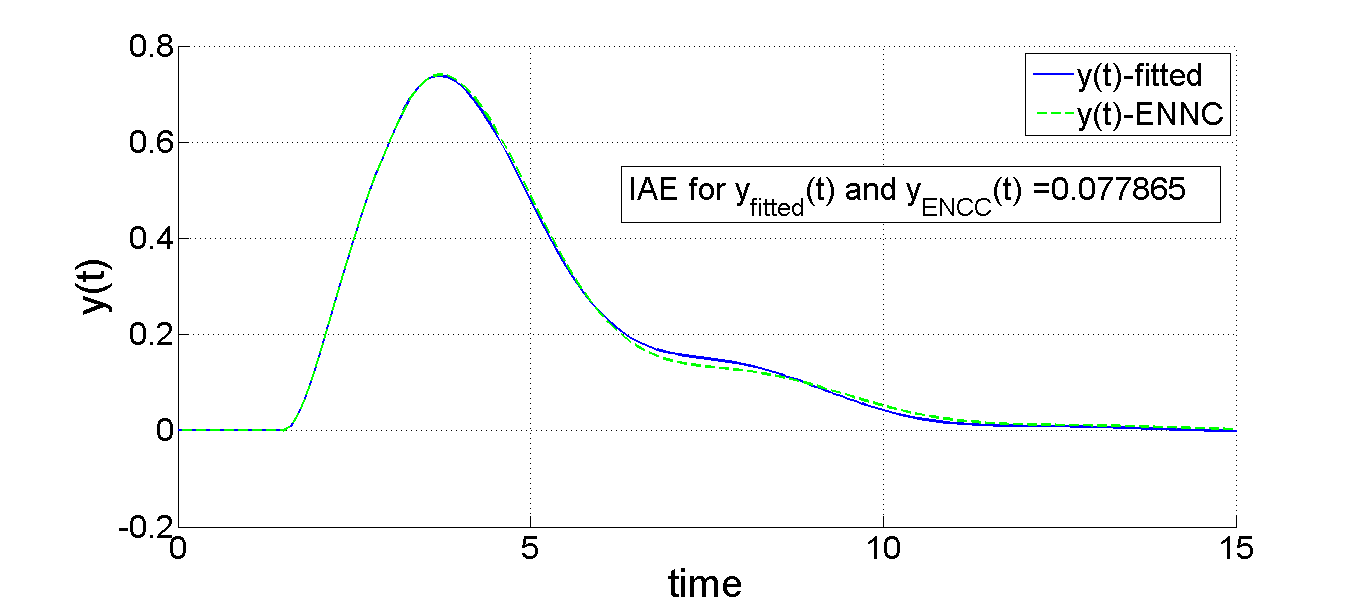
\includegraphics[width=0.8\columnwidth]{di2.png}
	\caption{Step input disturbance response for tuning from Pareto (ENNC method) and regressions results.}
	\label{F:di1}
\end{figure}
%
\begin{figure}[tb]
	\centering
	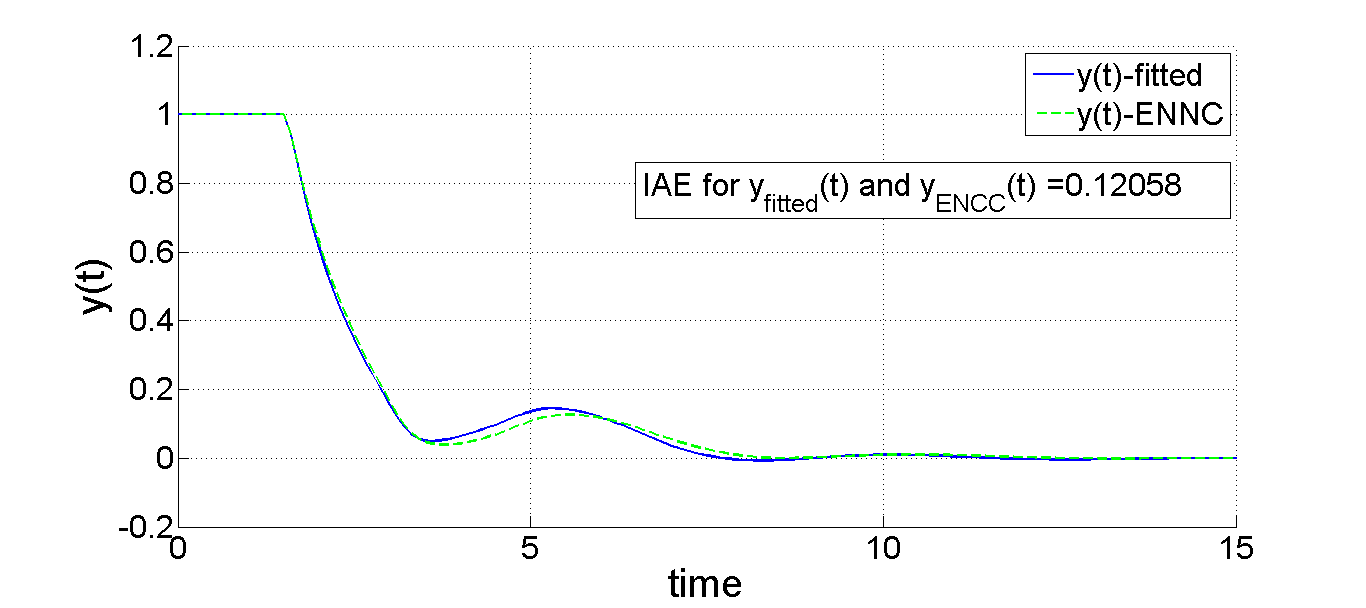
\includegraphics[width=0.8\columnwidth]{do2.png}
	\caption{Step output disturbance response for ENNC results and regressions results.}
	\label{F:do1}
\end{figure}
%
The figures show the \gls{iae} between both signals as a measure of how good the tuning rule approximates the optimization. As it can be seen, the responses are almost identical, showing that this methodology is feasible.

The tuning rule is also used for the extreme cases of $\tau_0$, that is, $\tau_0=1$ and $\tau_0=2$, using the following models:
%
\begin{equation}
P_F(\hat{s}) = \frac{e^{-\hat{s}}}{(\hat{s}+1)(0.5\hat{s}+1)},
\label{E:p2}
\end{equation}
%
\begin{equation}
P_S(\hat{s}) = \frac{e^{-2\hat{s}}}{(\hat{s}+1)(0.5\hat{s}+1)},
\label{E:p3}
\end{equation}
%
where $P_F(\hat{s})$ and $P_S(\hat{s})$ stand for the minimum and maximum  dead time considered in this study, respectively.

The allowed degradation was set to $\delta = 0.5$ and $\gamma = 0.5$. As before, one would expect to have the best servo response that complies with the allowed degradation. The comparison between the Pareto optimizations and the tuning rule for $P_F$ and $P_S$ are shown in Table~\ref{T:T2} and Table~\ref{T:T3} respectively.
%
\begin{table}[tb]
	\centering
	\caption{Results for $J_{di}$, $J_{do}$ and $J_{r}$, using $\delta = 0.5$ and $\gamma = 0.5$ for $P_F(s)$.}
	\label{T:T2}
	\begin{tabular}{@{}K{0.2\columnwidth} K{0.2\columnwidth} K{0.2\columnwidth} K{0.2\columnwidth}@{}}
		\toprule
		$\bm{\theta}$ and IAE & From tuning rule & From Pareto & Difference (\%)\\
		\midrule
		$\kappa_p$	& $1.150$ 	& $1.120$ & $2.67$\\
		$\tau_i$ 	& $1.987$ s & $1.900$ s & $4.58$\\
		$\tau_d$ 	& $0.425$ s & $0.495$ s & $-14.14$\\
		$\beta$ 	& $0.887$ 	& $0.889$ & $-0.23$\\
		$J_r$ 		& $1.955$ 	& $2.1446$ & $8.84$\\
		$J_{di}$ 	& $1.729$ 	& $1.6947$ & $2.02$\\
		$J_{do}$ 	& $1.874$ 	& $1.803$ & $3.94$\\
		$M_s$		& $2.024$	& $2.013$ & $0.55$\\
		\bottomrule
	\end{tabular}
\end{table} 
%
\begin{table}[tb]
	\centering
	\caption{Results for $J_{di}$, $J_{do}$ and $J_{r}$, using $\delta = 0.5$ and $\gamma = 0.5$ for $P_S(s)$.}
	\label{T:T3}
	\begin{tabular}{@{}K{0.2\columnwidth} K{0.2\columnwidth} K{0.2\columnwidth} K{0.2\columnwidth}@{}}
		\toprule
		$\bm{\theta}$ and IAE & From tuning rule & From Pareto & Difference (\%)\\
		\midrule
		$\kappa_p$	& $0.742$	& $0.744$	& $-0.270$\\
		$\tau_i$ 	& $2.345$ s	& $2.264$	& $3.578$\\
		$\tau_d$ 	& $0.629$ s	& $0.712$	& $11.657$\\
		$\beta$ 	& $0.919$	& $0.927$	& $-0.863$\\
		$J_r$ 		& $3.360$	& $3.662$	& $-8.247$\\
		$J_{di}$ 	& $3.162$	& $3.065$	& $3.165$\\
		$J_{do}$ 	& $3.237$	& $3.158$	& $2.502$\\
		$M_s$		& $1.976$	& $2.000$	& $-0.012$\\
		\bottomrule
	\end{tabular}
\end{table}

It is clear that the tuning rule is able to produce near Pareto-optimal controllers (in both cases, the maximum error is in $\tau_d$).

One of the interesting features is that the decision maker is able to choose the final solution by given a suitable value to $\delta$ and $\gamma$ as he or she considers appropriate. Since the data used to find the tuning rule had the constraint to have a maximum sensitivity of $M_s =2.0$ it is expected to have a stable closed-loop. Another interesting characteristic of this tuning rule is its ability to select the appropriate parameters taking into account three different sources of disturbances, unlike other \gls{pid} tuning rules.

From Table~\ref{T:T2} and \ref{T:T3} it can be deduced that the tuning rule finds a controller that has a better servo response than using the data directly, but compromising the response to the input and output disturbance rejection.

\subsection{Comments on creating tuning rules from Pareto fronts}
\label{sec:TuningRules}
With the example presented above, it was clear that it is feasible to find tuning rules from Pareto fronts. However, there are several points that need to be addressed:
\begin{itemize}
	\item The tuning rule was intended to be as simple as possible. However, it needed 126 coefficients to find the four parameters of the controller. Compared with other tuning rules \cite{odwyer2006}, this tuning rule is complex.
	%
	\item The idea of the degradation factor is interesting and directly related to the Pareto front, however, is not as intuitive as setting something more measurable, as the time constant of the closed-loop system for example.
	%
	\item The tuning rule is restricted to values of $1 \leq \tau_0 2$. The data for other values of $\tau_0$ exist, in fact, the reader can download the complete set of data from the companion software for this book. However, the complexity of the data made unfeasible to find a good simple tuning rule for all possible values of $\tau_0$.
	%
	\item The tuning rule is also restricted to PID controllers. But it is very common to use PI controllers in the industry. However, it is not possible to just discard the derivative time from the obtained tuning.
	%
	\item The data obtained from the optimizations has the contraint to have certain Maximum Sensitivity $M_s$. However, the presented rule takes into account only the value of $M_s = 2$. In order to have tuning rules for other values of $M_s$, possibly another set of 126 coefficients needs to be found for each desired value, which requires a lot of effort that may be not worth it.
\end{itemize}

All these points raise an important question, is it useful to find tuning rules that becomes too cumbersome for setting a PID controller? The literature about PID tuning (see \cite{ODwyer2000} for a list of PID tuning rules) generally shows simple tuning rules that need only a few decision parameters (for example \cite{Skogestad2003}) or even no decision parameters, since they minimize a single cost function (as in the MoReRT tuning rule \cite{Alfaro2016}), and therefore, only one tuning is possible. However, using the multiobjective approach presented here, the relationships between the controller gains, the tuning parameters and the model parameters become so complex, that a simple tuning rule that compasses all cases is impossible to find.

In these case, a more direct approach may be more suitable for the task of finding the best controller tuning. It is true that the Pareto front is not the final solution for the tuning problem, however only a selection is needed to ultimately find the desired solution. Therefore, a \textit{database} approach may be more sensible to the task at hand. This option is explored in the next section.
%
\section{Database approach for the final tuning}
\label{sec:DatabaseMOOP}
%

%
\chapter{Industrial application examples}
\label{chap:ApplicationExamples}
%
\abstract{In this chapter, different examples are provided to apply the tool presented in this book. The MOOTuning software is used to analyze the temperature control in a Continuous Stirred Tank Heater (CSTH) in Section~\ref{sec:CSTH} using two a three cost functions. Also a Continuos Stirred Tank Reactor (CSTR) is considered for the control of the concentration of the product in an isothermal case in Section~\ref{sec:CSTRVandeVusse}}
%

%
\section{Continuous Stirred Tank Heater}
\label{sec:CSTH}
%
\subsection{Description of the process}
\label{sec:DescriptionCSTH}
%
The control of a \gls{csth} is a common task in industrial processes. In this section, the control of the temperature of the \gls{csth} will be solved as a \gls{moop} using a \gls{2dof} \gls{pid} controller. The diagram of the process is presented in %
\begin{figure}[b]
	\centering
	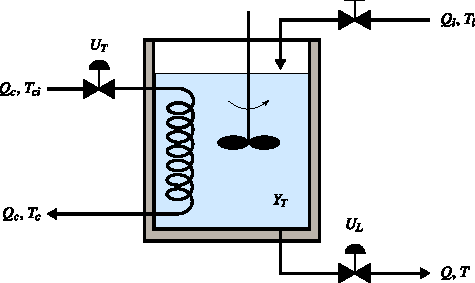
\includegraphics{Ch7CSTR}
	\caption{Simplified diagram of a continuous stirred-tank heater to be controlled.}
	\label{fig:Ch7CSTR}
\end{figure}
Figure~\ref{fig:Ch7CSTR}. A heat exchanger is installed inside the tank to heat the fluid. The flow rate inside the heat exchanger is controlled with a valve with input variable $U_T$ and the liquid inside the heat exchanger enters with temperature $T_{ci}$ and leaves with temperature $T_{co}$, the average temperature inide the heat exchanger is $T_{ca}$. The volume inside the tank is variable, the input flow rate is $Q_i$ with temperature $T_i$. The output flow rate is $Q$ with temperature $T$. The output flow rate is controlled with a valve with input variable $U_L$. The tank is covered with a jacket that prevents any heat loss to the atmosphere.

According to \citet{Alfaro2016}, a possible model for this process is given by the following set of algebraic-differential equations:
\begin{itemize}
	\item Tank mass balance:
			\begin{equation*}
				A \frac{d H(t)}{dt} = Q_i(t) - Q(t),
			\end{equation*}
			where $A$ is the transversal area of the tank and $H(t)$ is the liquid level.
	\item Tank energy balance:
			\begin{equation*}
				\rho C_p A H(t) \frac{T(t)}{dt} = \rho C_p Q_i(t)\left( T_i(t) - T(t)\right) + W(t),
			\end{equation*}
			where $C_p$ is the heat capacity of the fluid and $W(t)$ is the rate of heat transfer from the heat exchanger to the tank. $W(t)$ can be modeled as:
	\item Heat exchanger energy balance:
			\begin{equation*}
				\rho_c C_{pc} V_c \frac{T_{ca}(t)}{dt} = \rho_c C_{pc} Q_c(t)\left( T_{ci}(t)-T_{co}(t)\right) - W(t),
			\end{equation*}
			where $\rho_c$ is the density of the fluid inside the heat exchanger, $C_{pc}$ is the heat capacity of the fluid inside the heat exchanger and $V_c$ is the volume of the heat exchanger.
	\item Heat transfer between the heat exchanger and the fluid in the tank:
			\begin{equation*}
				W(t) = U A_c \left( T_{ca}(t) - T(t)\right), 
			\end{equation*}
			where $U$ is overall heat-transfer coefficient, $A_c$ is the area of the heat exchanger, $T_{ca}(t)$ is the average temperature inside the heat exchanger which is related to $T_{co}(t)$ and $T_{ci}(t)$ as:
			\begin{equation*}
				T_{ca}(t) = \frac{T_{ci}(t) + T_{co}(t)}{2}
			\end{equation*}
\end{itemize}

Also, in \citet{Alfaro2016}, the transmitters and the valves are modeled as:
\begin{itemize}
	\item Level transmitter: it is supposed that the level transmitter is a capacitive type electronic transmitter that has a first order dynamics:
		\begin{equation*}
			T_L \frac{d Y_L(t)}{dt} + Y_L(t) = K_L H(t),
		\end{equation*}
		%
		where $T_L$ is its time constant, $Y_L$ is the level signal and $K_L$ is the transmitter gain.
	%
	\item Temperature transmitter: It is supposed that a Pt$_{100}$ RTD electronic sensor is installed in a thermowell at the tank outlet pipe. It is supposed that it has a second order dynamic:
	%
		\begin{equation*}
			T_{T}^2 \frac{d^2 Y_T(t)}{dt^2} + 2T_T \frac{d Y_T(t)}{dt} + Y_T(t) = K_T T(t),
		\end{equation*}
		%
		where $T_T$ is its time constant and $K_T$ is its gain.
	%
	\item Level control valve: it is supposed that a ball valve with an electroneumatic actuator is used. The valve	inherent flow characteristics is nearly quadratic and the relationship between the flow $Q(t)$ and the input variable $U_L$ is given by:
		\begin{align*}
			T_{vL} \frac{d X_L(t)}{dt} + X_L(t) = K_{xL} U_L(t),\\
			Q(t) = K_{vL} X_L^2(t)\sqrt{\rho g H(t)},
		\end{align*}
		where $T_{vL}$ is the level control valve time constant, $K_{xL}$ level control valve stem constant $K_{vL}$ level control valve constant and $X_L(t)$ is the level control valve stem normalized travel.
	%
	\item Temperature control valve it is also supposed to be a ball valve with an electroneumatic actuator, however, it is supposed that the valve has an equal-percentage inherent flow characteristics given by:
		\begin{align*}
			T_{vT} \frac{d X_T(t)}{dt} + X_T(t) = K_{xT} U_T(t),\\
			Q_c(t) = K_{vT}R_{vT}^{\left( X_T(t) -1 \right) } \sqrt{P_{cp} - \left(R_c Q^2_c(t)+P_{cr} \right) },
		\end{align*}
		where $T_{vT}$ is the temperature control valve time constant, $K_{xT}$ the temperature control valve stem constant, $K_{vT}$ is the temperature control valve constant $P_{cp}$ is the heating fluid pump discharge pressure, $P_{cr}$ is heating fluid system return pressure and $X_T(t)$ is the temperature control valve stem normalized travel.
\end{itemize}

Taking this model in consideration, it can be said that, from the point of view of the controller, the controlled variables are give by the signals $Y_L(t)$ (which represents the level) and $Y_T(t)$ (which represents the temperature of the fluid of the tank). The manipulated variables are given by $U_L(t)$ (which directly affects $Q$) and $U_T(t)$ (that directly affects $Q_{c}$). $Q_i(t)$, $T_i$ and $T_{ci}$ are considered as disturbances. The state variables of the system are given by $H(t)$, $T_T(t)$, $T_{co}$, $Y_L(t)$, $Y_T$, $X_L(t)$ and $X_T(t)$, therefore, this model comprises a seventh order non-linear system for a two-input two-output industrial process. The parameters of the model can be found in 
\begin{table}
	\centering
	\caption{Parameters for the CSTH process}
	\label{tab:ParametersCSTH}
	\begin{tabular}{ccc}
		\toprule
		\textbf{Symbol} & \textbf{Value} & \textbf{Description}\\
		\midrule
		\multicolumn{3}{c}{\textbf{\textit{Tank parameters}}}\\
		\midrule
		$\rho$ 		& \SI{1200}{\kilogram\per\meter\cubed} 			& tank fluid density\\
		$A$			& \SI{0.0707}{\square\meter}					& tank inside section area\\
		$C_p$		& \SI{4190}{\joule\per\kilogram\per\celsius}	& tank fluid heat capacity\\
		$g$			& \SI{9.8}{\meter\per\square\second}			& gravity acceleration\\
		$K_T$		& \SI{2}{\%\per\celsius}						& temperature transmitter gain\\
		$K_{vL}$	& \num{1.25e-5}									& level control valve constant\\
		$K_{vT}$	& \num{3e-6}									& temperature control valve constant\\
		$K_{xL}$	& \SI{0.01}{\per\%}								& level control valve stem constant\\
		$Q_i$		& \SI{7e-4}{\cubic\meter\per\second}			& normal tank inlet fluid flow rate\\
		$T_i$		& \SI{24}{\celsius}								& fluid inlet temperature\\
		$T_L$		& \SI{2}{\second}								& level transmitter time constant\\
		$T_T$		& \SI{15}{\second}								& temperature transmitter time constant\\
		$T_{vL}$	& \SI{3}{\second}								& level control valve time constant\\
		$T_{vT}$	& \SI{5}{\second}								& temperature control valve time constant\\
		\midrule
		\multicolumn{3}{c}{\textbf{\textit{Heat exchanger parameters}}}\\
		\midrule
		$\rho_c$ 	& \SI{800}{\kilogram\per\meter\cubed} 			& heating fluid density\\
		$A_c$		& \SI{0.6362}{\square\meter}					& heat exchanger transfer area\\
		$C_{pc}$	& \SI{2400}{\joule\per\kilogram\per\celsius}	& heating fluid heat capacity\\
		$K_L$		& \SI{125}{\%\per\meter}						& level transmitter gain\\
		$K_{xT}$	& \SI{0.01}{\per\%}								& temperature control valve stem constant\\
		$P_{cp}$	& \SI{4.14e5}{\pascal}							& heating fluid pump discharge pressure\\
		$P_{cr}$	& \SI{1.38e5}{\pascal}							& heating fluid system return pressure\\
		$R_c$		& \SI{5.5e10}{\pascal\per(\cubic\meter\per\second)^2}	& heating system pipe nominal flow resistance\\
		$R_{vT}$	& \num{50}										& temperature control valve rangeability\\
		$T_{ci}$	& \SI{320}{\celsius}							& heating fluid inlet temperature\\
		$U$			& \SI{440}{\joule\per\second\per\square\meter\per\celsius}	& overall heat-transfer coefficient\\
		$V_c$		& \SI{0.0139}{\cubic\meter}						& heat exchanger volume\\
		\bottomrule
	\end{tabular}
\end{table}
%
Table~\ref{tab:ParametersCSTH}. This model was implemented in \simulink and can be found with the companion software. In %
%
\begin{figure}[tb]
	\centering
	\includegraphics[width=\columnwidth]{Ch7Implementation}
	\caption{\simulink implementation of the model of the heater.}
	\label{fig:Ch7Implementation}
\end{figure}
%
Figure~\ref{fig:Ch7Implementation}. Each equation of the model was implemented in a subsystem for clarity. For example in %
\begin{figure}
	\centering
	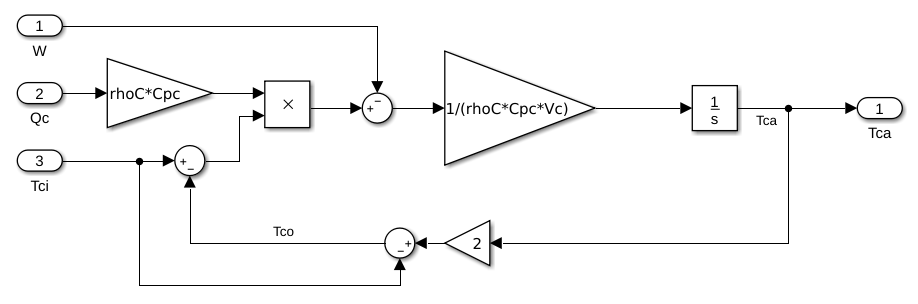
\includegraphics[width=\columnwidth]{Ch7HeatExhangerEq}
	\caption{Example of the implementation of the heat exchanger energy balance.}
	\label{fig:Ch7HeatExhangerEq}
\end{figure}
%
Figure~\ref{fig:Ch7HeatExhangerEq} the \simulink implementation of the heat exchanger energy balance is presented. The result of this submodel is the computation of the state variable $T_{ca}$, which represents the average temperature of the heating fluid. As it can be seen, the parameters of the model are not hard-coded in the \simulink blocks, instead a parameter initialization script is call before the simulation starts. If the user desires to change any value of the parameters, it can be done globally in the script and then automatically called during the simulation.

\subsection{Simplified linear model}
\label{sec:SimpLinMod}
In order to find a PID controller using the MOOTuning app, it is necessary to find a linear model of the plant in the operation point. An identification procedure was performed with a change of 10\% in the value of $U_T$ to find the transfer function between $Y_T$ and $U_T$. The response to this change is depicted in %
\begin{figure}[tb]
	\centering
	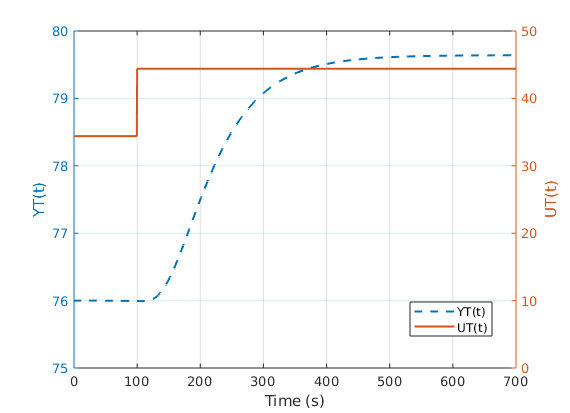
\includegraphics[width=\columnwidth]{Ch7CSTHResp}
	\caption{Response of the process to a change of 10\% in the $U_T(t)$ input.}
	\label{fig:Ch7CSTHResp}
\end{figure}
%
Figure~\ref{fig:Ch7CSTHResp}. As it can be seen, the response is overdamped and takes approximately \SI{500}{\second} to reach a new steady state. A change in 10\% on the input signal produces a variation of approximately $3.5\%$ in the output signal. It has to be noticed that the presented signals are normalized between 0 and 100\% representing the full spam of the transmitter and actuators.

In order to find the model, the process was supposed to have two poles, no zeros and a pure time-delay (also known as dead-time). Of course, if a linearization procedure were performed using the nonlinear model, a seventh order model would be obtained. However, for PID tuning, a first or second order model is usually expected to tune the controller.

Considering the experiment performed with the data as depicted in Figure~\ref{fig:Ch7CSTHResp}, the resulting simplified model is given by:
%
\begin{equation}
\frac{Y_T(s)}{U_T(s)} = \frac{0.3658 e^{-24.736 s}}{(52.861 s+1)(52.805 s +1)}.
\label{eq:TFCSTH}
\end{equation}

From this transfer function, it can be deduced that the gain is equal to $K = 0.3658$, the main time constant is given by $T = 52.861$, the ratio between the two time constant is given by $a = 0.9989$ and the dead-time is given by $L = 24.736$, therefore the normalized dead-time is given by $\tau = 0.4679$.

To test the validity of this simplified model, the response of the transfer function is compared against the response of the non-linear model. It was found that the transfer function response is very similar to the response of the non-linear model, as can be seen in %
%
\begin{figure}[tb]
	\centering
	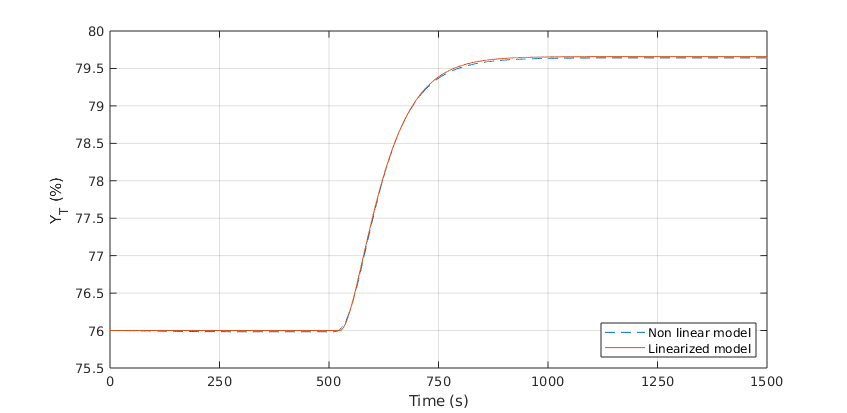
\includegraphics[width=\columnwidth]{Ch7CSTHComp}
	\caption{Comparison between the linear and no linear models for the CSTH.}
	\label{fig:Ch7CSTHComp}
\end{figure}
%
Figure~\ref{fig:Ch7CSTHComp}. It is clear that the non-linear model is a good representation of the dynamical response of the process. This is the first step in order to find a suitable PID controller to control the plant. In \citet{Alfaro2016} the level of the tank is also controlled, however the dynamic of the level is simpler (its model can be approximated with a first order model without delay) and in this particular example, only the temperature is going to be controlled, while the level is considered to be constant.
%
\subsection{PID control of the CSTH considering two integral cost functions}
\label{sec:PIDCSTH}
In this section, the process will be controlled using a \gls{pid} controller with different tuning methods and compared with the \gls{moo} framework used in the book.

Two different tuning rules were considered: the method by \citet{Rovira1969a} and the method by \citet{Murril1967}. For the case of the Rovira and Murril method, the model in \eqref{eq:TFCSTH} was reduced to a first order model using the Half-Rule in \citet{Skogestad2003}:
\begin{equation}
\frac{Y_T(s)}{U_T(s)} = \frac{0.3658 e^{-24.7360 s}}{79.2635 s +1}.
\label{eq:TFCSTHFirstOrder}
\end{equation}

The equations were implemented as presented in \citet{odwyer2006}:
\begin{itemize}
%	\item SIMC method: Supposing a \gls{soptd} model:
%			\begin{equation*}
%				P(s) = \frac{K e^{-Ls}}{(Ts+1)(aTs+1)}
%			\end{equation*}
%			The corresponding PID tuning for a closed-loop lag time of $T_c = L$ and the case where $T \leq 8 L$, the PID tuning is given by:
%			\begin{align*}
%				K_p &= \frac{0.5}{K}\frac{(1+a)T}{L}\\
%				T_i &= (1 + a) T\\
%				T_d	&= \frac{a}{1+a}T
%			\end{align*}
%	%
	\item Supposing a \gls{foptd} model given by:
			\begin{equation*}
				P(s) = \frac{K e^{-L s}}{Ts+1}
			\end{equation*}
			The Murrill tuning is given by:
				\begin{align*}
					K_p &= \frac{1.435}{K}\left( \frac{T}{L} \right)^{0.921}\\
					T_i &= \frac{T}{0.878}\left( \frac{L}{T}\right)^{0.749}\\\\
					T_d &= 0.482 T \left( \frac{L}{T} \right)^{1.137}
				\end{align*}
	\item Again, supposing a \gls{foptd} as above, the Rovira tuning is given by:
			\begin{align*}
				K_p &= \frac{1.086}{K} \left( \frac{T}{L}\right) ^{0.869} \\
				T_i &= \frac{T}{0.740 - 0.13\frac{L}{T}} \\
				T_d &= 0.384 T \left( \frac{L}{T}\right)^{0.914} 
			\end{align*}
\end{itemize}

The values of the computed values can be found on %
\begin{table}[tb]
	\centering
	\caption{Comparison of different PID tunings for the CSTH process.}
	\setlength{\tabcolsep}{8pt}
	\begin{tabular}{ccccccc}
		\toprule
		Tuning 	& $K_p$ 	& $T_i$		& $T_d$		& $\beta$	& $J_{r}$	& $J_{di}$\\
		\midrule
		%
		%SIMC	& $5.84$	& $105.67$	& $26.42$	& $1$			& $55.14$	& $18.10$\\
		Murril	& $5.87$	& $65.02$	& $23.21$	& $1$			& $82.51$	& $15.34$\\
		Rovira	& $4.34$	& $120.81$	& $18.48$	& $1$			& $76.00$	& $27.79$\\
		MOO01	& $11.3$	& $58.82$	& $29.48$	& $0.43$		& $85.65$	& $7.06$\\
		MOO02	& $9.26$	& $123.85$	& $26.68$	& $0.80$		& $69.96$	& $13.38$\\
		MOO03	& $8.20$	& $185.21$	& $28.14$	& $0.99$		& $67.93$	& $22.54$\\
		\bottomrule
	\end{tabular}
	\label{tab:CompPIDCSTH}
\end{table}
%
Table~\ref{tab:CompPIDCSTH}, along with its associated values of $J_{di}$ and $J_r$. The Murril and Rovira methods presented in the table were selected because they are intended to minimize the \gls{iae}. In all cases, the PID tuning is for a one degree of freedom controller (that is  the reason why $\beta$ is equal to one).

The PID that can be found using the data and the framework presented in Chapter~\ref{chap:PIDMOOP} is a \gls{soptd}, which may do the comparison somehow unfair. However, the idea now is to compare methods that tries to minimize the \gls{iae}. Using the MOOTuning Tool that accompanies this book, the Pareto front that was found is given as in %
%
\begin{figure}[tb]
	\centering
	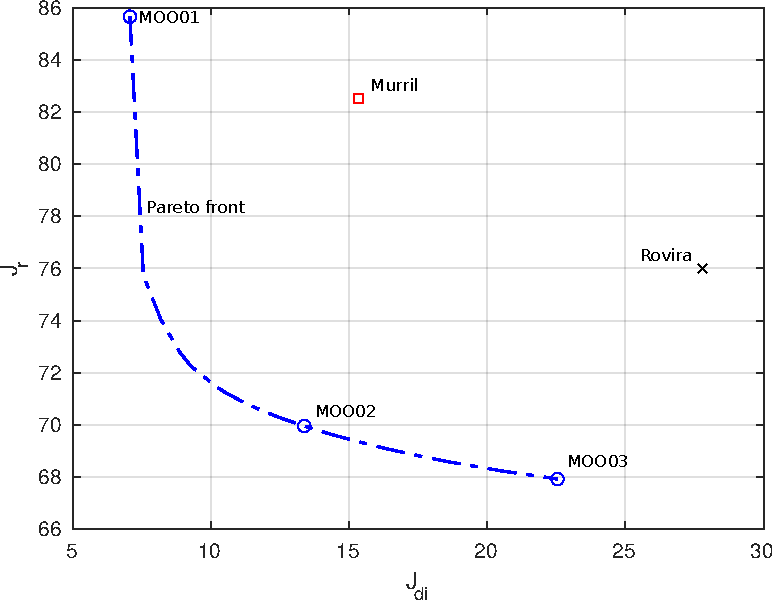
\includegraphics[width=\columnwidth]{Ch7CompPareto}
	\caption{MOOTuning compared to the Murril and Rovira methods that also minimizes \gls{iae}.}
	\label{fig:Ch7CompPareto}
\end{figure}
%
Figure~\ref{fig:Ch7CompPareto}. As it was expected, all the controllers found using the \gls{moo} tool present lower values for $J_{di}$ and $J_r$. If all controllers had the same topology, most certainly both controller would be close to the anchor points. However, what it is important here is the fact that, using the tool, the user has the ability to chose between practically an infinity of possible controllers. From the Pareto front, three different tuning were selected in order to compare the responses using the non-linear plant. The values of the parameters are presented also in Table~\ref{tab:CompPIDCSTH} and depicted as circles in the Pareto front in Figure~\ref{fig:Ch7CompPareto}.
%
\begin{figure}[tb]
	\centering
	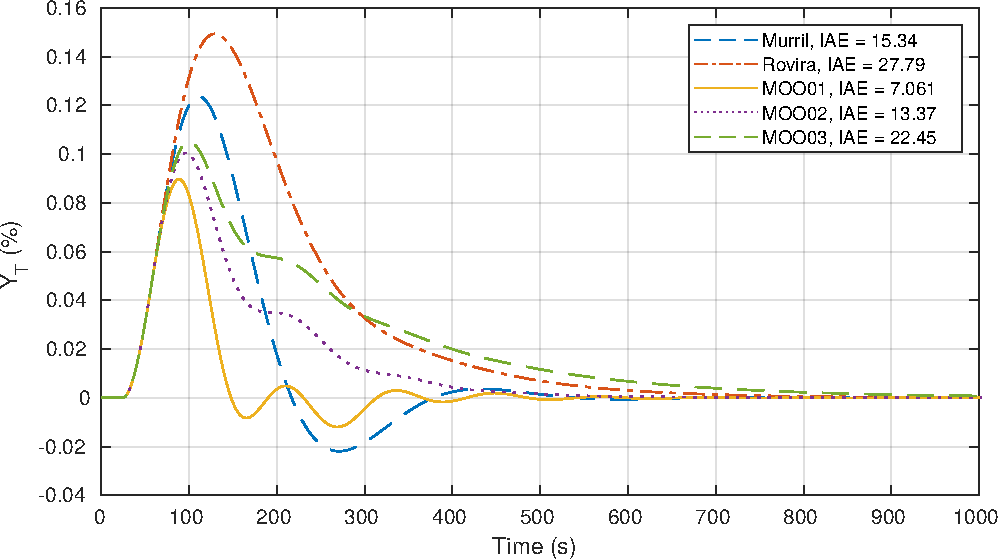
\includegraphics[width=\columnwidth]{Ch7CompParetoReg}
	\caption{Regulator response comparison for minimum IAE.}
	\label{fig:Ch7CompParetoReg}
\end{figure}
%
\begin{figure}[tb]
	\centering
	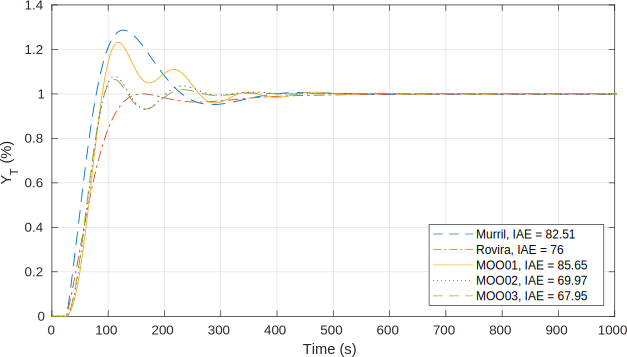
\includegraphics[width=\columnwidth]{Ch7CompParetoServo}
	\caption{Servo response comparison for minimum IAE.}
	\label{fig:Ch7CompParetoServo}
\end{figure}

In Figures~\ref{fig:Ch7CompParetoReg} and \ref{fig:Ch7CompParetoServo} the responses to a step change in the setpoint and in the disturbance are presented. The corresponding values of \gls{iae} are also presented in the graph. In all cases, the robustness was not considered as a constraint. but it is possible to include it within the MOOTuning software. From Figure~\ref{fig:Ch7CompPareto} given the steep slope of the curve for lower values of $J_{di}$ that a small change in $J_{di}$ may improve substantially the performance for $J_r$. Therefore, one may be more prone to select a controller that may have a little degradation in $J_{di}$ and for this reason, controller MOO01 may not be a good selection as a final solution unless having the minimum value possible of $J_{di}$ is the final goal.

The controller MOO02 may be seen as an intermediate solution between MOO1 and MOO03 in case both $J_{di}$ and $J_r$ are equally important for the decision maker. The power of the multiobjective framework is evident, and giving that the computational power is done offline, it becomes a good tool for the tuning of PIDs in an industrial setting.

To check how the tuning performs with the nonlinear model, a simulation was performed using the tuning of the controller $MOO02$. The setpoint was increased by $5\%$ at $t=\SI{100}{\second}$ and the temperature of the steam was increased by $\SI{10}{\celsius}$ at $t=\SI{700}{\second}$. The response is presented in %
\begin{figure}[tb]
	\centering
	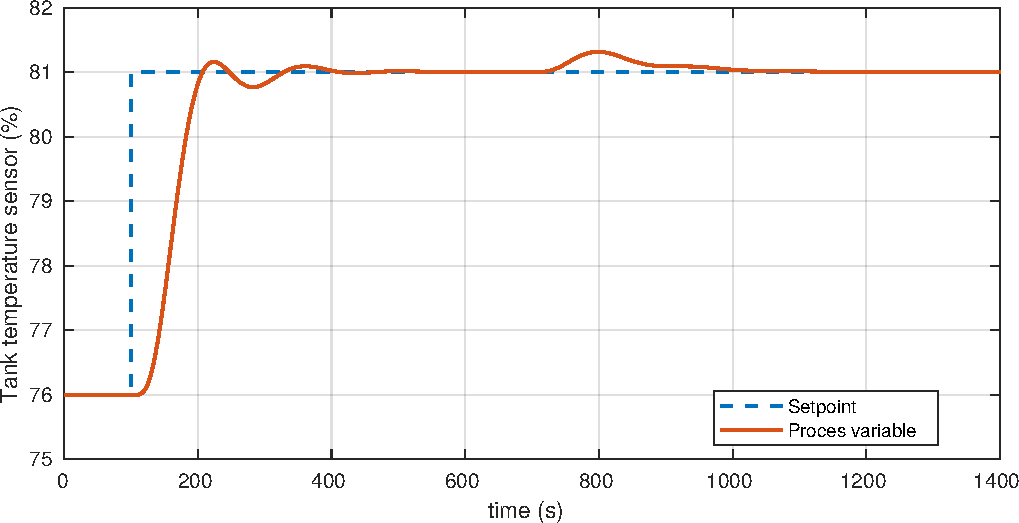
\includegraphics[width=\columnwidth]{Ch7CSTRControlled}
	\caption{Response of the controlled system using the nonlinear model for the CSTH.}
	\label{fig:Ch7CSTRControlled}
\end{figure}
%
Figure~\ref{fig:Ch7CSTRControlled}. As it can be seen, the servo response is very close to the one presented in Figure~\ref{fig:Ch7CompParetoServo}, which is a clear indicator that the linear model was a good approximation of the plant at the given operation point. The response to the change in the stem temperature cannot be compared with the regulation presented in Figure~\ref{fig:Ch7CompParetoReg}, because the disturbance was not applied directly in the input of the plant. However, it is interesting to note that the controller was able to respond with a good dynamic even though it was not optimize for this case.

The controlled variable is presented in %
\begin{figure}[tb]
	\centering
	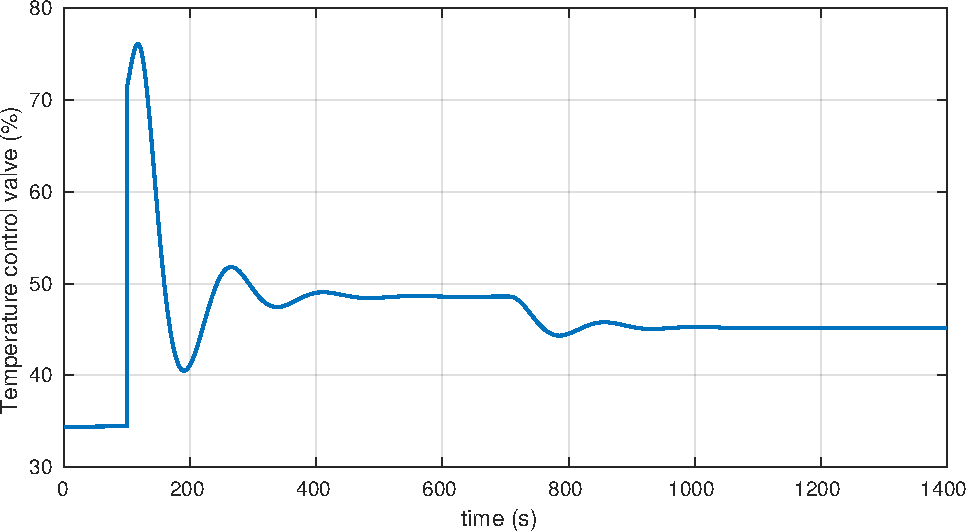
\includegraphics[width=\columnwidth]{Ch7CSTRControlledCV}
	\caption{Response of the controlled system using the nonlinear model for the CSTH.}
	\label{fig:Ch7CSTRControlledCV}
\end{figure}
%
Figure~\ref{fig:Ch7CSTRControlledCV}. When the setpoint change, the response of the controller is abrupt (more than double its original value), but then the value rapidly reach the new setpoint. The change produced by the disturbance has a milder response, and in less than \SI{200}{\second} reach again a new steady state.

The case presented here tried to show the steps to use the Pareto front as the methodology to find the controller tuning more appropriate to the task. The example is a simple plant, but very representative of the dynamics that can be found in an industry environment. Many of the plants can be modeled as a second order overdamped process, and therefore, the tool and the data used in this book are readily applied in many cases.

\subsection{PID control of the CSTH considering three integral cost functions}
\label{sec:PIDCSTH3Fun}
The MOOTuning software also is able to find the optimal parameters of a PID controllers considering three cost functions as presented in Section~\ref{sec:Tuning3PID}. Of course, it is not necessary to use this software since the data base with all the values is also part of the companion software, but the \matlab app has the advantage to be a simple interface between the user and the data.

As an example, the tuning tool is used to find the parameters of the controller that has the lowest $J_{do}$ value. This case is interesting because the anchor point where $J_{do}$ has the lowest value, neither the value of $J_r$ nor $J_{di}$ have their maximum value. On the other hand, when $J_{r}$ is set to be the lowest possible value, $J_{do}$ becomes the function that has an intermediate value but $J_{di}$ has its maximum value from the Pareto. Only for the anchor point where $J_{di}$ is minimum, both $J_r$ and $J_{do}$ get their maximum value. The responses for the three anchor points are depicted %
\begin{figure}[tb]
	\centering
	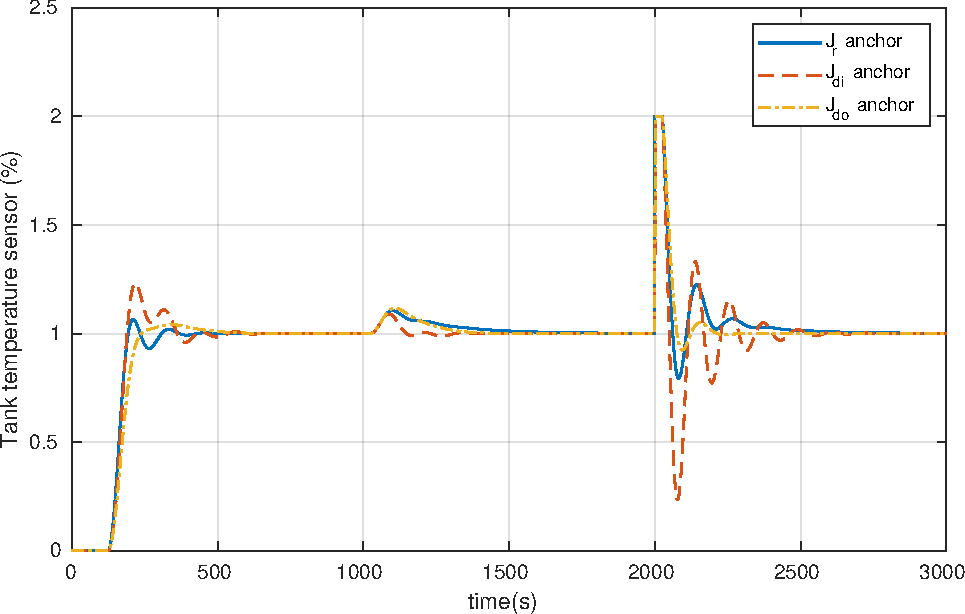
\includegraphics[width=\columnwidth]{Ch7CSTHControlled3Fun}
	\caption{Response of the CSTH process in the three anchor points of the pareto front for $M_s \leq 2.0$.}
	\label{fig:Ch7CSTHControlled3Fun}
\end{figure}
%
in Figure~\ref{fig:Ch7CSTHControlled3Fun} for the case where $M_s \leq 2.0$. As it can be seen, the response is quite different among the three anchor points. First a change in the reference value is performed at $t=\SI{100}{\second}$, an input step disturbance is present at $t=\SI{1000}{\second}$ and an output step disturbance is introduced in the system at $t=\SI{2000}{\second}$. The values of the cost functions are presented in %
%
\begin{table}
	\centering
	\caption{Cost functions for the three cost functions case scenario.}
	\begin{tabular}{cccc}
		\toprule
		 				& $J_r$ anchor point 					& $J_{di}$ anchor point				&	$J_{do}$ anchor point	\\
		 \midrule
		 $J_r$			&		$67.95$	(minimal)				&		$85.63$	($+26.02\%$)		&	$82.46$($+21.35\%$) \\
		 $J_{di}$		&		$22.46$ ($+218.13\%$)			&		$7.06$	(minimal)			&	$17.63$ ($+149.72\%$)	\\
		 $J_{do}$		&		$74.25$ ($+38.01\%$)			&		$102.43$ ($+90.39\%$)		&	$53.80$	(minimal)				\\
		 Parameters		& \begin{tabular}{c} $K_p = 8.19$ \\ $T_i = 185.18$\\ $T_d = 28.14$\\ $\beta = 0.99$		 \end{tabular} &
		 \begin{tabular}{c} $K_p = 11.29$ \\ $T_i = 58.8306$\\ $T_d = 29.48$\\ $\beta = 0.43$ \end{tabular} &
		 \begin{tabular}{c} $K_p = 6.18$ \\ $T_i = 108.76$\\ $T_d = 29.93$\\ $\beta = 0.82$ \end{tabular}\\
		 \bottomrule
	\end{tabular}
	\label{tab:2FunCostFunctionCSTH}
\end{table}
%
Table~\ref{tab:2FunCostFunctionCSTH}. The percentage increment is reported for each cost function in each case.

Using Figure~\ref{fig:Ch7CSTHControlled3Fun} and Table~\ref{tab:2FunCostFunctionCSTH} , it can be confirmed that the tuning with the best parameters for $J_{di}$ produces the worst responses for the other two functions. With these results one may be prone to select the tuning for the lowest value of $J_{di}$ as the final because it does not have the worst values of the other cost functions and it has much better response for the output disturbance case. Observe for example the response for the $J_{di}$ anchor point where the response for the output disturbance is bad (it has a $J_{do}$ increment of $+90.39\%$ with respect to its lowest value). In some sense, it could be seen as the best compromise between the cost functions. Only if the control engineer is heavily invested in minimize the $J_{di}$ cost function, it may select the $J_{di}$ anchor point as the final response, however, using the multiobjective framework presented here, he or she has to be fully aware that is selecting the worst response for the other functions.

Another reason to select the $J_{do}$ anchor point is related to the control effort. When the Total Variation computed as:
\begin{equation*}
TV = \sum_{i=0}^{N-1}\left(  u(i+1)-u(i)\right),
\end{equation*}
is compared between the three responses, it is found that $TV_{J_r} = 223.82$, $TV_{J_{di}} = 352.94$ and $TV_{J_{do}} = 152.81$ using a step size of $\SI{0.01}{\second}$. It is clear that the response given by the $J_{do}$ anchor point is a very good choice among all the possible values. The control signal is plotted %
%
\begin{figure}[tb]
	\centering
	\subfloat[Reference and input disturbance step changes.]{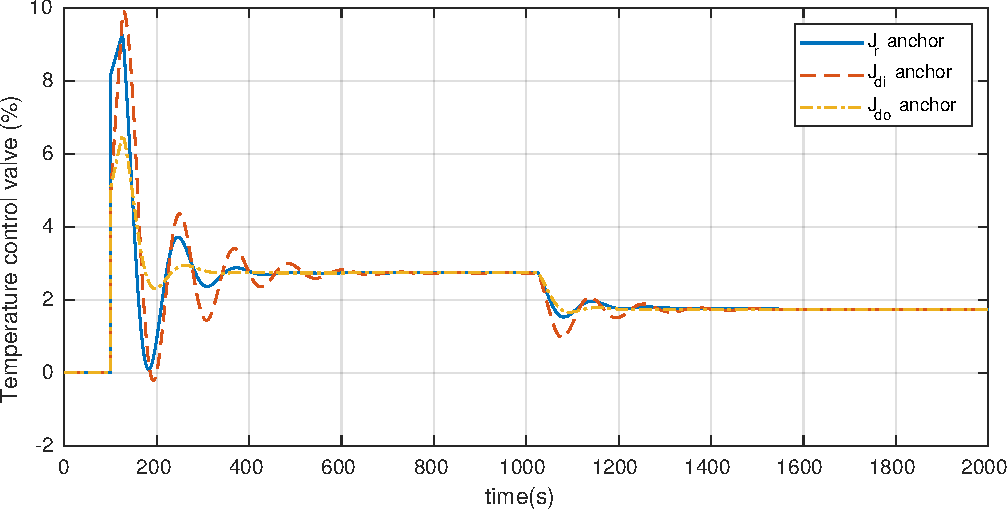
\includegraphics[width=\columnwidth]{Ch7CSTHControlledCV3Fun01} \label{fig:Ch7CSTHControlledCV3Fun01}}\\
	\subfloat[Output disturbance step change.]{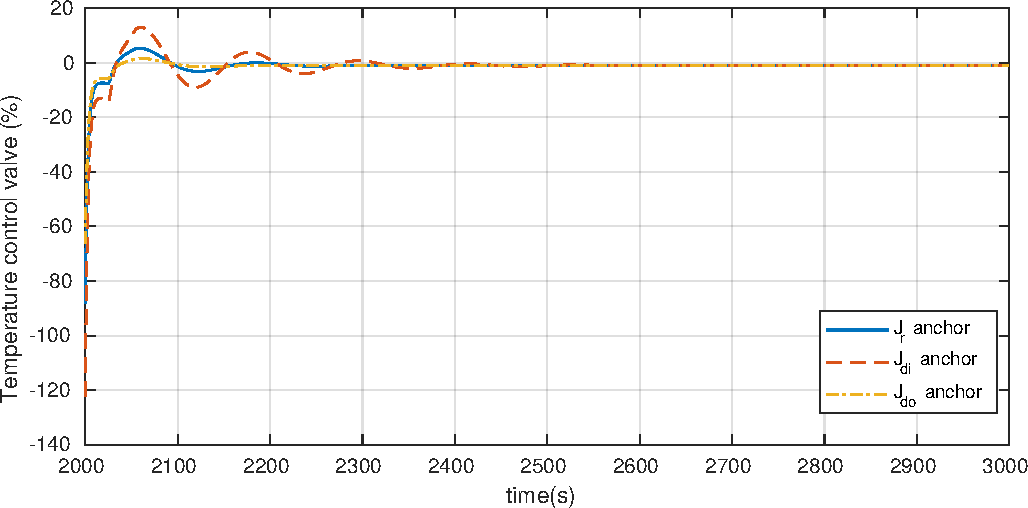
\includegraphics[width=\columnwidth]{Ch7CSTHControlledCV3Fun02} \label{fig:Ch7CSTHControlledCV3Fun02}}
	\caption{Control signal for the CSTH using three cost functions.}
	\label{fig:Ch7CSTHControlledCV3Fun}
\end{figure}
%
on Figure~\ref{fig:Ch7CSTHControlledCV3Fun}. Since the control signal has a larger magnitude for an output disturbance rejection, it was plotted in different axis.

As it can be seen from the response, effectively the response of the $J_{do}$ anchor point is smoother than the other two. Even if the control engineer is not looking for the best response to the output disturbance, the obtained tuning may be a good compromise between servo and regulation responses with a mild control signal.

In section~\ref{sec:PIDCSTH}, the system was controlled considering only two sources of disturbances. When adding another dimension to the problem, certainly the selection of the final controller may be more difficult because another degree of freedom is added. However, the insight that was gathered from rethinking the problem from this other point of view can be seen as beneficial, because the tuning found using the 3 dimensional Pareto could be a better solution (from a physical point of view) that may not be part of the front with only two functions.
%
% -----------------------------------------------------------------------------------------------------------
%
\section{Continuous Stirred Tank Reactor}
\label{sec:CSTRVandeVusse}
%
\subsection{Description of the process}
\label{sec:DescriptionCSTR}

The \gls{cstr} with the Van de Vusse reaction \citep{VandeVusse1964} is a common benchmark plant for testing control algorithms given its different dynamics depending on the operating point and is depicted in %
\begin{figure}[tb]
	\centering
	\includegraphics[scale=0.6]{Ch7VandeVusse}
	\caption{\gls{cstr} process using the Van de Vusse reaction model.}
	\label{fig:Ch7VandeVusse}
\end{figure}
%
Figure~\ref{fig:Ch7VandeVusse}. For this particular case, the isothermal process is considered and both the concentration sensor as the valve actuator will be modeled as well. The objective is to control the feed flow to obtain the desired concentration of a product.

The Van de Vusse reaction models a process where desired product B is obtained from A, but at the same time, both A and B are degraded to D and C respectively. The chemical equation that represent this reaction is given by:
%
\begin{align*}
A &\overset{k_1}{\longrightarrow} B \overset{k_2}{\longrightarrow}C,\\
2 A &\overset{k_3}{\longrightarrow} D,
\end{align*}
%
where $k_i$ are the rate constants of the formation rates of A and product B as given by \citep{VandeVusse1964}:
\begin{equation}
\begin{split}
r_A &= -k_1 A - k_3 A^2,\\
r_B &= k_1 A - k_2 B.
\end{split}
\label{eq:RateVandeVusse}
\end{equation}

When performing a mass balance, the model becomes \citep{Arrieta2010}:
%
\begin{equation}
\begin{split}
\frac{dC_A(t)}{dt} & = \frac{F_r(t)}{V} \left(C_{Ai}-C_A(t)\right) - k_1 C_A(t) - k_3 C^2_A(t)\\
\frac{dC_B(t)}{dt} & = -\frac{F_r(t)}{V} C_B(t)+ k_1 C_A(t) - k_2 C_B(t)
\end{split}
\label{eq:CSTRMVE}
\end{equation}
%
where $C_A$ and $C_B$ represents the reactants concentrations  in \si{\mole\per\liter}, $C_{Ai}$ is the concentration of A in the feed flow in \si{\mole\per\liter}, $F_r$ is the input flow in \si{\liter\per\minute}, and $V$ is the volume of the \gls{cstr} in \si{\liter}. The nominal values of the parameters are presented in %
%
\begin{table}[tb]
	\centering
	\caption{Parameters values for the \gls{cstr} model.}
	\begin{tabular}{cc}
		\toprule
		$k_1 = \SI{0.833}{\per\minute}$ & $k_2 = \SI{1.667}{\per\minute}$ \\
		$k_3 = \SI{0.167}{\per\minute}$ & $C_{Ai} = \SI{10}{\mole\per\liter}$\\
		$V = \SI{700}{\liter}$\\
		\bottomrule
	\end{tabular}
	\label{tab:ParamCSTR}
\end{table}
%

The range of the sensor for the product is supposed to be in the range 0 to \SI{1.5714}{\mole\per\liter} and the maximum flow that is allowed by the valve is given by \SI{634.1719}{\liter\per\minute}. Given these values, the model for the sensor-transmitter is given by:
\begin{equation}
	y(t) = \left(\frac{100}{1.5714}\right) C_B(t),
	\label{eq:Sensor}
\end{equation}
%
while the transmitter is modeled as:
\begin{equation}
F_r(t) = \left(\frac{634.1719}{100}\right) u(t),
\label{eq:Transmiter}
\end{equation}
%
where $u(t)$ and $y(t)$ are the normalized input and output signal, respectively. The operation point of the plant is given by $u_0 = 60\%$ and $y_0 = 70\%$ which represents concentration of $C_{A0} = \SI{2.9175}{\mole\per\liter}$ and $C_{B0} = \SI{1.10}{\mole\per\liter}$ with the input concentration given by $C_{Ai0} = \SI{10}{\mole\per\liter}$.

These parameters give the system a wide range of operation. In %
\begin{figure}
	\centering
	\includegraphics[width=\columnwidth]{Ch7VandeVusseOP}
	\caption{Operation points of the \gls{cstr} process.}
	\label{fig:Ch7VandeVusseOP}
\end{figure}
Figure~\ref{fig:Ch7VandeVusseOP} it can be seen that with the value of $C_{Ai0}$ given and the input at $60\%$, the output yield $70\%$. In the figure the dashed lines represents the variation due to $\pm 10\%$ variation of $C_{Ai}$. It can be seen that, with a $100 \%$ value for $u$ and a variation of $10\%$ of $C_{Ai}$, the output is less than $100\%$ of the capacity of the sensor.

The concentration of $C_a$ and $C_b$ are both plotted in %
\begin{figure}
	\centering
	\includegraphics[width=\linewidth]{Ch7VandeVusseOPStates}
	\caption{Concentration of the reactants for all possible operating points.}
	\label{fig:Ch7VandeVusseOPStates}
\end{figure}
%
Figure~\ref{fig:Ch7VandeVusseOPStates}. The $C_a$ concentration is on the horizontal axis is while the $C_b$ concentration is on the vertical axis. The selected operation point is represented with a circle in the curve and also the curves with the variation on the value of $C_{Ai}$ are also presented. As it can be seen, in the operation point selected, the curves start to diverge, which means that the model has a larger dependency on the variation of the input concentration. This has to be taken into account when designing the feedback controller.

When considering the transient response to a change in the input flow $u$, the response is as given in %
\begin{figure}
	\centering
	\includegraphics[width=\linewidth]{Ch7VandeVusseStep}
	\caption{Open loop response to a step change in the input signal of the \gls{cstr}.}
	\label{fig:Ch7VandeVusseStep}
\end{figure}
%
Figure~\ref{fig:Ch7VandeVusseStep}. It is interesting to note that the the system has an inverse response. This characteristic limits the possible performance of the controlled loop, making unfeasible to increase the gain of the controller to achieve a faster response without instability. This is also another point that has to be considered when designing the controller.

This model was implemented as an S-Function in \matlab/\simulink and can be found in the companion software. In %
\begin{figure}[tb]
	\centering
	\includegraphics[width=\linewidth]{Ch7CSTRSimulinkSystem}
	\caption{CSTR implemented as an S-function in \simulink.}
	\label{fig:Ch7CSTRSimulinkSystem}
\end{figure}
%
Figure~\ref{fig:Ch7CSTRSimulinkSystem}, the basic block with the model is presented. It has $u$ and $C_{ai}$ as inputs and $y$, $C_a$ and $C_b$ as outputs. With the intention to facilitate the characterization of the model, a mask was designed to enter the parameters and the initial value of the states. This mask can be found in %
\begin{figure}[tb]
	\centering
	\includegraphics[width=0.5\linewidth]{Ch7VandeVusseParamWindow}
	\caption{\simulink mask to enter parameters and initial values for the \gls{cstr} system.}
	\label{fig:Ch7VandeVusseParamWindow}
\end{figure}  
Figure~\ref{fig:Ch7VandeVusseParamWindow}. All the values of the parameters can be set on the \matlab workspace and use directly on the mask. This is and advantage in case the user desires to use another set of parameters or compare the response of the system with different values.

The objective of this example is to control the reactor using the multiobjective approach. In order to use the framework and the \matlab app, it is necessary to find a suitable linear second order model. Next, the procedure to find this model is presented.

\subsection{Linearization}
\label{sec:CSTRLin}
In order to use the MOOTuning software, it is necessary to have a linear model of the process. In this case, the linearization is done by taking the first order approximation of the model in \eqref{eq:CSTRMVE} near the operation point.

When defining the incremental variables $\mathbf{\delta x}$, $\mathbf{\delta u}$ and $\delta y$ as:
\begin{align*}
\mathbf{\delta x} &= \left[ \begin{array}{c} C_A - C_{A0} \\ C_B - C_{B0} \end{array} \right], \\
\mathbf{\delta u} &= \left[ \begin{array}{c} u-u_0 \\ C_{Ai} - C_{Ai0} \end{array} \right], \\
\delta y &= y - y_0 .
\end{align*}

The process dynamics can be approximated by the first order model given by:
%
\begin{align}
\dot{\mathbf{\delta x}} &=  \mathbf{A}\mathbf{\delta x} + \mathbf{B} \mathbf{\delta u}, \\
%
\delta y &=  \mathbf{C} \mathbf{\delta x},
\end{align}
%
where,
\begin{align*}
	\mathbf{A} &= \left[ \begin{array}{cc} \frac{6.341719 u_0}{V} - k1 - 2 k_3 C_{A0} & 0 \\ k1 & \frac{-6.341719 u_0}{V} - k_2 \end{array}\right],\\
	\mathbf{B} &= \left[ \begin{array}{cc} \frac{6.341719 (C_{Ai0}-C_{A0})}{V} & \frac{6.341719 u_0}{V} \\ \frac{-6.341719 C_{B0}}{V} & 0 \end{array} \right], \\
	\mathbf{C} &= \left[ \begin{array}{cc} 0 & \frac{100}{1.5714} \end{array} \right].
\end{align*}

Using the parameters of Table~\ref{tab:ParamCSTR} and the operation point values, the resulting transfer function between input $u$ and output $y$ is found to be:
\begin{equation}
	F(s) = \frac{-0.6342 s + 1.913}{s^2 + 4.56 s + 5.193}
	\label{eq:TFCSTR}
\end{equation}

It has to be clear that this transfer function is only an approximation of the model, and therefore it is valid only around the operating point. When a step change of $5\%$ is entered in the system, the response of the nonlinear model and the response of the transfer function start to differ as presented in %
%
\begin{figure}[tb]
	\centering
	\includegraphics[width=\linewidth]{Ch7CSTRLinear}
	\caption{Comparison of the nonlinear and linear model for the \gls{cstr} for a 5\% change in the input.}
	\label{fig:Ch7CSTRLinear}
\end{figure}
%
Figure~\ref{fig:Ch7CSTRLinear}. As it can be seen, the linear model represents the transient response well, however it fails to predict the steady state. Of course, the smaller the change in the input, the better is the the approximation for both the transient and the steady state response.

However, the model that is expected in the \matlab app does not contemplate a non-minimum phase zero in the model. Using the model reduction rules of \citet{Skogestad2003}, the \gls{soptd} model ends as:
\begin{equation}
	F_{aprox} = \frac{0.368 e^{-0.331}}{0.193 s^2 + 0.878 s +1}.
	\label{eq:Faprox}
\end{equation}
which corresponds to approximate the non-minimum phase zero by a time delay. The gain is given by $K=0.3684$, the time constant is given by $\tau= \SI{0.4256}{\minute}$, the time delay is $L= \SI{0.3315}{\minute}$ and $a = 0.9408$. This new transfer function gives the response presented in %
\begin{figure}[tb]
	\centering
	\includegraphics[width=\linewidth]{Ch7CSTRLinearSkogestad}
	\caption{Approximation of the non-minimum phase zero with a time delay for the linear model of the \gls{cstr}.}
	\label{fig:Ch7CSTRLinearSkogestad}
\end{figure}
%
Figure~\ref{fig:Ch7CSTRLinearSkogestad}. Of course, the dynamic model is quite different from the original nonlinear model, both in the transient and steady states. Since the controller is going to be designed with the linearized time-delayed transfer function, it is necessary to consider some restriction on the performance in order to give certain robustness to the design.

\subsection{Controller design}
For this particular example, the design of the controller parameters will contemplate three different robustness cases: without any restriction to the value of \gls{ms}, $M_s = 2.0$ and $M_s = 1.8$. The MOOTuning app is able to introduce the robustness as a restriction in the design. However, it is limited to certain values of $M_s$ which are considered to be reasonable for an industrial control applications.

In this particular example, only $J_{r}$ and $J_{di}$ are going to be considered. The design is based on the model in \eqref{eq:Faprox} and will be tested on the nonlinear model as well. Several points of the Pareto are going to be tested: the two anchor points (C1 for best regulator and C2 for best servo), the best regulator possible with a 20\% degradation on $J_r$ (C3) and the best servo possible with a 20\% degradation on $J_{di}$ (C4).
%
\begin{table}[tb]
	\caption{Different tunings for the \gls{cstr} obtained with MOOTuning.}
	\centering
	\begin{tabular}{m{1cm}m{1cm}m{1cm}m{1cm}m{1cm}m{1cm}m{1cm}}
		\toprule
		Design & $K_p$ & $T_i$ & $T_d$ & $\beta$ & $J_{di}$ & $J_r$ \\
		\midrule
		\multicolumn{7}{c}{$M_s \geq 2.0$} \\
		\midrule
		C1 & 6.00 & 0.61 & 0.29 & 0.49 & 0.13 & 0.98\\
		C2 & 4.54 & 1.24 & 0.26 & 0.99 & 0.27 & 0.80\\
		C3 & 5.54 & 0.85 & 0.26 & 0.66 & 0.14 & 0.85\\
		C4 & 5.33 & 0.91 & 0.26 & 0.73 & 0.17 & 0.84\\
		\midrule
		\multicolumn{7}{c}{$M_s = 2.0$} \\
		\midrule
		C1 & 4.43 & 0.76 & 0.21 & 0.66 & 0.17 & 0.92\\
		C2 & 4.29 & 1.19 & 0.25 & 0.99 & 0.28 & 0.80\\
		C3 & 4.44 & 0.86 & 0.22 & 0.73 & 0.19 & 0.86\\
		C4 & 4.40 & 1.00 & 0.24 & 0.87 & 0.23 & 0.83\\
		\midrule
		\multicolumn{7}{c}{$M_s = 1.8$} \\
		\midrule
		C1 & 3.88 & 0.72 & 0.22 & 0.72 & 0.20 & 0.98\\
		C2 & 3.86 & 1.13 & 0.24 & 0.99 & 0.29 & 0.82\\
		C3 & 3.91 & 0.85 & 0.21 & 0.75 & 0.22 & 0.89\\
		C4 & 3.92 & 0.96 & 0.22 & 0.87 & 0.24 & 0.85\\
		\bottomrule
	\end{tabular}
	\label{tab:CSTRDesigns}
\end{table}

All the tuning values for the cases studied are presented in Table~\ref{tab:CSTRDesigns}. In general, it can be seen that the proportional gain is heavily dependent of the robustness value (more robustness implies lower values of $K_p$). On the other hand it seems that the value of $T_i$ is more dependent of the degradation of $J_{di}$ while the variation of $T_d$ is small across all cases. The value of $\beta$ seems like a combination of the degradation of $J_{di}$ and the value of the robustness.

To compare the responses, it is useful to plot the step response of C1 controllers across all robustness values as presented in %
\begin{figure}[tb]
	\centering
	\includegraphics[width=\linewidth]{Ch7CSTRControlC1}
	\caption{Response for C1 controllers for all $M_s$ values.}
	\label{fig:Ch7CSTRControlC1}
\end{figure}
%
Figure~\ref{fig:Ch7CSTRControlC1} and for C2 controllers as in %
\begin{figure}[tb]
	\centering
	\includegraphics[width=\linewidth]{Ch7CSTRControlC2}
	\caption{Response for C2 controllers for all $M_s$ values.}
	\label{fig:Ch7CSTRControlC2}
\end{figure}
%
Figure~\ref{fig:Ch7CSTRControlC2}. It is interesting to note that C1 controllers presents more variability in the response with respect to the controllers of the C2 family. In both figures it is clear that there is a compromise between the servo and the regulator responses, but this compromise becomes less important when the robustness is considered. Consider Figure~\ref{fig:Ch7CSTRControlC1}, the response for $M_s \geq 2.0$ does not take into account any constraint on the robustness and as it can be seen this response is very different than the cases where $M_s = 2.0$ and $M_s = 1.8$ are forced. It has to be noticed that adding the robustness constraint greatly limits the possible values of the controllers.

On the other hand, it was found that for the C2 controllers family the responses are very similar among all robustness, as can be seen in Figure~\ref{fig:Ch7CSTRControlC2}. The reason for this is the parameter $\beta$. This parameter does not affect the robustness value of the controlled system nor the regulator response. Therefore, the optimization tend to find a low value for $K_p$, which gives better robustness, but then compensates with a high value of $\beta$.

The control signals for the controllers are presented in Figures~\ref{fig:Ch7CSTRControlC1U} and \ref{fig:Ch7CSTRControlC2U}. %
\begin{figure}[tb]
	\centering
	\includegraphics[width=\linewidth]{Ch7CSTRControlC1U}
	\caption{Control signal for C1 controllers for all $M_s$ values.}
	\label{fig:Ch7CSTRControlC1U}
\end{figure}
%
\begin{figure}[tb]
	\centering
	\includegraphics[width=\linewidth]{Ch7CSTRControlC2U}
	\caption{Control signal for C2 controllers for all $M_s$ values.}
	\label{fig:Ch7CSTRControlC2U}
\end{figure}
%
For the case of C1 controllers, the control signal varies significantly according to the robustness value. The case without any constraint has a larger peak and more oscillatory response than any of the other controllers. It is interesting, however, to note that the control signal for the C2 controllers are very similar and again, this is due to the presence of the $\beta$ parameter. The fact that an unconstrained controller may be applied to the controlled system has to be taken with caution, because in this design, the model used for the controller tuning is known to be different that the system. Therefore, applying an aggressive control signal may lead to unwanted oscillatory behavior and even instability.

Now, the responses of the different controllers families can be compared for the same given robustness, for example $M_s = 2.0$ as in %
\begin{figure}[tb]
	\centering
	\includegraphics[width=\linewidth]{Ch7CSTRControlMs2}
	\caption{Response for all controller families with $M_s = 2.0$.}
	\label{fig:Ch7CSTRControlMs2}
\end{figure}
%
Figure~\ref{fig:Ch7CSTRControlMs2}. For all this controllers, the robustness is near $M_s = 2.0$, but the performance is varied from $J_r$ and $J_{di}$. Here, the compromise between both responses is clearer since the best servo is at the same time the worst regulator and the best regulator is the worst servo.
%
\begin{figure}[tb]
	\centering
	\includegraphics[width=\linewidth]{Ch7CSTRControlMs2U}
	\caption{Control signal for all controller families with $M_s = 2.0$.}
	\label{fig:Ch7CSTRControlMs2U}
\end{figure}
%

However, given that all controllers are constraint to fulfill $M_s = 2.0$, the difference between them are not very notorious. It can be seen on Figure~\ref{fig:Ch7CSTRControlMs2U} that the peaks and oscillatory behavior of all controllers are practically the same. When the robustness became too thing (for example values below 1.4) the controllers for servo and regulator practically become the same and the degree of freedom to select the dynamic behavior is practically non-existent.

\subsection{Validation of the controller designs}
\label{sec:ValidationCSTR}
%
The designed controllers were tested using the nonlinear model of the \gls{cstr}. It is important to note that the controllers were tuned for a plant model that is different than the ``real'' plant. In this particular case, several approximations where made which were necessary in order to use the framework presented in the other chapters. Because of this, it is important to look for a solution that takes into account this possible sources of instability.
%
\begin{table}[tb]
	\centering
	\caption{IAE values for the controllers applied to the nonlinear model as servo controllers}
	\begin{tabular}{p{1.5cm}>{\centering}p{1cm}>{\centering}p{1cm}>{\centering}p{1cm}>{\centering\arraybackslash}p{1cm}}
		\toprule
		\multirow{2}{*}{Robustness}	& \multicolumn{4}{c}{Controller}\\
		\cmidrule{2-5}
									& C1 & C2 & C3 & C4 \\
		\midrule
		$M_s = 1.8$ & 0.94 & 0.83 & 0.87 & 0.84\\
		$M_s = 2.0$ & 0.86 & 0.79 & 0.83 & 0.81\\
		$M_s \geq 2.0$ & 11.20 & 0.78 & 1.02 & 0.83\\
		\bottomrule
	\end{tabular}
	\label{tab:CSTRIAEServo}
\end{table}
%
\begin{table}[tb]
	\centering
	\caption{TV values for the controllers applied to the nonlinear model as servo controllers}
	\begin{tabular}{p{1.5cm}>{\centering}p{1cm}>{\centering}p{1cm}>{\centering}p{1cm}>{\centering\arraybackslash}p{1cm}}
		\toprule
		\multirow{2}{*}{Robustness}	& \multicolumn{4}{c}{Controller}\\
		\cmidrule{2-5}
		& C1 & C2 & C3 & C4 \\
		\midrule
		$M_s = 1.8$ & 9.40 & 13.20 & 9.14 & 11.10\\
		$M_s = 2.0$ & 11.34 & 20.01 & 12.75 & 16.37\\
		$M_s \geq 2.0$ & 1936.10 & 29.10 & 128.30 & 73.20\\
		\bottomrule
	\end{tabular}
	\label{tab:CSTRTVServo}
\end{table}
%
\begin{figure}
	\centering
	\subfloat[$M_s = 2.0$]{\includegraphics[width=0.8\linewidth]{CH7CSTRControlServoMs2Y} \label{fig:CH7CSTRControlServoMs2Y}}\\
	\subfloat[$M_s = 1.8$]{\includegraphics[width=0.8\linewidth]{CH7CSTRControlServoMs18Y} \label{fig:CH7CSTRControlServoMs18Y}}\\
	\subfloat[$M_s \geq 2$]{\includegraphics[width=0.8\linewidth]{CH7CSTRControlServoMs10Y} \label{fig:CH7CSTRControlServoMs10Y}}
	\caption{Response of the controlled system with the nonlinear model for several robustness levels serving as servo.}
	\label{fig:CH7CSTRControlServoY}
\end{figure}
%
%
\begin{figure}
	\centering
	\subfloat[$M_s = 2.0$]{\includegraphics[width=0.8\linewidth]{CH7CSTRControlServoMs2U} \label{fig:CH7CSTRControlServoMs2U}}\\
	\subfloat[$M_s = 1.8$]{\includegraphics[width=0.8\linewidth]{CH7CSTRControlServoMs18U} \label{fig:CH7CSTRControlServoMs18U}}\\
	\subfloat[$M_s \geq 2$]{\includegraphics[width=0.8\linewidth]{CH7CSTRControlServoMs10U} \label{fig:CH7CSTRControlServoMs10U}}
	\caption{Control signal of the controlled system with the nonlinear model for several robustness levels serving as servo.}
	\label{fig:CH7CSTRControlServoU}
\end{figure}
%
In Table~\ref{tab:CSTRIAEServo}, the \gls{iae} for the servo response to a step change in the reference at $t= \SI{1}{\second}$ is presented, with the response  plotted in Figure~\ref{fig:CH7CSTRControlServoY}. On the other hand the total variation is presented in Table~\ref{tab:CSTRTVServo} en the control signal in Figure~\ref{fig:CH7CSTRControlServoU}. All controllers where tested for all possible robustness measures.

The first thing to notice is that for the case of $M_s \geq 2.0$, presented in Figure~\ref{fig:CH7CSTRControlServoMs10Y}, the response becomes practically unstable for the C1 tuning. The \gls{pid} controller that was implemented in \simulink have and antiwindup loop that prevents the integral part to become infinite. For the other cases the response presents important oscillations. The problem with C1 is that the gain is relatively high, which produces the controller to saturate as can be seen in Figure~\ref{fig:CH7CSTRControlServoMs10U}.

For this particular case, controller C2 (which was expected to be the ``best'' servo) yield a better \gls{iae} when comparing the $M_s \geq 2.0$ against $M_s = 1.8$ and $M_s = 2.0$ as it was expected knowing Table~\ref{tab:CSTRDesigns}, however this is not the case for C4 controllers, because the nonlinearity of the plant and the approximations made start to take a toll on the design of the controllers.

Now consider the controllers that took into account the robustness as a constraint in the optimization. For all cases the controller are able to control the plant without oscillation (except for controller C1). As expected, controllers C2 and C4 had the best performance, but also the were more expensive (higher values of TV). However, an interesting option is controller C3. This controller was designed by allowing a 20\% degradation of $J_{di}$. Its servo response may not be the best in terms of performance but it has an interesting compromise between the control effort and the \gls{iae} value. If this degradation does not affect the regulator response too much, this controller may be considered as the final tuning.

The next step is then to validate the response as a regulator. %
%
\begin{table}[tb]
	\centering
	\caption{IAE values for the controllers applied to the nonlinear model as regulator controllers}
	\begin{tabular}{p{1.5cm}>{\centering}p{1cm}>{\centering}p{1cm}>{\centering}p{1cm}>{\centering\arraybackslash}p{1cm}}
		\toprule
		\multirow{2}{*}{Robustness}	& \multicolumn{4}{c}{Controller}\\
		\cmidrule{2-5}
		& C1 & C2 & C3 & C4 \\
		\midrule
		$M_s = 1.8$ & 2.29 & 3.40 & 2.54 & 2.85\\
		$M_s = 2.0$ & 2.03 & 3.24 & 2.26 & 2.65\\
		$M_s \geq 2.0$ & 11.62 & 3.18 & 1.97 & 2.00\\
		\bottomrule
	\end{tabular}
	\label{tab:CSTRIAEReg}
\end{table}
%
\begin{table}[tb]
	\centering
	\caption{TV values for the controllers applied to the nonlinear model as regulator controllers}
	\begin{tabular}{p{1.5cm}>{\centering}p{1cm}>{\centering}p{1cm}>{\centering}p{1cm}>{\centering\arraybackslash}p{1cm}}
		\toprule
		\multirow{2}{*}{Robustness}	& \multicolumn{4}{c}{Controller}\\
		\cmidrule{2-5}
		& C1 & C2 & C3 & C4 \\
		\midrule
		$M_s = 1.8$ & 13.30 & 11.85 & 12.50 & 11.65\\
		$M_s = 2.0$ & 13.68 & 15.54 & 13.16 & 14.10\\
		$M_s \geq 2.0$ & 3034.50 & 22.00 & 183.90 & 84.00\\
		\bottomrule
	\end{tabular}
	\label{tab:CSTRTVReg}
\end{table}
%
\begin{figure}
	\centering
	\subfloat[$M_s = 2.0$]{\includegraphics[width=0.8\linewidth]{CH7CSTRControlRegMs2Y} \label{fig:CH7CSTRControlRegMs2Y}}\\
	\subfloat[$M_s = 1.8$]{\includegraphics[width=0.8\linewidth]{CH7CSTRControlRegMs18Y} \label{fig:CH7CSTRControlRegMs18Y}}\\
	\subfloat[$M_s \geq 2$]{\includegraphics[width=0.8\linewidth]{CH7CSTRControlRegMs10Y} \label{fig:CH7CSTRControlRegMs10Y}}
	\caption{Response of the controlled system with the nonlinear model for several robustness levels serving as regulator.}
	\label{fig:CH7CSTRControlRegY}
\end{figure}
%
%
\begin{figure}
	\centering
	\subfloat[$M_s = 2.0$]{\includegraphics[width=0.8\linewidth]{CH7CSTRControlRegMs2U} \label{fig:CH7CSTRControlRegMs2U}}\\
	\subfloat[$M_s = 1.8$]{\includegraphics[width=0.8\linewidth]{CH7CSTRControlRegMs18U} \label{fig:CH7CSTRControlRegMs18U}}\\
	\subfloat[$M_s \geq 2$]{\includegraphics[width=0.8\linewidth]{CH7CSTRControlRegMs10U} \label{fig:CH7CSTRControlRegMs10U}}
	\caption{Control signal of the controlled system with the nonlinear model for several robustness levels serving as regulator.}
	\label{fig:CH7CSTRControlRegU}
\end{figure}
%
Table~\ref{tab:CSTRIAEReg} the values of \gls{iae} are presented for a step change of $\SI{1}{\mole\per\liter}$ in $C_{ai}$ for all controller cases and robustness values. The corresponding values of $TV$ are presented in Table~\ref{tab:CSTRTVReg}. The plots of the responses and the control signal are shown in Figure~\ref{fig:CH7CSTRControlRegY} and Figure~\ref{fig:CH7CSTRControlRegU} respectively. As in the case of the servo response, the design for $M_s \geq 2.0$ is not useful in the C1 case, because the response is practically unstable again as depicted in Figure~\ref{fig:CH7CSTRControlRegMs10Y}. It has to be noticed that the response of the plant between $C_{ai}$ and the output does not have a non-minimum phase zero, and therefore an inverse response is not present.

For the other cases ($M_s = 2.0$ and $M_s = 1.8$) the best controllers were the C1 family, followed by C3. This is expected since these controllers were found as the best regulators. Controller C2 has the worst regulator response but at the same time, it as also the most expensive cost signal for the case $M_s = 2.0$.

Let's examine C3 controllers. The performance of this controllers are worse than C1, but just by approximately 11\%, and with a less aggressive control signal for the regulator response (Table~\ref{tab:CSTRTVReg}). Taking into account that C3 was also a family of controllers that had a relatively good performance for servo control, so far it represents a good candidate to become the final controller.

As a final validation test, let the setpoint change to be 5\%. In that case the response is as given in %
%
\begin{figure}[tb]
	\centering
	\subfloat[Output signal]{\includegraphics[width=\linewidth]{CH7CSTRControlServoMs2Y_Sat}\label{fig:CH7CSTRControlServoMs2Y_Sat}}\\
		\subfloat[Control signal]{\includegraphics[width=\linewidth]{CH7CSTRControlServoMs2U_Sat}\label{fig:CH7CSTRControlServoMs2U_Sat}}
	\caption{Response to a 5\% step change in the setpoint signal.}
	\label{fig:CH7CSTRControlServoSat}
\end{figure}
%
Figure~\ref{fig:CH7CSTRControlServoSat} for all controllers families and $M_s = 2.0$.
%
\begin{table}[tb]
	\centering
	\caption{IAE values for the controllers applied to the nonlinear model as servo controller for a step change of 5\% and $M_s = 2.0$}
	\begin{tabular}{c>{\centering}p{1cm}>{\centering}p{1cm}>{\centering}p{1cm}>{\centering\arraybackslash}p{1cm}}
		\toprule
		\multirow{2}{*}{Cost function}	& \multicolumn{4}{c}{Controller}\\
		\cmidrule{2-5}
		& C1 & C2 & C3 & C4 \\
		\midrule
		IAE & 4.69 & 5.07 & 4.60 & 4.71\\
		TV	& 52.70	& 73.44	& 59.81	& 68.01\\
		\bottomrule
	\end{tabular}
	\label{tab:CSTRIAEServoSat}
\end{table}
%

The values of IAE and TV are presented in Table~\ref{tab:CSTRIAEServoSat}. The PID was implemented to be limited in the range between 0 and 100\%, with the corresponding antiwindup. Since controllers C2 and C4 have a control signal which is more aggressive for setpoint changes, they saturate and produces larger values of IAE than the controllers intended for regulation. Interestingly, C3 controller has a lower value of IAE than any other controller while its TV value lies in between C1 and C4 controllers. Again, this test indicates that C3 controller can be a good candidate for the final tuning of the \gls{pid}.

Lastly, lets again set the change in the setpoint to 5\%, but lets compare the difference when C3 is selected as the controller and the $M_s$ is varied. %
%
\begin{figure}[tb]
	\centering
	\subfloat[Output signal]{\includegraphics[width=\linewidth]{CH7CSTRControlServoC3Y_Sat}\label{fig:CH7CSTRControlServoC3Y_Sat}}\\
	\subfloat[Control signal]{\includegraphics[width=\linewidth]{CH7CSTRControlServoC3U_Sat}\label{fig:CH7CSTRControlServoC3U_Sat}}
	\caption{Response to a 5\% step change in the setpoint signal for C3 controllers.}
	\label{fig:CH7CSTRControlServoC3Sat}
\end{figure}
%
\begin{table}[tb]
	\centering
	\caption{IAE values for the C3 controllers applied to the nonlinear model as servo controller for a step change of 5\%}
	\begin{tabular}{c >{\centering}p{1cm}>{\centering\arraybackslash}p{1cm}}
		\toprule
		\multirow{2}{*}{Cost function}	& \multicolumn{2}{c}{$M_s$}\\
		\cmidrule{2-3}
		& 1.8 & 2.0 \\
		\midrule
		IAE & 4.83 & 4.61 \\
		TV	& 42.11	& 59.81	\\
		\bottomrule
	\end{tabular}
	\label{tab:CSTRIAEServoC3Sat}
\end{table}
%
In Figure~\ref{fig:CH7CSTRControlServoC3Sat} the output of the controlled loop and the control signal is presented and in Table~\ref{tab:CSTRIAEServoC3Sat}, the values of IAE and TV are presented for both $M_s = 1.8$ and $M_s = 2.0$. As it was expected, since neither of those controllers saturates, the response with a less restrictive robustness constraint has a better IAE. However it certainly has a more aggressive control signal. The IAE for the case $M_s = 2.0$ is $4.55\%$ lower than the $M_s = 1.8$ case however it comes to a cost of having a $42.03\%$ higher TV. Considering all the analysis done to this point and having into account that the tuning were made with an several approximations from the original model, it seem that the C3 tuning (best servo allowing a 20\% degradation on $J_{di}$) with a robustness constraint of $M_s = 1.8$ is the most sensible choice as the final tuning.
%\cite{Kuntanapreeda2012}
 
\section{Final remarks}
\label{sec:FinalRemarks}
The motivation of the examples presented in this chapter was to show all the advantages that can be derived from using a multiobjetive approach when tuning a PID controller for industrial applications. As it was shown, the final selection of the parameters was defined not only by its optimal value, but also, according to the robustness needs and the level of compromise between the cost functions.

However, it has to be noticed that the cost function selected for these studies are totally  arbitrary and other authors may choose to optimize the tuning of the parameters with other criteria. For example, in Section~\ref{sec:ParetoPractical}, the total variation was selected as one of the cost functions and the Pareto found was considerably different than the ones found using $J_{di}$, $J_{do}$ and $J_r$. But it is known that the \gls{iae} is a practical measure on the optimality of the control in industry \citep{Shinskey2002}, and for this reason was the selected cost function for the tool presented in this book and consequently the examples examined in this chapter.

Apart from the theoretical contribution of this book, the \matlab tool that is included along with the complete set of data, represents an interesting starting point for further studies. Of course the methodology presented in \ref{sec:SolMOOP} is completely general and can (and is encouraged) to be change to the needs of the decision maker.

One of the most interesting characteristics of control systems is that it always implies some kind of compromise. The relationship between servo and regulation control, or between performance and aggressiveness is always something that has to be taken into account along with the need to have a robust control system that is able to keep working despite the difference between the model and the actual plant. It is the desire of the authors to have helped in the development of a deeper understanding on this issues, and to open the door to more research in the field of optimization applied to industrial control.

\bibliographystyle{spbasic}
\bibliography{ReferenciasMulti}
\backmatter%%%%%%%%%%%%%%%%%%%%%%%%%%%%%%%%%%%%%%%%%%%%%%%%%%%%%%%
%%\printindex
\bibliographystyle{spbasic}
\bibliography{ReferenciasMulti}

%%%%%%%%%%%%%%%%%%%%%%%%%%%%%%%%%%%%%%%%%%%%%%%%%%%%%%%%%%%%%%%%%%%%%%

\end{document}





